\documentclass[12pt,a4paper]{report}

% --- Packages ---
\usepackage[utf8]{inputenc}
\usepackage[T1]{fontenc}
\usepackage[french,english]{babel}    % English needed for the Abstract page
\usepackage{csquotes}                 % Required by biblatex with babel
\usepackage{graphicx}
\usepackage{float}
\usepackage{hyperref}
\usepackage{geometry}
\usepackage{titlesec}
\usepackage{setspace}
\usepackage{fancyhdr}
\usepackage[backend=biber, style=numeric]{biblatex}
\usepackage{longtable}               % For the abbreviations table
\usepackage{booktabs}                 % For \midrule in tables
\usepackage{amsmath}                  % For math symbols (Kronecker product)
\usepackage{amssymb}                  % For \checkmark symbol
\usepackage[table]{xcolor}            % For colored callout boxes and table rows
\usepackage{enumitem}                 % For customized lists
\usepackage{listings}                 % For code listings (system prompt, schema)
\usepackage{caption}                  % Better caption control
\usepackage{multirow}                 % For multirow cells in tables

% --- Listings style ---
\lstset{
  basicstyle=\ttfamily\small,
  breaklines=true,
  breakatwhitespace=false,
  frame=single,
  rulecolor=\color{gray},
  backgroundcolor=\color{gray!8},
  xleftmargin=6pt,
  xrightmargin=6pt,
  aboveskip=8pt,
  belowskip=4pt,
  keepspaces=true,
  showstringspaces=false,
  columns=fullflexible,
}

% --- Configuration ---
\geometry{margin=2.5cm, headheight=14.5pt}
\onehalfspacing
\addbibresource{references.bib}

% --- Metadata ---
\title{Rapport de Projet de Fin d'Études \\ \large Guidni : Application de Planification de Voyages Propulsée par l'IA}
\author{Ahmed Addali}
\date{\today}

% --- Header/Footer ---
\pagestyle{fancy}
\fancyhf{}
\rhead{PFE Guidni}
\lhead{\leftmark}
\cfoot{\thepage}

\begin{document}

% ====================================================================
% FRONT MATTER — Preliminary pages (roman numerals)
% ====================================================================
\pagenumbering{roman}
% ============================================================================
% CHAPTER 0 — PAGES PRÉLIMINAIRES
% ============================================================================
% This file contains all preliminary pages of the PFE report.
% Include it in main.tex BEFORE \pagenumbering{arabic}.
% ============================================================================


% ────────────────────────────────────────────────────────────────────────────
% PAGE 1 — PAGE DE TITRE
% ────────────────────────────────────────────────────────────────────────────
\begin{titlepage}
    \centering

    % --- University logo ---
    \vspace*{0.5cm}
    
\includegraphics[width=4cm]{images/university_logo.png}

    \vspace{0.8cm}

    % --- University name and department ---
    {\large \textbf{Université de Sousse}}\\[4pt]
    {\large \textbf{Institut Supérieur d'Informatique et des Technologies de Communication}}\\[4pt]
    {\large \textbf{(ISITCOM)}}\\[4pt]
    {\large Département Informatique}

    \vspace{1.2cm}

    % --- Report label ---
    {\Large \textsc{Rapport de Projet de Fin d'Études}}\\[6pt]
    {\normalsize Présenté en vue de l'obtention du diplôme national d'ingénieur en informatique}

    \vspace{1.5cm}

    % --- Project title ---
    \rule{\textwidth}{0.4pt}
    \vspace{0.6cm}
    {\LARGE \textbf{Conception et Implémentation d'un Système de\\[6pt]
    Planification de Voyage Intelligent basé sur les\\[6pt]
    Agents LLM et un Moteur de Recommandation\\[6pt]
    Contextuel par Bandits (LinUCB)}}
    \vspace{0.6cm}
    \rule{\textwidth}{0.4pt}

    \vspace{1.5cm}

    % --- Author and Supervisor (two-column layout) ---
    \begin{minipage}[t]{0.45\textwidth}
        \raggedright
        {\large \textbf{Réalisé par~:}}\\[6pt]
        {\large Ahmed Addali}
    \end{minipage}
    \hfill
    \begin{minipage}[t]{0.45\textwidth}
        \raggedleft
        {\large \textbf{Encadré par~:}}\\[6pt]
        {\large Nizar Tenzekhti}
    \end{minipage}

    \vspace{1.8cm}

    % --- Jury table ---
    {\large \textbf{Membres du jury}}\\[10pt]
    \begin{tabular}{l l}
        \textbf{Président}     & M./Mme \dotfill \\[8pt]
        \textbf{Rapporteur}    & M./Mme \dotfill \\[8pt]
        \textbf{Examinateur}   & M./Mme \dotfill \\
    \end{tabular}

    \vfill

    % --- Academic year ---
    {\large \textbf{Année universitaire~: 2025\,--\,2026}}

\end{titlepage}


% ────────────────────────────────────────────────────────────────────────────
% PAGE 2 — DÉDICACE
% ────────────────────────────────────────────────────────────────────────────
\newpage
\thispagestyle{empty}
\vspace*{\fill}
\begin{center}
    {\Large \textbf{Dédicace}}\\[1.5cm]
    \begin{minipage}{0.75\textwidth}
        \begin{center}
            \textit{%
            À mes chers parents, dont les sacrifices silencieux et le soutien
            indéfectible ont pavé chaque étape de mon parcours. Aucun mot ne
            saurait exprimer la profondeur de ma reconnaissance envers vous.}

            \vspace{0.6cm}

            \textit{%
            À mes enseignants, qui ont su éveiller en moi une passion sincère
            pour l'intelligence artificielle et les sciences de l'informatique,
            et qui m'ont transmis la rigueur nécessaire à la recherche.}

            \vspace{0.6cm}

            \textit{%
            À mes amis et camarades de promotion, compagnons de longues nuits
            de travail et de discussions enrichissantes, dont la solidarité a
            rendu ce parcours plus humain.}

            \vspace{0.6cm}

            \textit{%
            À tous ceux qui, de près ou de loin, ont contribué à la réalisation
            de ce travail\,: que ces pages soient le témoignage modeste de ma
            gratitude.}
        \end{center}
    \end{minipage}
\end{center}
\vspace*{\fill}


% ────────────────────────────────────────────────────────────────────────────
% PAGE 3 — REMERCIEMENTS
% ────────────────────────────────────────────────────────────────────────────
\newpage
\thispagestyle{empty}
\chapter*{Remerciements}
\addcontentsline{toc}{chapter}{Remerciements}

Au terme de ce projet de fin d'études, il m'est agréable d'exprimer ma
profonde gratitude envers toutes les personnes qui ont contribué, directement
ou indirectement, à l'aboutissement de ce travail.

Mes remerciements les plus sincères s'adressent en premier lieu à mon
encadrant, \textbf{M.~Nizar Tenzekhti}, pour sa disponibilité constante, ses
orientations judicieuses et son encadrement technique rigoureux tout au long
de ce projet. Sa maîtrise des architectures logicielles et des systèmes
d'intelligence artificielle a constitué une source d'inspiration permanente
et a significativement enrichi la qualité de ce travail.

Je tiens également à remercier les membres du jury pour l'honneur qu'ils me
font en acceptant d'évaluer ce travail. Leurs remarques et observations
contribueront sans nul doute à son amélioration.

Ma reconnaissance s'étend à l'ensemble du corps enseignant de l'ISITCOM, et
en particulier au département d'informatique, pour la qualité de la formation
dispensée au cours de ces années, formation qui m'a fourni les fondements
théoriques et pratiques nécessaires à la réalisation de ce projet.

Je remercie chaleureusement ma famille pour son soutien moral et matériel
inestimable, sa patience et ses encouragements constants, qui ont été un
moteur essentiel durant les moments les plus exigeants de ce parcours.

Enfin, j'adresse mes remerciements à mes collègues et amis pour les échanges
fructueux, les relectures attentives et la collaboration productive qui ont
accompagné chaque étape de ce travail.

Que toutes ces personnes trouvent ici l'expression de ma profonde gratitude.


% ────────────────────────────────────────────────────────────────────────────
% PAGE 4 — RÉSUMÉ EN FRANÇAIS
% ────────────────────────────────────────────────────────────────────────────
\newpage
\chapter*{Résumé}
\addcontentsline{toc}{chapter}{Résumé}

Les touristes visitant l'île de Djerba sont confrontés à l'absence d'outils
de planification intelligents capables de combiner la génération automatique
d'itinéraires multi-journées avec des recommandations personnalisées en temps
réel. Les plateformes existantes se limitent soit à des moteurs de recherche
par filtres statiques, soit à des systèmes de recommandation collaboratifs qui
ignorent le contexte immédiat du voyageur --- son budget, ses contraintes
temporelles, sa localisation et ses préférences linguistiques.

Ce travail propose \textbf{Guidni}, une plateforme de planification de voyage
articulée autour de deux sous-systèmes complémentaires. Le premier est un
\textbf{agent planificateur conversationnel} construit sur une machine à états
LangGraph comportant quatre nœuds (THINK, EXECUTE\_TOOL, VALIDATE, RESPOND)
et disposant de dix-huit outils appelables par le LLM, couvrant la gestion
du profil utilisateur, la recherche d'activités, les données météorologiques
via Open-Meteo, la géolocalisation par Nominatim et Haversine, ainsi qu'un
pipeline RAG multilingue (français, anglais, arabe) reposant sur les
embeddings denses BAAI/bge-m3 et un ré-ordonnancement par cross-encoder
BAAI/bge-reranker-v2-m3. Le second sous-système est un \textbf{moteur de
recommandation hybride LinUCB} exploitant un vecteur de caractéristiques
construit par produit de Kronecker ($\phi = x_{\text{user}} \otimes
x_{\text{tags}}$, dimension~306), un pipeline de classement en dix étapes
intégrant des filtres de diversité et d'exploration, et un apprentissage en
ligne à partir de huit signaux comportementaux collectés en temps réel.

Les résultats obtenus attestent d'un planificateur conversationnel de bout en
bout opérant en trois langues, d'une latence de scoring inférieure à 100\,ms
grâce à un cache matriciel en mémoire vive, et d'une ré-indexation RAG
incrémentale déclenchée par les événements SQLAlchemy. Ce système contribue à
la convergence de la planification de voyage assistée par IA et de
l'apprentissage en ligne à partir de signaux comportementaux pour le marché
touristique de Djerba.

\vspace{0.8cm}
\noindent\textbf{Mots-clés~:} Agent LLM, LangGraph, RAG multilingue, Bandit
contextuel LinUCB, Recommandation personnalisée.


% ────────────────────────────────────────────────────────────────────────────
% PAGE 5 — ABSTRACT IN ENGLISH
% ────────────────────────────────────────────────────────────────────────────
\newpage
\chapter*{Abstract}
\addcontentsline{toc}{chapter}{Abstract}

Tourists visiting the island of Djerba lack intelligent planning tools that
seamlessly combine multi-day itinerary generation with real-time personalised
recommendations. Existing platforms are limited to either static filter-based
search engines or collaborative recommendation systems that disregard the
traveller's immediate context --- budget constraints, temporal availability,
geolocation and language preferences.

This work introduces \textbf{Guidni}, a travel planning platform built
around two complementary sub-systems. The first is a \textbf{conversational
planner agent} implemented as a LangGraph state machine with four nodes
(THINK, EXECUTE\_TOOL, VALIDATE, RESPOND) and eighteen LLM-callable tools
spanning user profile management, activity search, weather data retrieval via
Open-Meteo, geolocation through Nominatim and Haversine distance
computation, and a multilingual RAG pipeline (French, English, Arabic)
powered by BAAI/bge-m3 dense embeddings and BAAI/bge-reranker-v2-m3
cross-encoder reranking. The second sub-system is a \textbf{Hybrid LinUCB
contextual bandit recommender} that leverages a Kronecker-product feature
vector ($\phi = x_{\text{user}} \otimes x_{\text{tags}}$, dimension~306), a
ten-step ranker pipeline incorporating diversity and exploration filters, and
online learning from eight real-time behavioural reward signals.

The experimental results demonstrate an end-to-end conversational planner
supporting three languages, sub-100\,ms recommendation scoring latency
through an in-RAM matrix cache, and incremental RAG re-indexing triggered by
SQLAlchemy event listeners. The system contributes a joint approach to
AI-assisted trip planning and online learning from real-time behavioural
signals for the Djerba tourism market.

\vspace{0.8cm}
\noindent\textbf{Keywords:} LLM Agent, LangGraph, Multilingual RAG, LinUCB
Contextual Bandit, Personalised Recommendation.


% ────────────────────────────────────────────────────────────────────────────
% PAGE 6 — TABLE DES MATIÈRES
% ────────────────────────────────────────────────────────────────────────────
% The table of contents is generated automatically by LaTeX via \tableofcontents
% in main.tex. The structure below is embedded as a comment for reference only.
% It will be populated automatically from \chapter, \section, \subsection commands.
%
% Structure de la table des matières :
%
% Introduction générale .................................................. pp
%
% Chapitre 1 — Cadre général du projet
%   1.1 Introduction ...................................................... pp
%   1.2 Problématique ..................................................... pp
%   1.3 Objectifs ......................................................... pp
%   1.4 Cadre du projet ................................................... pp
%   1.5 Méthodologie 2TUP ................................................. pp
%   1.6 Planification ..................................................... pp
%   1.7 Structure du rapport .............................................. pp
%
% Chapitre 2 — État de l'art
%   2.1 Introduction ...................................................... pp
%   2.2 Agents LLM et architectures agentiques ............................ pp
%   2.3 Retrieval-Augmented Generation (RAG) ............................... pp
%   2.4 Systèmes de recommandation ........................................ pp
%   2.5 Théorie des bandits contextuels et LinUCB .......................... pp
%   2.6 Travaux connexes .................................................. pp
%
% Chapitre 3 — Analyse et conception
%   3.1 Introduction ...................................................... pp
%   3.2 Analyse des besoins fonctionnels .................................. pp
%   3.3 Exigences non fonctionnelles ...................................... pp
%   3.4 Architecture globale du système ................................... pp
%   3.5 Conception de la base de données .................................. pp
%   3.6 Contrats d'API .................................................... pp
%
% Chapitre 4 — Implémentation de l'agent planificateur
%   4.1 Introduction ...................................................... pp
%   4.2 Machine à états LangGraph ......................................... pp
%   4.3 Nœud THINK — raisonnement du LLM .................................. pp
%   4.4 Les 18 outils LLM-callable ........................................ pp
%   4.5 Nœud VALIDATE — validation des sorties ............................ pp
%   4.6 Nœud RESPOND — génération de la réponse ........................... pp
%   4.7 Pipeline RAG multilingue .......................................... pp
%   4.8 Système de mémoire conversationnelle ............................... pp
%   4.9 Pipeline rapide et abstraction LLM ................................. pp
%
% Chapitre 5 — Moteur de recommandation LinUCB
%   5.1 Introduction ...................................................... pp
%   5.2 Ingénierie des caractéristiques ................................... pp
%   5.3 Moteur de scoring LinUCB .......................................... pp
%   5.4 Pipeline de classement (Ranker) ................................... pp
%   5.5 Extracteur de tags par LLM ........................................ pp
%   5.6 Couche d'accès base de données .................................... pp
%   5.7 Couche API et routeur FastAPI ..................................... pp
%   5.8 Tracker JavaScript ................................................ pp
%   5.9 Tâches nocturnes et maintenance ................................... pp
%
% Chapitre 6 — Tests et évaluation
%   6.1 Introduction ...................................................... pp
%   6.2 Stratégie de test ................................................. pp
%   6.3 Évaluation du planificateur ....................................... pp
%   6.4 Évaluation du pipeline RAG ........................................ pp
%   6.5 Évaluation du moteur de recommandation ............................. pp
%   6.6 Performance système et limitations ................................. pp
%
% Conclusion générale et perspectives ..................................... pp
% Bibliographie ........................................................... pp
%
% Annexes
%   A.1 Schéma complet de la base de données ............................... pp
%   A.2 Exemples de conversations avec l'agent ............................. pp
%   A.3 Configuration des modèles LLM ..................................... pp
%   A.4 Captures d'écran de l'interface .................................... pp


% ────────────────────────────────────────────────────────────────────────────
% PAGE 7 — LISTE DES FIGURES
% ────────────────────────────────────────────────────────────────────────────
% Generated automatically by \listoffigures in main.tex.
% This page will be populated after all chapters are assembled.


% ────────────────────────────────────────────────────────────────────────────
% PAGE 8 — LISTE DES TABLEAUX
% ────────────────────────────────────────────────────────────────────────────
% Generated automatically by \listoftables in main.tex.
% This page will be populated after all chapters are assembled.


% ────────────────────────────────────────────────────────────────────────────
% PAGE 9 — LISTE DES ABRÉVIATIONS
% ────────────────────────────────────────────────────────────────────────────
\newpage
\chapter*{Liste des Abréviations}
\addcontentsline{toc}{chapter}{Liste des Abréviations}

\noindent
\begin{longtable}{@{} p{3.2cm} p{11.5cm} @{}}
    \textbf{Abréviation} & \textbf{Signification} \\
    \midrule
    \endhead

    AI          & Artificial Intelligence \\[3pt]
    API         & Application Programming Interface \\[3pt]
    AR          & Arabe \\[3pt]
    BAAI        & Beijing Academy of Artificial Intelligence \\[3pt]
    CORS        & Cross-Origin Resource Sharing \\[3pt]
    CRUD        & Create, Read, Update, Delete \\[3pt]
    DB          & Database (Base de données) \\[3pt]
    DoD         & Definition of Done (Définition de terminé) \\[3pt]
    EN          & Anglais \\[3pt]
    ER          & Entity-Relationship (Entité-Relation) \\[3pt]
    ESM         & ECMAScript Modules \\[3pt]
    FAQ         & Frequently Asked Questions (Foire Aux Questions) \\[3pt]
    FK          & Foreign Key (Clé étrangère) \\[3pt]
    FR          & Français \\[3pt]
    HTTP        & HyperText Transfer Protocol \\[3pt]
    IA          & Intelligence Artificielle \\[3pt]
    IPS         & Inverse Propensity Scoring \\[3pt]
    JSON        & JavaScript Object Notation \\[3pt]
    JWT         & JSON Web Token \\[3pt]
    LLM         & Large Language Model (Grand modèle de langage) \\[3pt]
    MAB         & Multi-Armed Bandit (Bandit multi-bras) \\[3pt]
    ML          & Machine Learning (Apprentissage automatique) \\[3pt]
    MoSCoW      & Must / Should / Could / Won't \\[3pt]
    NLP         & Natural Language Processing (Traitement du langage naturel) \\[3pt]
    NLU         & Natural Language Understanding (Compréhension du langage naturel) \\[3pt]
    ORM         & Object-Relational Mapping (Mapping objet-relationnel) \\[3pt]
    PFE         & Projet de Fin d'Études \\[3pt]
    PK          & Primary Key (Clé primaire) \\[3pt]
    PostgreSQL  & Post Structured Query Language \\[3pt]
    RAG         & Retrieval-Augmented Generation (Génération augmentée par la récupération) \\[3pt]
    RAM         & Random Access Memory (Mémoire vive) \\[3pt]
    REST        & Representational State Transfer \\[3pt]
    SQL         & Structured Query Language (Langage de requêtes structurées) \\[3pt]
    TND         & Tunisian Dinar (Dinar tunisien) \\[3pt]
    TTL         & Time To Live (Durée de vie) \\[3pt]
    UCB         & Upper Confidence Bound (Borne de confiance supérieure) \\[3pt]
    UML         & Unified Modeling Language (Langage de modélisation unifié) \\[3pt]
    UP          & Unified Process (Processus unifié) \\[3pt]
    UUID        & Universally Unique Identifier (Identifiant unique universel) \\
\end{longtable}


% --- Auto-generated lists ---
\newpage
\tableofcontents

\newpage
\listoffigures
\addcontentsline{toc}{chapter}{Liste des Figures}

\newpage
\listoftables
\addcontentsline{toc}{chapter}{Liste des Tableaux}

% ====================================================================
% MAIN MATTER — Chapters (arabic numerals)
% ====================================================================
\newpage
\pagenumbering{arabic}

\chapter*{Introduction Générale}
\addcontentsline{toc}{chapter}{Introduction Générale}
% ============================================================================
% INTRODUCTION GÉNÉRALE
% ============================================================================

L'essor spectaculaire de l'intelligence artificielle au cours de la dernière décennie a
profondément transformé la manière dont les êtres humains interagissent avec les systèmes
numériques. Depuis l'émergence des grands modèles de langage (LLM) en 2022, incarnés par des
architectures telles que GPT, LLaMA et Gemini, une nouvelle ère d'interaction homme-machine
s'est ouverte, où l'utilisateur peut exprimer ses besoins en langage naturel et obtenir des
réponses contextualisées, structurées et actionnables. Cette révolution technologique offre
des opportunités considérables pour l'industrie touristique, un secteur intrinsèquement
dépendant de la personnalisation et de la gestion de contraintes multidimensionnelles.

L'île de Djerba, inscrite au patrimoine mondial de l'UNESCO depuis 2023, constitue l'une des
destinations touristiques les plus emblématiques de la Tunisie. Avec environ 2,5~millions de
visiteurs annuels, cette île méditerranéenne offre un tissu touristique d'une richesse
exceptionnelle~: stations balnéaires bordant des plages de sable fin, héritage culturel amazigh
préservé dans les villages traditionnels, médinas historiques, et une gastronomie
méditerranéenne authentique. Cette diversité, si elle constitue un atout majeur, rend également
la navigation et la planification d'un séjour particulièrement complexes pour le visiteur
néophyte, confronté à une offre abondante mais fragmentée.

L'état actuel des outils de planification touristique révèle des lacunes structurelles
significatives. Les moteurs de recherche traditionnels retournent des listes d'établissements
classés par popularité, sans composer un itinéraire cohérent. Les plateformes de réservation
traitent chaque prestation de manière isolée~--- hébergement, activités, restauration~--- sans
orchestrer ces éléments en un plan multi-journées adapté aux contraintes spécifiques du
voyageur.

C'est dans ce contexte que s'inscrit le présent projet de fin d'études, qui propose
\textbf{Guidni}, une plateforme de planification de voyage intelligente articulée autour de
deux sous-systèmes complémentaires. Le premier, l'\textbf{Agent Planificateur}, est un agent
conversationnel construit sur une machine à états LangGraph à quatre nœuds, disposant de
dix-huit outils appelables par le LLM et d'un pipeline RAG multilingue pour la recherche
sémantique. Le second, le \textbf{Moteur de Recommandation Hybride LinUCB}, exploite un bandit
contextuel avec un vecteur de caractéristiques de dimension~306 pour recommander des contenus
touristiques en temps réel.

Le présent rapport est organisé comme suit~:

\begin{itemize}
    \item Le \textbf{chapitre~1} présente le contexte général du projet~: l'organisme d'accueil,
    la présentation du projet, l'étude de l'existant, la solution proposée et le choix
    méthodologique (Scrum).

    \item Le \textbf{chapitre~2} est consacré au lancement du projet~: l'analyse des besoins
    fonctionnels et non fonctionnels, les définitions théoriques, l'architecture fonctionnelle
    et logique, le Product Backlog, la planification des Sprints et l'environnement de travail.

    \item Le \textbf{chapitre~3} détaille le Sprint~1~: mise en place de l'environnement de
    développement, interface utilisateur et architecture de base.

    \item Le \textbf{chapitre~4} détaille le Sprint~2~: implémentation du pipeline RAG
    multilingue et recherche sémantique.

    \item Le \textbf{chapitre~5} détaille le Sprint~3~: agent LLM, machine à états LangGraph
    et planification conversationnelle.

    \item Le \textbf{chapitre~6} détaille le Sprint~4~: moteur de recommandation LinUCB, tests
    et évaluation.
\end{itemize}

Enfin, la \textbf{conclusion générale} synthétise les contributions du projet, discute les
limitations identifiées et propose des perspectives d'évolution future.


\chapter{Contexte Général du Projet}
% ============================================================================
% CHAPITRE 1 — CONTEXTE GÉNÉRAL DU PROJET
% ============================================================================

\section{Introduction}

Ce premier chapitre s'inscrit dans le cadre général du projet et vise à présenter le contexte
dans lequel il s'inscrit. Pour cela, j'ai suivi le plan suivant~:
\begin{enumerate}
    \item Présentation de l'organisme d'accueil
    \item Présentation du projet
    \item Étude de l'existant
    \item Solution proposée
    \item Choix méthodologique
\end{enumerate}


\section{Organisme d'accueil}

\subsection{Présentation de l'entreprise}

Ce Projet de Fin d'Études a été réalisé au sein de \textbf{Tenovate Services} (Tenovates), une agence web et plateforme de services digitaux basée en Tunisie. Tenovates se spécialise dans la conception et le développement de solutions web professionnelles, proposant à la fois des créations sur mesure et des plateformes e-commerce optimisées. 

L'entreprise accompagne ses clients dans leur transformation digitale en offrant une gamme complète de services incluant le développement web, l'hébergement premium, l'optimisation SEO, la maintenance continue, ainsi que le consulting technique. En mettant l'accent sur l'innovation technologique et l'expérience utilisateur, Tenovates vise à renforcer la présence numérique et la compétitivité de ses partenaires sur le marché.

\begin{table}[htbp]
\centering
\renewcommand{\arraystretch}{1.3}
\begin{tabular}{|l|p{9cm}|}
\hline
\textbf{Champ} & \textbf{Description} \\
\hline
\textbf{Raison sociale} & Tenovate Services (Tenovates) \\
\hline
\textbf{Secteur d'activité} & Ingénierie Logicielle, Développement Web, Services Digitaux \\
\hline
\textbf{Adresse} & Espace Happy Days - Les Berges du Lac, Tunis, Tunisie \\
\hline
\textbf{Téléphone} & (+216) 56 411 511 \\
\hline
\textbf{Email} & contact@tenovates.com \\
\hline
\textbf{Site web} & \url{https://tenovates.com/} \\
\hline
\end{tabular}
\caption{Identité de l'organisme d'accueil (Tenovate Services)}
\label{tab:organisme}
\end{table}

% ogo if exixt
\begin{figure}[htbp]
    \centering
    % \includegraphics[width=0.4\textwidth]{images/tenovates_logo.png} 
    \caption{Logo de Tenovate Services}
    \label{fig:logo_tenovates}
\end{figure}

\subsection{Cadre du stage}

Le présent projet a été effectué au sein de l'équipe de \textbf{Tenovate Services} en tant que développeur stagiaire, 
dans le cadre de l'obtention du diplôme national d'ingénieur en informatique délivré par 
l'Institut Supérieur d'Informatique et des Technologies de Communication (ISITCOM). La période de réalisation 
s'étend févrierà  2026 de mai 2026 , sous l'encadrement académique de Mme. Nadra Benromdhane.


% ────────────────────────────────────────────────────────────────
\section{Présentation du projet}
% ────────────────────────────────────────────────────────────────

\subsection{Contexte}

L'essor spectaculaire de l'intelligence artificielle a profondément transformé la manière dont
les êtres humains interagissent avec les systèmes numériques. Depuis l'émergence des grands
modèles de langage (LLM) en 2022, incarnés par des architectures telles que GPT, LLaMA et
Gemini, une nouvelle ère d'interaction homme-machine s'est ouverte.

L'île de Djerba, inscrite au patrimoine mondial de l'UNESCO depuis 2023, constitue l'une des
destinations touristiques les plus emblématiques de la Tunisie. Avec environ 1,12~millions de
visiteurs annuels, cette île méditerranéenne offre un tissu touristique d'une richesse
exceptionnelle~: stations balnéaires, héritage culturel amazigh, médinas historiques et
gastronomie méditerranéenne authentique. Cette diversité rend la planification d'un séjour
particulièrement complexe pour le visiteur néophyte.

\begin{figure}[H]
    \centering
    
\includegraphics[width=0.4\textwidth]{images/guidni-logo.png}
    \caption{Logo de la plateforme Guidni}
    \label{fig:logo_guidni}
\end{figure}

\subsection{Les services de la plateforme Guidni}

La plateforme Guidni propose trois services principaux au touriste~:

\begin{enumerate}
    \item \textbf{Planification }~: un agent LLM génère des itinéraires
    multi-jours personnalisés.
    \item \textbf{Recommandation intelligente}~: un moteur LinUCB contextuel adapte en temps
    réel les suggestions d'activités, d'hébergements et de restaurants au comportement observé.
    \item \textbf{Réservation}~: intégration d'un système permettant aux utilisateurs de réserver directement leurs séjours ou activités.
\end{enumerate}

\begin{figure}[H]
    \centering
    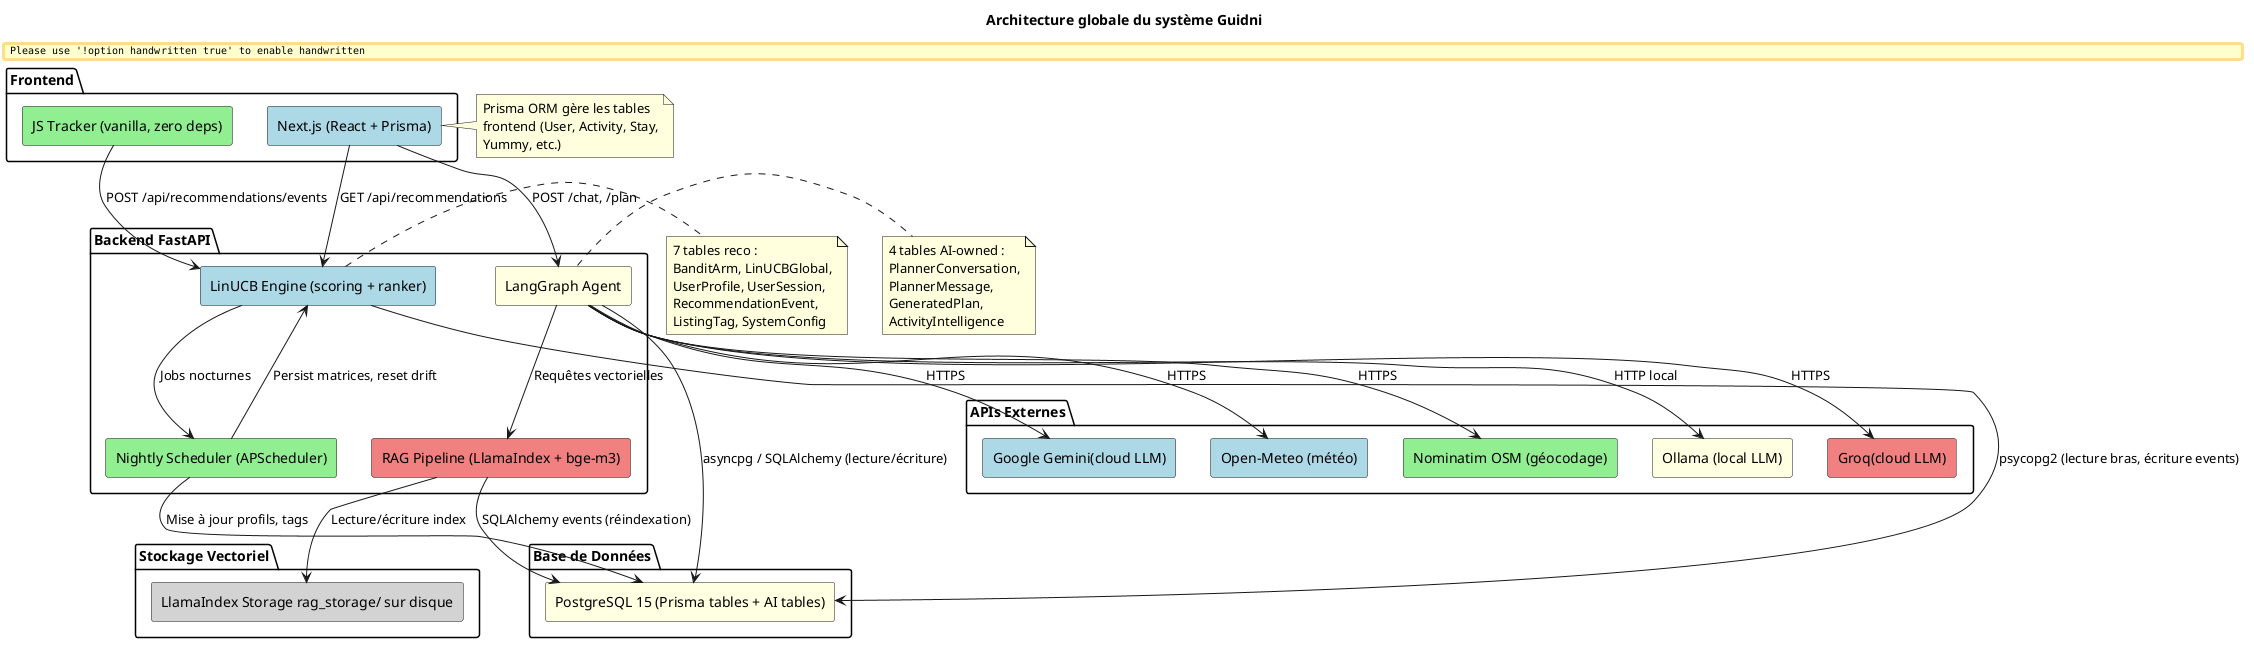
\includegraphics[width=\textwidth]{diagrams/fig_03_global_architecture.png}
    \caption{Les services de la plateforme Guidni}
    \label{fig:services_guidni}
\end{figure}

\subsection{Problématique}

Les systèmes existants échouent à composer les contraintes du voyageur de manière intégrée.
TripAdvisor suggère des attractions individuelles, Booking.com gère l'hébergement isolément,
Google Maps fournit des itinéraires point à point, mais aucune plateforme unifiée n'orchestre
l'ensemble en un plan de voyage cohérent. Le voyageur est contraint de jongler entre plusieurs
applications, un processus fragmenté, chronophage et source de frustrations.

Par ailleurs, le marché touristique de Djerba est fondamentalement trilingue~--- français,
anglais et arabe~--- ce qui impose à tout système de gérer ces trois langues de manière
transparente.

\vspace{0.5cm}
\noindent
\fcolorbox{black}{blue!5}{%
    \parbox{0.95\textwidth}{%
        \vspace{0.3cm}
        \centering
        \textbf{Problématique}\\[0.4cm]
        \begin{minipage}{0.90\textwidth}
        \itshape
        Comment concevoir un système capable de (1)~générer des plans de voyage complets et
        personnalisés via un agent conversationnel multi-outils multilingue, et (2)~recommander
        des contenus touristiques en temps réel grâce à un moteur d'apprentissage en ligne par
        bandits contextuels~?
        \end{minipage}
        \vspace{0.3cm}
    }%
}
\vspace{0.5cm}

\subsection{Objectifs du projet}

Le projet Guidni répond à la problématique à travers quatre objectifs~:


\begin{enumerate}
    \item \textbf{Unification de l'expérience de voyage} : Créer une plateforme intégrée capable d'orchestrer, en une seule interface, la planification complète d'un séjour (hébergement, activités et restorants), éliminant ainsi la fragmentation des outils actuels.
    
    \item \textbf{Assistance autonome} : Développer un agent intelligent capable d'interagir avec le voyageur pour transformer ses besoins complexes en un plan de voyage cohérent et personnalisé.
    
    \item \textbf{Gestion fluide de la diversité linguistique} : Garantir une accessibilité totale au système en assurant un traitement transparent et naturel des interactions en français, anglais et arabe.
    
    \item \textbf{Personnalisation dynamique des recommandations} : Mettre en œuvre un moteur de recommandation capable d'apprendre des préférences de l'utilisateur en temps réel afin d'affiner les suggestions touristiques proposées.
    
    \item \textbf{Évaluation de la fiabilité du système} : Mettre en place un cadre de test robuste pour garantir que le plan généré est non seulement personnalisé, mais également réalisable et pertinent pour le contexte spécifique de Djerba.
\end{enumerate}

\begin{table}[H]
    \centering
    \caption{Tableau des fonctionnalités à concevoir et à implémenter}
    \label{tab:fonctionnalites}
    \small
    \begin{tabular}{c p{5cm} p{6.5cm}}
        \toprule
        \textbf{N°} & \textbf{Fonctionnalité} & \textbf{Description} \\
        \midrule
        F1 & Agent conversationnel multilingue & Chat FR/EN/AR avec mémoire contextuelle \\[3pt]
        F2 & Planification multi-jours & Itinéraires 1--14 jours avec contraintes \\[3pt]
        F3 & Pipeline RAG two-stage & Embeddings bge-m3 + cross-encoder reranker \\[3pt]
        F4 & Moteur LinUCB temps réel & Scoring $<$100\,ms avec cache matriciel \\[3pt]
        F5 & Tracker comportemental & 8 signaux, flush par lot toutes les 15\,s \\[3pt]
        F6 & Réindexation incrémentale & Via événements SQLAlchemy automatiques \\[3pt]
        F7 & Multi-fournisseurs LLM & Ollama, Groq, Gemini, Lightning \\[3pt]
        F8 & Administration système & Rebuild index, health check, configuration \\
        \bottomrule
    \end{tabular}
\end{table}


% ────────────────────────────────────────────────────────────────
\section{Étude de l'existant}
% ────────────────────────────────────────────────────────────────

Avant de proposer une solution, j'ai procédé à une étude comparative des systèmes existants
qui tentent de résoudre des problématiques similaires.

\subsection{Types d'agents LLM}

L'évolution récente des agents LLM permet de distinguer trois générations architecturales~:

\begin{itemize}
    \item \textbf{Agent ReAct simple}~: le LLM alterne librement entre raisonnement et action,
    sans structure d'état. Le risque de boucles infinies et d'hallucinations est élevé.
    \item \textbf{Agent LangGraph (graphe d'états)}~: une machine à états typée contrôle les
    transitions. Chaque nœud encapsule une étape logique (THINK, EXECUTE, VALIDATE, RESPOND).
    \item \textbf{Agent avec pipeline RAG}~: l'agent augmente son raisonnement par la
    récupération de documents pertinents depuis une base de connaissances vectorielle.
\end{itemize}

\begin{figure}[H]
    \centering
    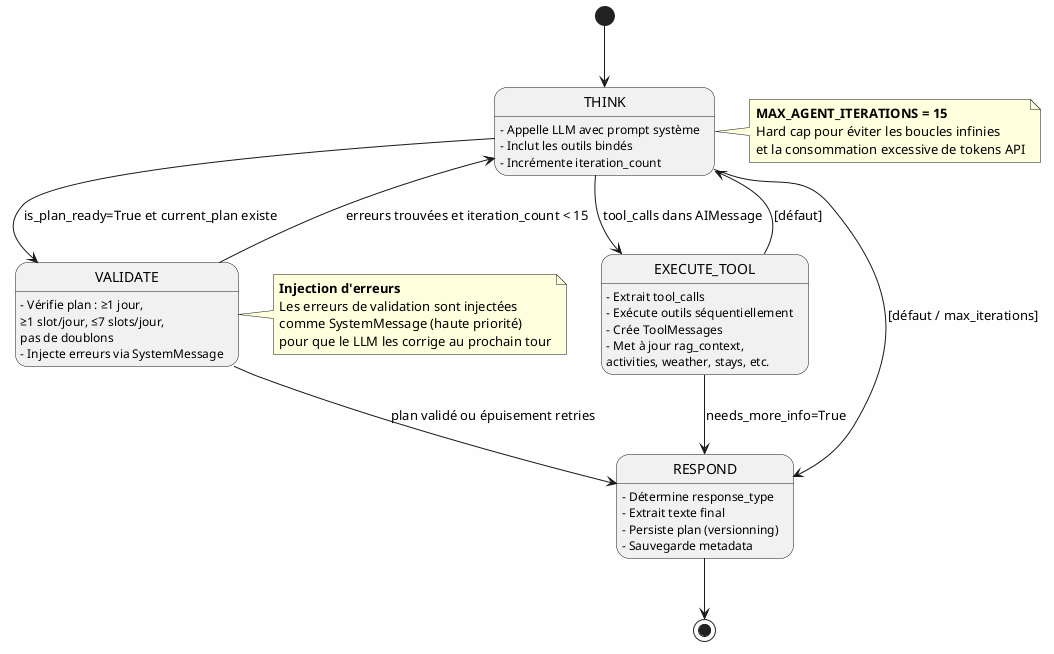
\includegraphics[width=0.65\textwidth]{diagrams/fig_02_langgraph_graph.png}
    \caption{Exemple d'agent LangGraph avec graphe d'états cyclique}
    \label{fig:example_langgraph}
\end{figure}

\begin{figure}[H]
    \centering
    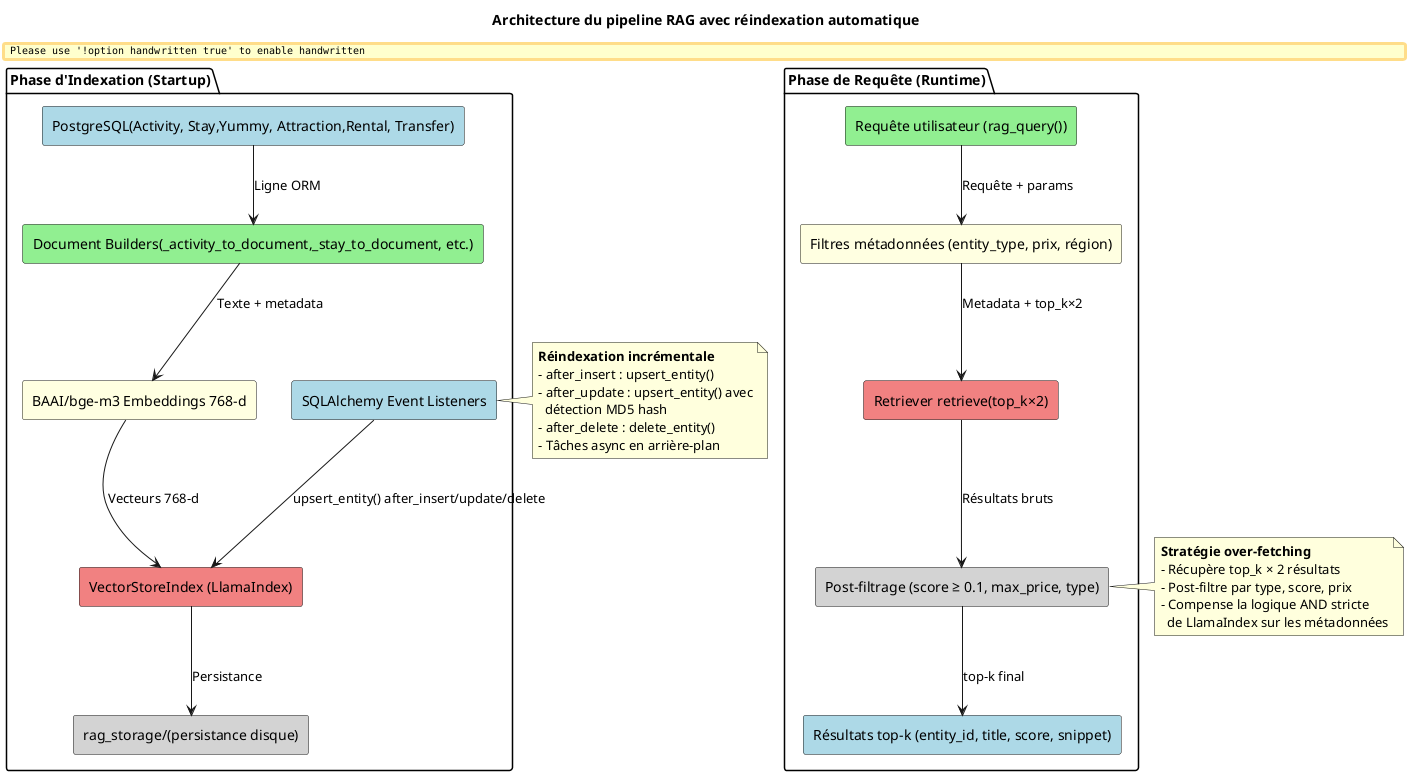
\includegraphics[width=0.85\textwidth]{diagrams/fig_02_rag_architecture.png}
    \caption{Exemple d'agent avec pipeline RAG multilingue}
    \label{fig:example_rag}
\end{figure}

\subsection{Solutions existantes}

\textbf{TripAdvisor} est la plateforme de référence pour les avis touristiques. Elle utilise
un système de recommandation combinant filtrage collaboratif et signaux de contenu, entraîné
hors ligne. Cependant, TripAdvisor recommande des attractions individuelles sans composer
d'itinéraire multi-journées intégré.

\textbf{Booking.com} a développé un système de classement hybride sophistiqué intégrant des
signaux en temps réel~\cite{bernardi2019booking}. Toutefois, ce système est fermé, non
reproductible, et conçu pour un volume de trafic supérieur à celui d'une place de marché locale.

\textbf{ChatGPT / Agents LLM génériques} peuvent formuler des suggestions de voyage, mais
sans accès à des données locales vérifiées, ils produisent des hallucinations factuelles.

\subsection{Critique de l'existant}

Le tableau~\ref{tab:critique_existant} résume les forces et faiblesses des solutions étudiées.

\begin{table}[H]
    \centering
    \caption{Tableau comparatif des solutions existantes}
    \label{tab:critique_existant}
    \small
    \begin{tabular}{p{2.5cm} p{4.5cm} p{4.5cm}}
        \toprule
        \textbf{Solution} & \textbf{Points forts} & \textbf{Points faibles} \\
        \midrule
        TripAdvisor &
        Large base d'avis, couverture mondiale, multilingue &
        Des itinéraires stéréotypés et répétitifs \\[6pt]
        Booking.com &
        Recommandation fiable &
        Système fermé, mono-domaine hébergement \\[6pt]
        ChatGPT &
        Interaction en langage naturel, multilingue &
        Hallucinations, pas de données locales \\[6pt]
        Google Maps &
        Navigation précise, données géographiques fiables &
        Pas de planification multi-jours \\
        \bottomrule
    \end{tabular}
\end{table}

\subsection{Solution proposée~: Guidni}

Face aux lacunes identifiées, je propose \textbf{Guidni}, une plateforme intégrant~:
\begin{itemize}
    \item Un \textbf{Agent Planificateur conversationnel} basé sur LangGraph, doté de 18~outils
    et d'un pipeline RAG multilingue (FR/EN/AR).
    \item Un \textbf{Moteur de Recommandation Hybride LinUCB} exploitant un bandit contextuel
    de dimension~360, apprenant en temps réel.
\end{itemize}

\begin{table}[H]
    \centering
    \caption{Positionnement de Guidni par rapport aux systèmes existants}
    \label{tab:comparaison_guidni}
    \small
    \begin{tabular}{p{2.8cm} c c c c c}
        \toprule
        \textbf{Système} & \textbf{Planif.} & \textbf{Reco. TR} &
        \textbf{Multilingue} & \textbf{Apprent. OL} & \textbf{Open src.} \\
        \midrule
        Guidni & \checkmark & \checkmark & \checkmark & \checkmark & \checkmark \\
        TripAdvisor & $\times$ & $\times$ & \checkmark & $\times$ & $\times$ \\
        Booking.com & $\times$ & \checkmark & \checkmark & \checkmark & $\times$ \\
        ChatGPT & Partiel & $\times$ & \checkmark & $\times$ & $\times$ \\
        \bottomrule
    \end{tabular}
\end{table}


% ────────────────────────────────────────────────────────────────

\section{Choix méthodologique}
% ────────────────────────────────────────────────────────────────

Le choix de la méthodologie de développement constitue une décision structurante pour tout
projet d'ingénierie logicielle. J'ai étudié trois méthodologies candidates avant de retenir
celle la plus adaptée au projet Guidni.

\subsection{Étude comparative des méthodologies}

\begin{table}[H]
    \centering
    \caption{Tableau comparatif des méthodologies de développement}
    \label{tab:methodo_comparaison}
    \small
    \begin{tabular}{p{2.2cm} p{3.8cm} p{3.8cm} p{3.8cm}}
        \toprule
        \textbf{Critère} & \textbf{Scrum} & \textbf{2TUP} & \textbf{Kanban} \\
        \midrule
        \textbf{Description} &
        Cadre Agile itératif par Sprints de 2--4 semaines &
        Processus à deux branches (fonctionnelle / technique) &
        Flux continu sans itérations fixes \\[6pt]
        \textbf{Points forts} &
        Adaptation rapide, Sprint Reviews, livrables incrémentaux &
        Séparation fonctionnel/technique, rigueur &
        Flexibilité maximale, visualisation du flux \\[6pt]
        \textbf{Points faibles} &
        Cérémonies parfois lourdes &
        Rigidité face aux changements &
        Absence de rythme structuré \\
        \bottomrule
    \end{tabular}
\end{table}

\subsection{Méthodologie retenue~: Scrum}

J'ai retenu la méthodologie \textbf{Scrum} pour les raisons suivantes~:
\begin{itemize}
    \item La complexité de l'hybridation agent LLM / algorithme LinUCB impose une approche
    itérative permettant de valider chaque composant incrémentalement.
    \item Les livrables fonctionnels par Sprint offrent une visibilité constante validée par
    les Sprint Reviews avec l'encadrant.
    \item La \textbf{Definition of Done} (DoD) garantit un critère de qualité objectif.
\end{itemize}


\begin{figure}[H]
    \centering
    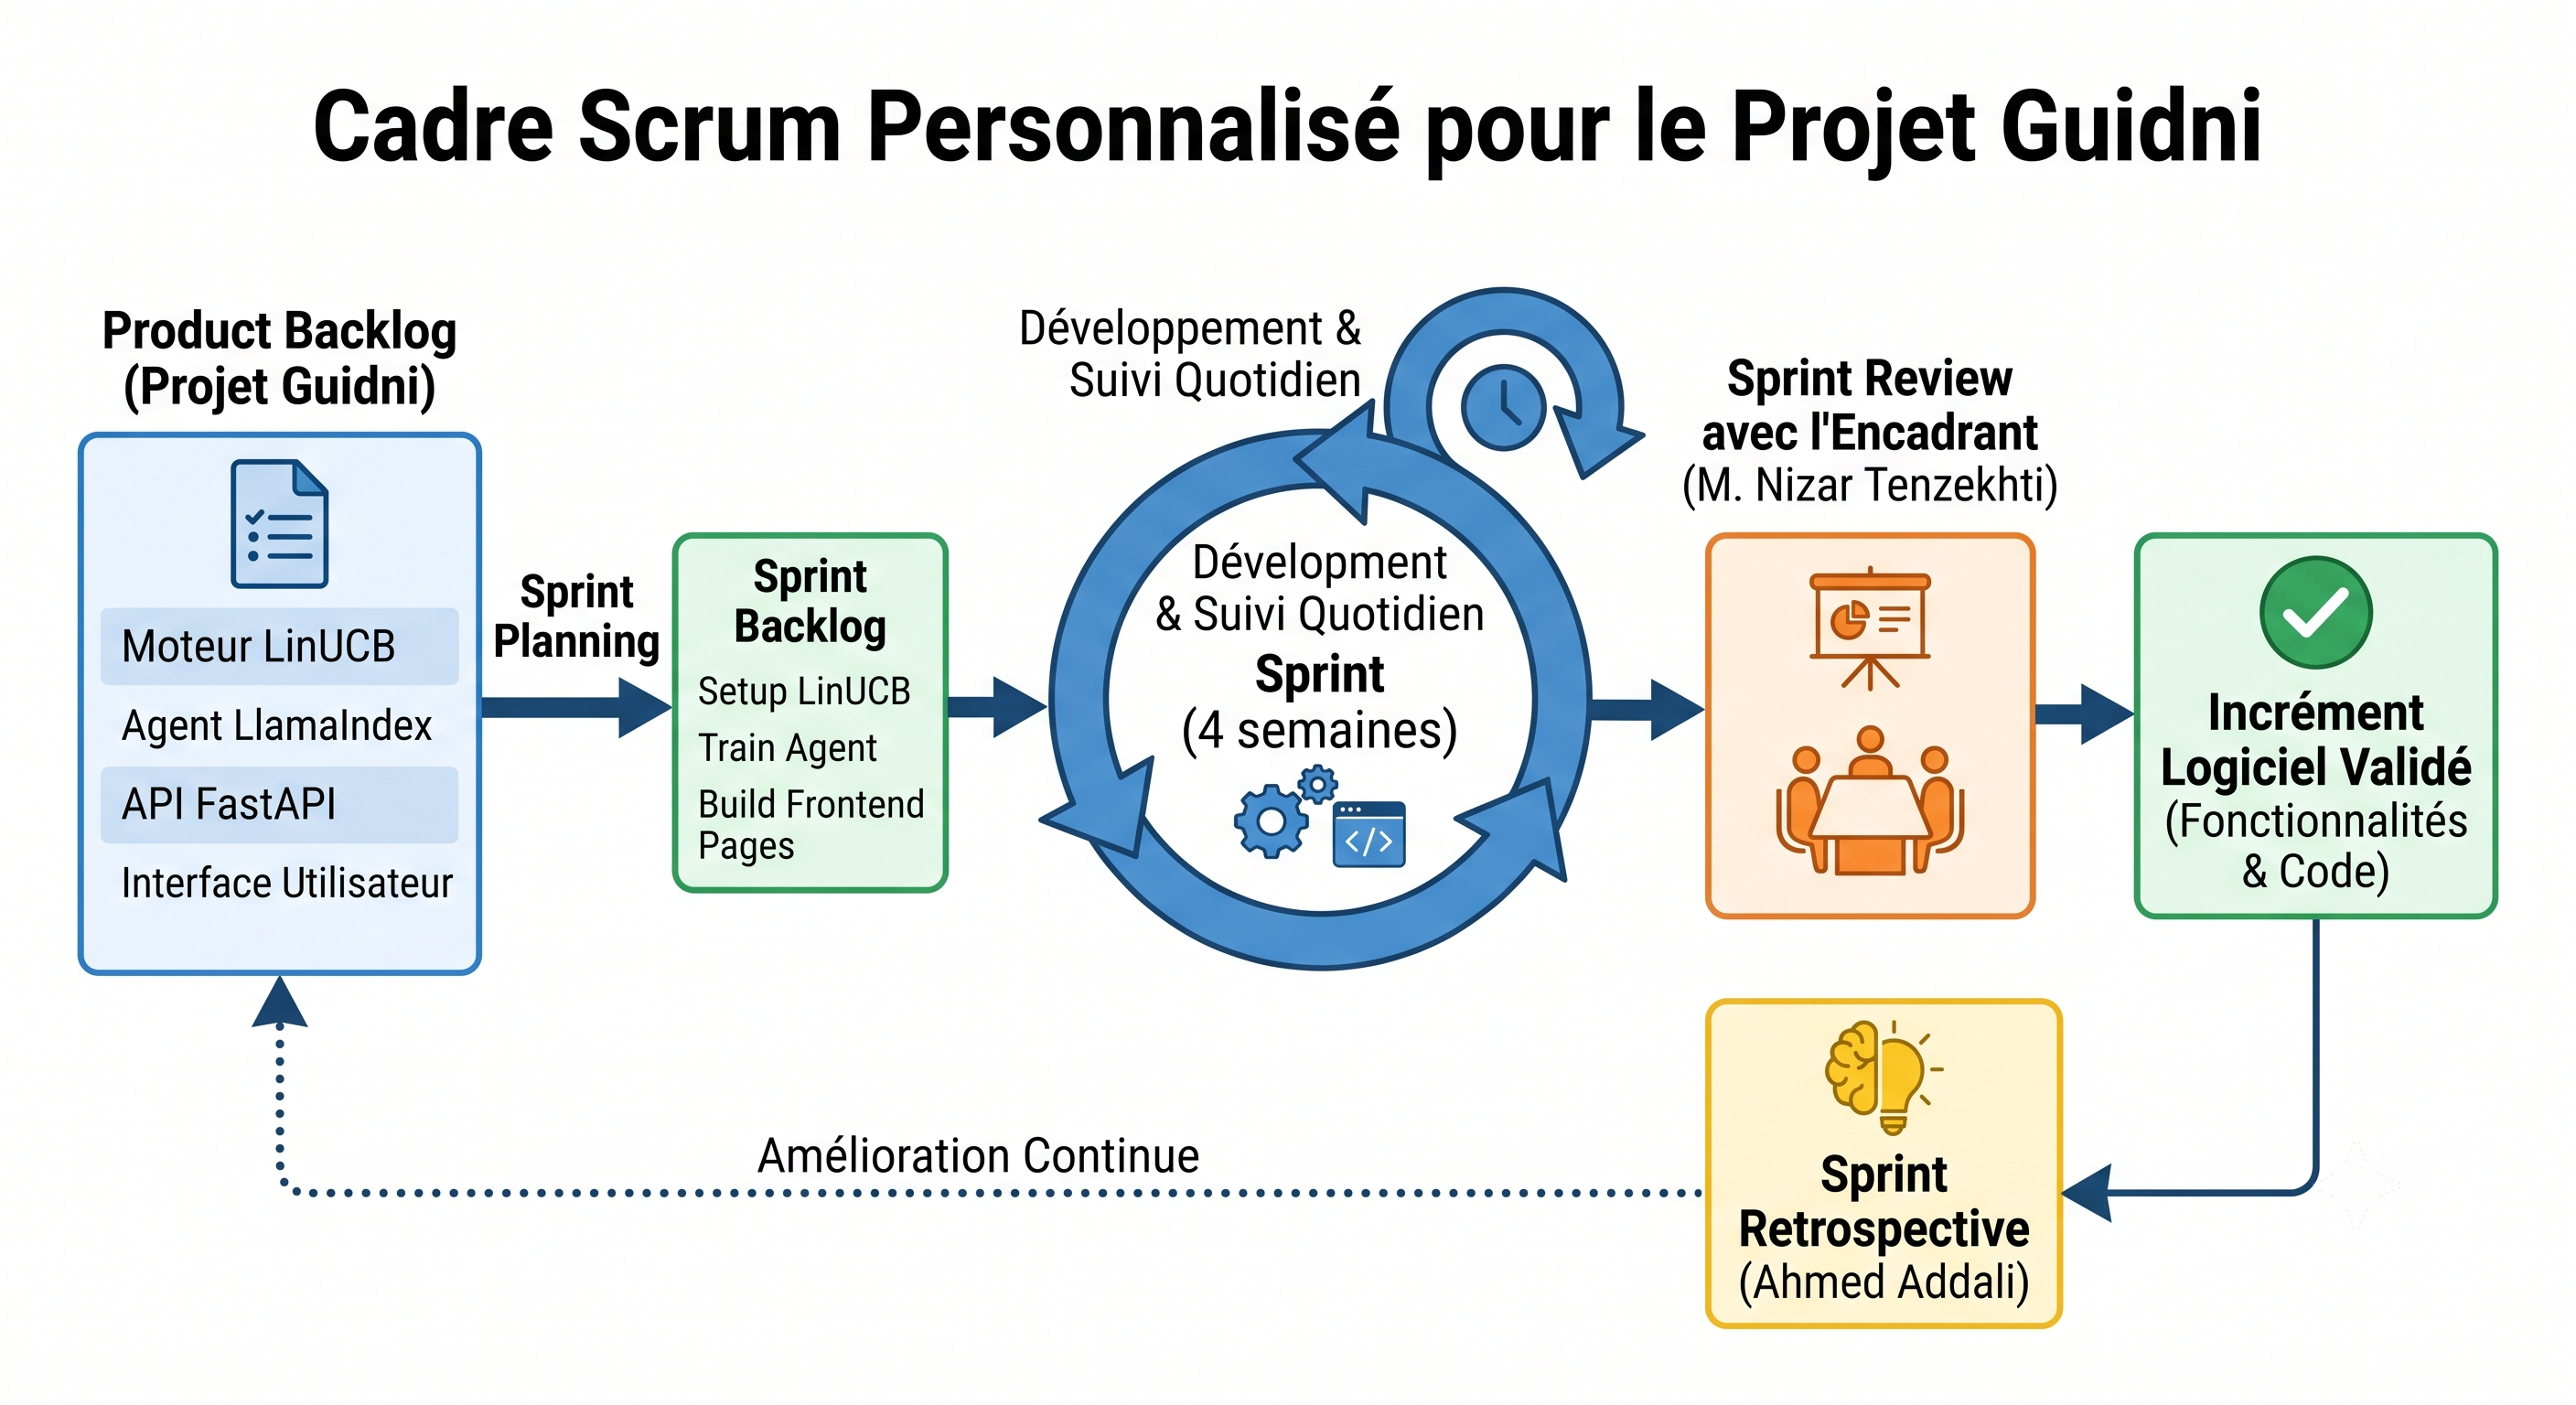
\includegraphics[width=0.85\textwidth]{images/fig_01_scrum_process.png}
    \caption{Processus Scrum appliqué au projet Guidni}
    \label{fig:scrum_process}
\end{figure}


% ────────────────────────────────────────────────────────────────
\section*{Conclusion}
\addcontentsline{toc}{section}{Conclusion}

Ce premier chapitre a permis de présenter le cadre général du projet Guidni. J'ai introduit
l'organisme d'accueil, décrit le contexte et la problématique liée à l'absence d'outils de
planification touristique intelligents pour Djerba. L'étude de l'existant a mis en évidence
les lacunes des solutions actuelles, ce qui a motivé la proposition de Guidni. Enfin, le choix
de Scrum a été justifié par sa capacité à gérer la complexité itérative du projet.

Le chapitre suivant sera consacré au lancement du projet, incluant l'analyse des besoins, les
définitions théoriques, le Product Backlog et la planification des Sprints.


\chapter{Lancement du Projet}
% ============================================================================
% CHAPITRE 2 — LANCEMENT DU PROJET
% ============================================================================

\section{Introduction}

Ce chapitre est consacré au lancement du projet Guidni. Il vise à poser les bases nécessaires
avant d'entamer le développement itératif par Sprints. Pour cela, j'ai suivi le plan suivant~:
\begin{enumerate}
    \item Analyse et spécification des besoins fonctionnels et non fonctionnels
    \item Définitions théoriques des concepts clés
    \item Architecture fonctionnelle et logique
    \item Product Backlog
    \item Planification des Sprints
    \item Environnement de travail et outils
\end{enumerate}


% ────────────────────────────────────────────────────────────────
\section{Analyse des besoins}
% ────────────────────────────────────────────────────────────────

\subsection{Identification des acteurs}

Le système Guidni fait intervenir trois acteurs principaux~:

\begin{itemize}
    \item Le \textbf{Touriste}~: acteur principal qui interagit avec l'interface de chat pour
    formuler des demandes de planification, recevoir des itinéraires, et consulter des
    recommandations. Son comportement de navigation est automatiquement capté par le tracker
    JavaScript pour alimenter le moteur de recommandation.

    \item L'\textbf{Administrateur}~: responsable de la supervision technique. Il peut
    déclencher une reconstruction de l'index RAG, consulter l'état de santé du système et
    configurer le fournisseur LLM par défaut.

    \item Le \textbf{Système}~: ensemble des processus automatisés (écouteurs SQLAlchemy,
    tracker JavaScript, jobs nocturnes APScheduler, persistance des matrices LinUCB).
\end{itemize}

\subsection{Besoins fonctionnels}

Les besoins fonctionnels du système sont les suivants~:
\begin{itemize}
    \item \textbf{BF-01}~: Formuler des requêtes en langage naturel multilingue (FR/EN/AR)
    \item \textbf{BF-02}~: Générer des itinéraires multi-jours personnalisés (1 à 14~jours)
    \item \textbf{BF-03}~: Modifier un plan existant par des messages de suivi conversationnels
    \item \textbf{BF-04}~: Effectuer des recherches sémantiques dans le catalogue touristique
    \item \textbf{BF-05}~: Intégrer les données météorologiques en temps réel (Open-Meteo)
    \item \textbf{BF-06}~: Calculer les distances entre les sites (Haversine / Nominatim)
    \item \textbf{BF-07}~: Afficher des recommandations personnalisées en temps réel
    \item \textbf{BF-08}~: Collecter les signaux comportementaux du touriste
    \item \textbf{BF-09}~: Apprendre en ligne à partir des récompenses utilisateur
    \item \textbf{BF-10}~: Consulter et archiver l'historique des conversations
\end{itemize}

\subsection{Besoins non fonctionnels}

\begin{table}[H]
    \centering
    \caption{Besoins non fonctionnels du système Guidni}
    \label{tab:bnf}
    \small
    \begin{tabular}{p{2.8cm} p{5cm} p{5cm}}
        \toprule
        \textbf{Catégorie} & \textbf{Besoin} & \textbf{Cible} \\
        \midrule
        Performance & Latence endpoint \texttt{/chat} & $< 5$\,s (P95) \\
         & Latence recommandation & $< 100$\,ms (P95) \\[3pt]
        Disponibilité & Uptime du service & 99,5\% \\[3pt]
        Sécurité & Validation utilisateur & Vérification \texttt{user\_id} par requête \\
         & Limitation de débit & 10 événements/annonce/session \\[3pt]
        Multilingue & Langues supportées & FR, EN, AR (auto-détection) \\[3pt]
        Confidentialité & Données vers LLM & Pas de PII sans consentement \\
         & Option locale & Ollama pour souveraineté complète \\
        \bottomrule
    \end{tabular}
\end{table}

\subsection{Diagramme des cas d'utilisation global}

Le diagramme suivant présente une vue d'ensemble des interactions entre les trois acteurs
et les fonctionnalités principales du système.

\begin{figure}[H]
    \centering
    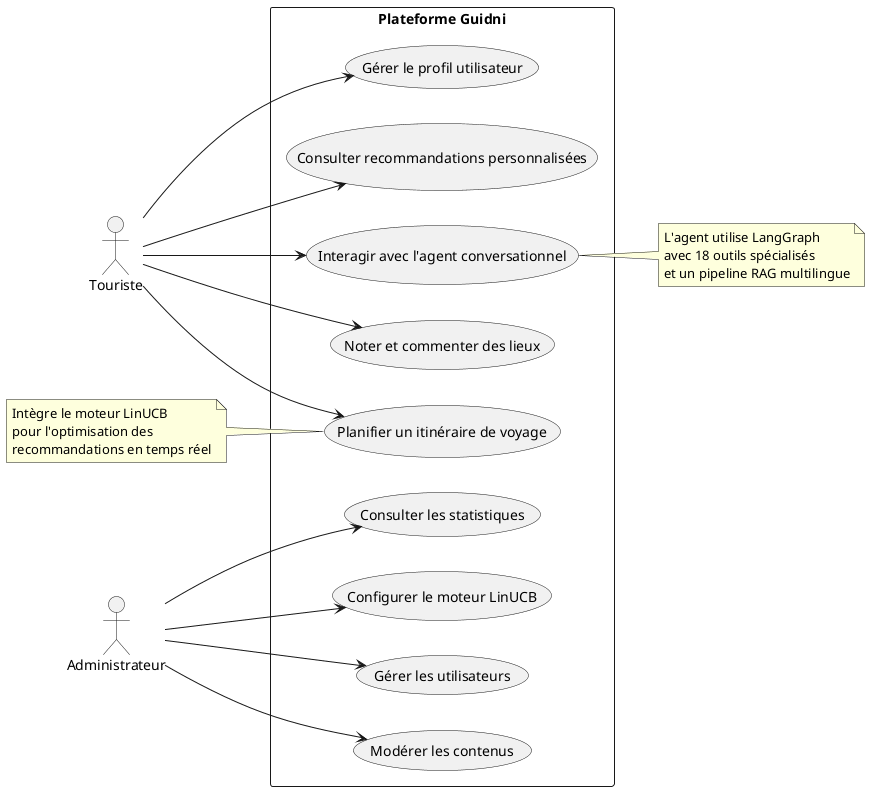
\includegraphics[width=\textwidth]{diagrams/plantuml/usecase_global.png}
    \caption{Diagramme de cas d'utilisation global du système Guidni}
    \label{fig:use_case_global}
\end{figure}


% ────────────────────────────────────────────────────────────────
\section{Définitions théoriques}
% ────────────────────────────────────────────────────────────────

Cette section présente les concepts théoriques fondamentaux sur lesquels repose le système
Guidni. Chaque concept est défini puis illustré par son application concrète dans le projet.

\subsection{Grands modèles de langage (LLM)}

L'architecture Transformer, introduite par Vaswani et al.~\cite{vaswani2017attention},
constitue le socle de tous les LLMs modernes. Son mécanisme d'attention multi-têtes permet de
pondérer l'importance relative de chaque token. L'ajustement par instructions et le RLHF
transforment un modèle de prédiction de tokens en un assistant capable d'exécuter des
instructions en langage naturel. L'appel d'outils (\textit{function calling}) permet au LLM
d'émettre un objet JSON structuré décrivant une fonction externe à appeler, plutôt que de
générer la réponse depuis sa mémoire paramétrique.

\begin{figure}[H]
    \centering
    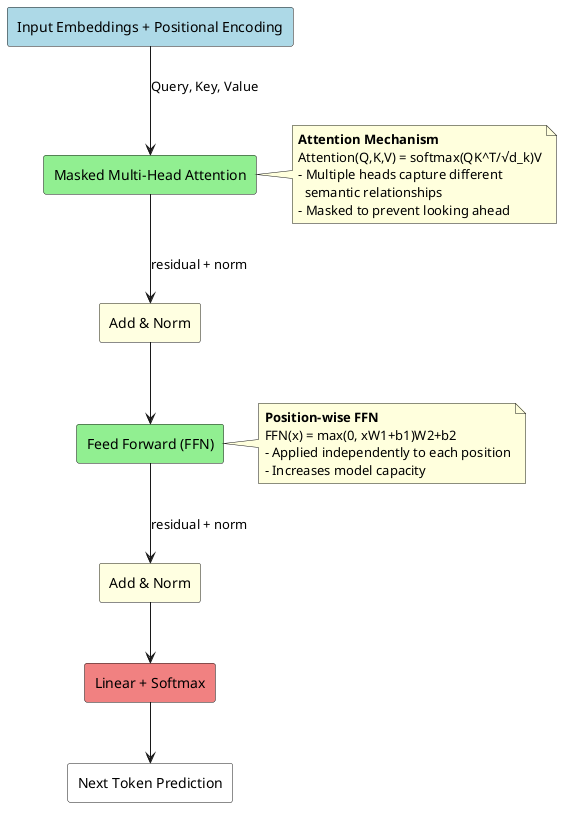
\includegraphics[width=0.75\textwidth]{diagrams/fig_02_transformer_attention.png}
    \caption{Architecture du Transformer avec mécanisme d'attention multi-têtes}
    \label{fig:transformer_arch}
\end{figure}

\subsection{Framework agentique LangGraph}

LangGraph, développé par LangChain Inc., étend le patron ReAct (\textit{Reason + Act})
proposé par Yao et al.~\cite{yao2023react} avec une machine à états typée explicite.
L'état de l'agent est défini par un \texttt{TypedDict} Python (\texttt{AgentState}) qui
accumule les messages, profils, données géolocalisées, compteurs de sécurité et indicateurs
décisionnels. Des fonctions de routage conditionnel déterminent quel nœud s'exécute ensuite.

Le graphe Guidni comporte quatre nœuds~: \textbf{THINK} (raisonnement du LLM),
\textbf{EXECUTE\_TOOL} (exécution d'un outil), \textbf{VALIDATE} (vérification du plan)
et \textbf{RESPOND} (formulation de la réponse). Une sortie forcée à 15~itérations empêche
les boucles infinies.

\begin{figure}[H]
    \centering
    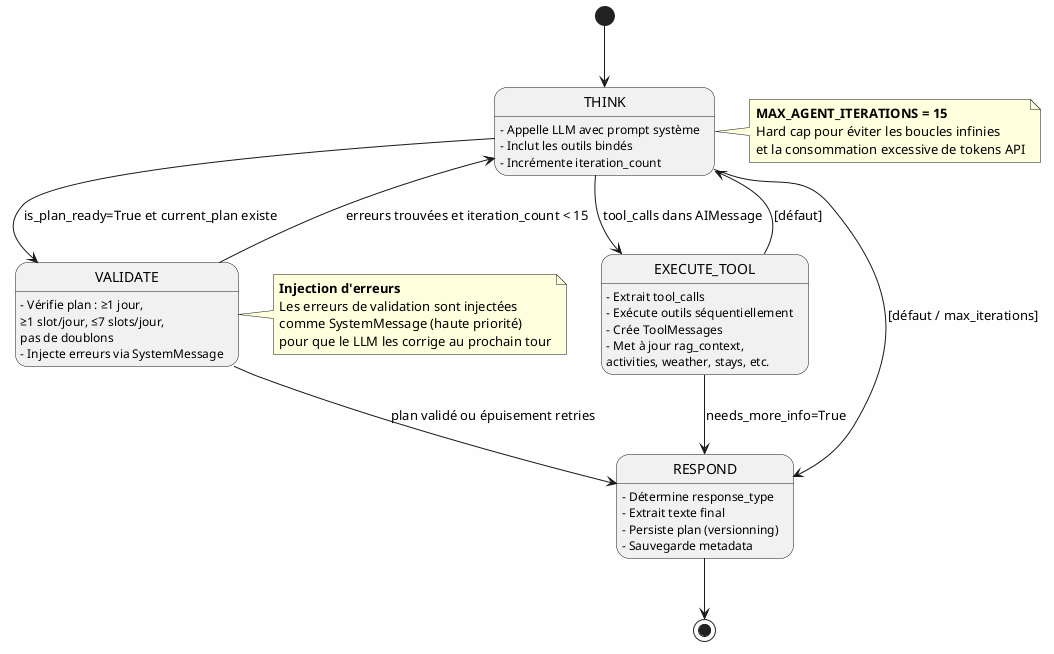
\includegraphics[width=0.7\textwidth]{diagrams/fig_02_langgraph_graph.png}
    \caption{Architecture LangGraph --- graphe d'états cyclique de l'agent}
    \label{fig:langgraph_arch}
\end{figure}

\subsection{Génération augmentée par récupération (RAG)}

Le principe RAG, formalisé par Lewis et al.~\cite{lewis2020rag}, consiste à récupérer des
documents pertinents depuis une base de connaissances et les injecter dans le prompt du LLM.
Le pipeline Guidni utilise BAAI/bge-m3 (embeddings multilingues 1024~dimensions, 100+~langues)
en première étape de récupération, suivi de bge-reranker-v2-m3 (cross-encoder) pour le
réordonnancement. L'index est maintenu à jour par réindexation incrémentale via les événements
SQLAlchemy (\texttt{after\_insert}, \texttt{after\_update}, \texttt{after\_delete}).

\begin{figure}[H]
    \centering
    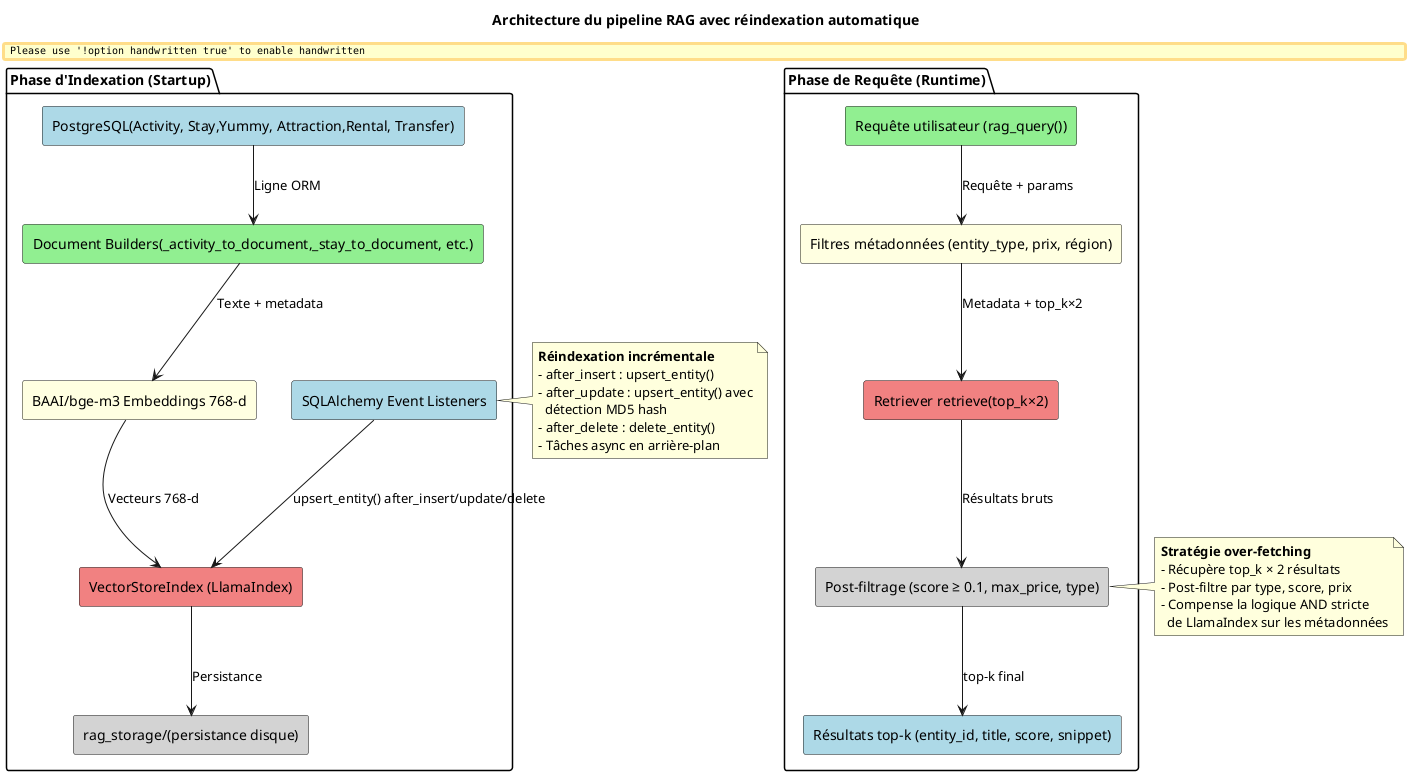
\includegraphics[width=0.85\textwidth]{diagrams/fig_02_rag_architecture.png}
    \caption{Architecture du pipeline RAG multilingue}
    \label{fig:rag_arch}
\end{figure}

\subsection{Bandits contextuels et algorithme LinUCB}

L'algorithme LinUCB~\cite{li2010linucb} suppose que la récompense espérée est une fonction
linéaire du vecteur de contexte~: $\mathbb{E}[r|\phi] = \theta^\top \phi$. Le score UCB
combine exploitation et exploration~:
\begin{equation}
    \text{score} = \underbrace{\hat{\theta}^\top \phi}_{\text{exploitation}} +
    \underbrace{\alpha \sqrt{\phi^\top A^{-1} \phi}}_{\text{exploration}}
    \label{eq:ucb_score}
\end{equation}

Le vecteur $\phi$ de dimension~306 est construit par produit de Kronecker~:
$\phi = x_{\text{user}}(9) \otimes x_{\text{tags}}(34)$, combinant le contexte utilisateur
(heure, mois, défilement, budget, type de voyage) avec les tags binaires des annonces.

\begin{figure}[H]
    \centering
    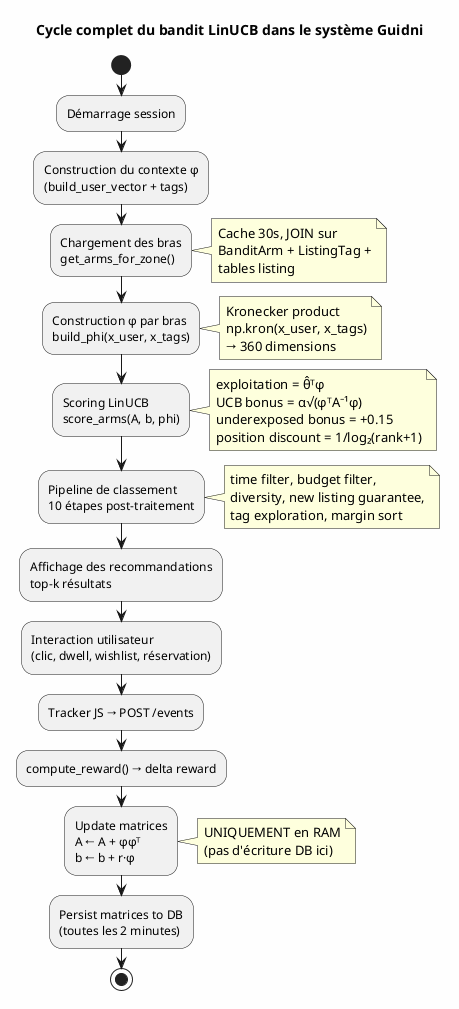
\includegraphics[width=0.7\textwidth]{diagrams/fig_02_linucb_cycle.png}
    \caption{Cycle exploitation / exploration du LinUCB}
    \label{fig:linucb_cycle}
\end{figure}

\begin{table}[H]
    \centering
    \caption{Étude comparative des approches de recommandation}
    \label{tab:reco_approaches}
    \small
    \begin{tabular}{p{3cm} p{2cm} p{2cm} p{2.5cm} p{2cm}}
        \toprule
        \textbf{Approche} & \textbf{Cold Start} & \textbf{Dérive} &
        \textbf{Données} & \textbf{Guidni~?} \\
        \midrule
        Filtrage collaboratif & Problématique & Mauvaise & Grand historique & Non \\[3pt]
        Basé contenu & Acceptable & Mauvaise & Attributs items & Partiel \\[3pt]
        Hybride offline & Partiel & Mauvaise & Les deux & Non \\[3pt]
        LinUCB contextuel & Bonus exploration & Reset $\lambda$-decay & Contexte TR & \textbf{Oui} \\
        \bottomrule
    \end{tabular}
\end{table}


% ────────────────────────────────────────────────────────────────
\section{Architecture fonctionnelle et logique}
% ────────────────────────────────────────────────────────────────

\subsection{Architecture fonctionnelle}

Le système Guidni repose sur l'articulation de deux sous-systèmes partageant une base de
données PostgreSQL 15 unifiée~:

\begin{itemize}
    \item Le \textbf{frontend} Next.js / Prisma gère l'interface utilisateur et les opérations
    CRUD sur les entités touristiques.
    \item Le \textbf{backend IA} FastAPI héberge l'agent planificateur LangGraph
    (9~endpoints REST) et le moteur de recommandation LinUCB (3~endpoints REST).
\end{itemize}

\begin{figure}[H]
    \centering
    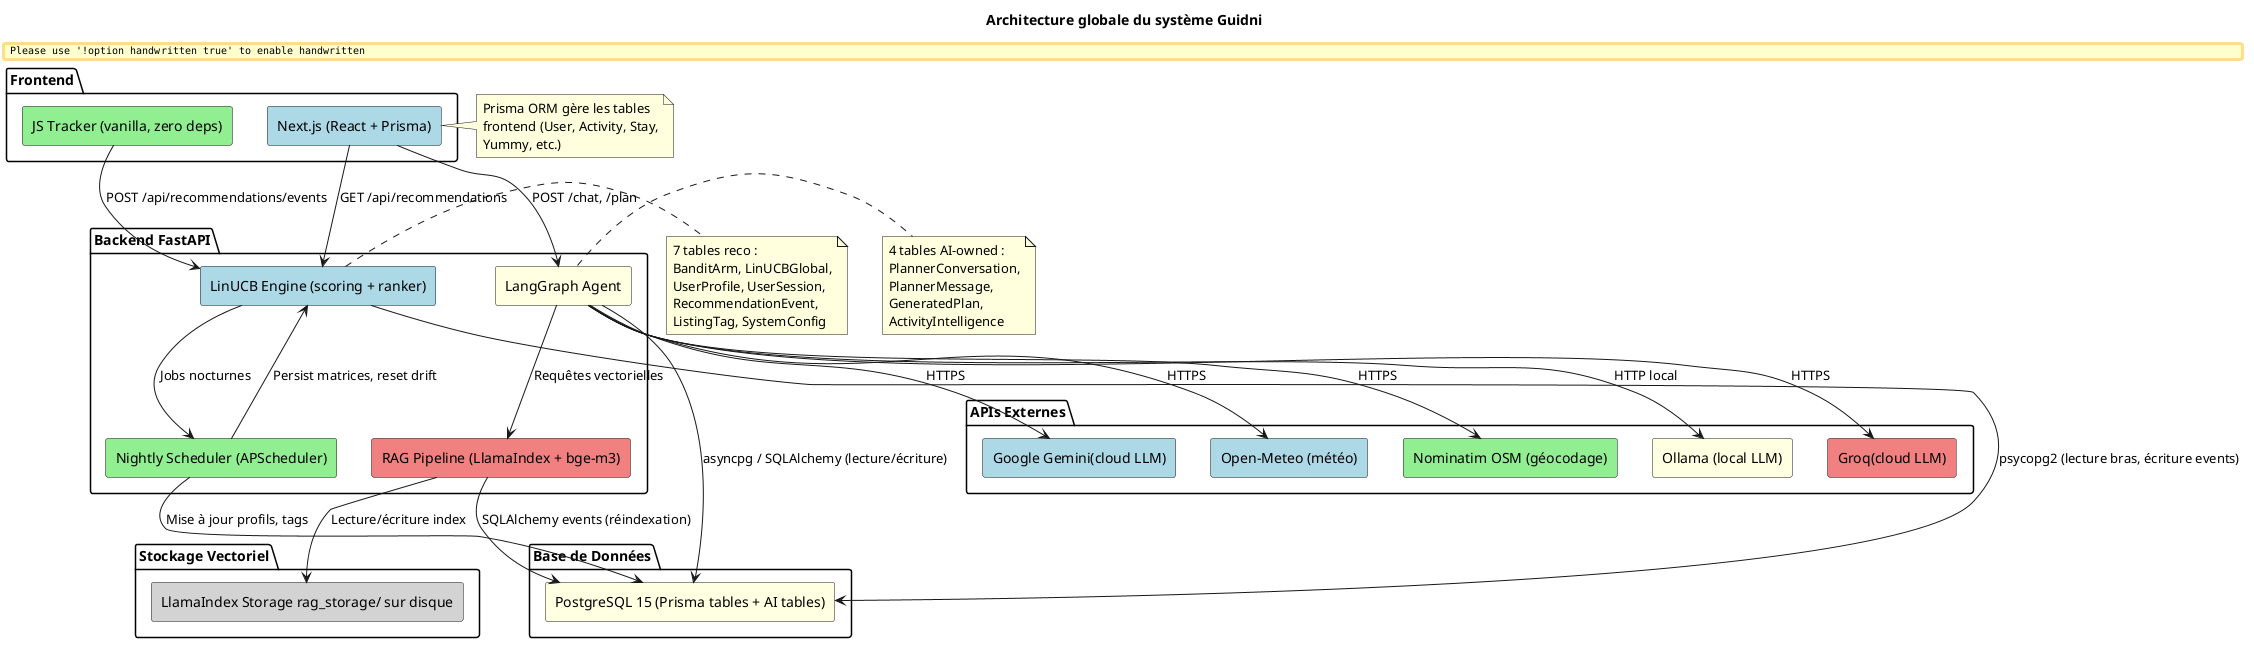
\includegraphics[width=\textwidth]{diagrams/fig_03_global_architecture.png}
    \caption{Architecture fonctionnelle du système Guidni}
    \label{fig:global_arch}
\end{figure}

\subsection{Architecture logique en couches}

L'architecture est organisée en quatre couches~:
\begin{enumerate}
    \item \textbf{Couche de présentation}~: endpoints FastAPI, schémas Pydantic, middleware CORS
    \item \textbf{Couche de logique métier}~: agent LangGraph (4~nœuds, 18~outils), moteur
    LinUCB (pipeline 10~étapes), moteur de requête RAG
    \item \textbf{Couche d'accès aux données}~: modèles SQLAlchemy, index LlamaIndex, pool
    psycopg2
    \item \textbf{Couche d'infrastructure}~: moteur AsyncPG, APScheduler, journalisation
    rotative
\end{enumerate}

\begin{figure}[H]
    \centering
    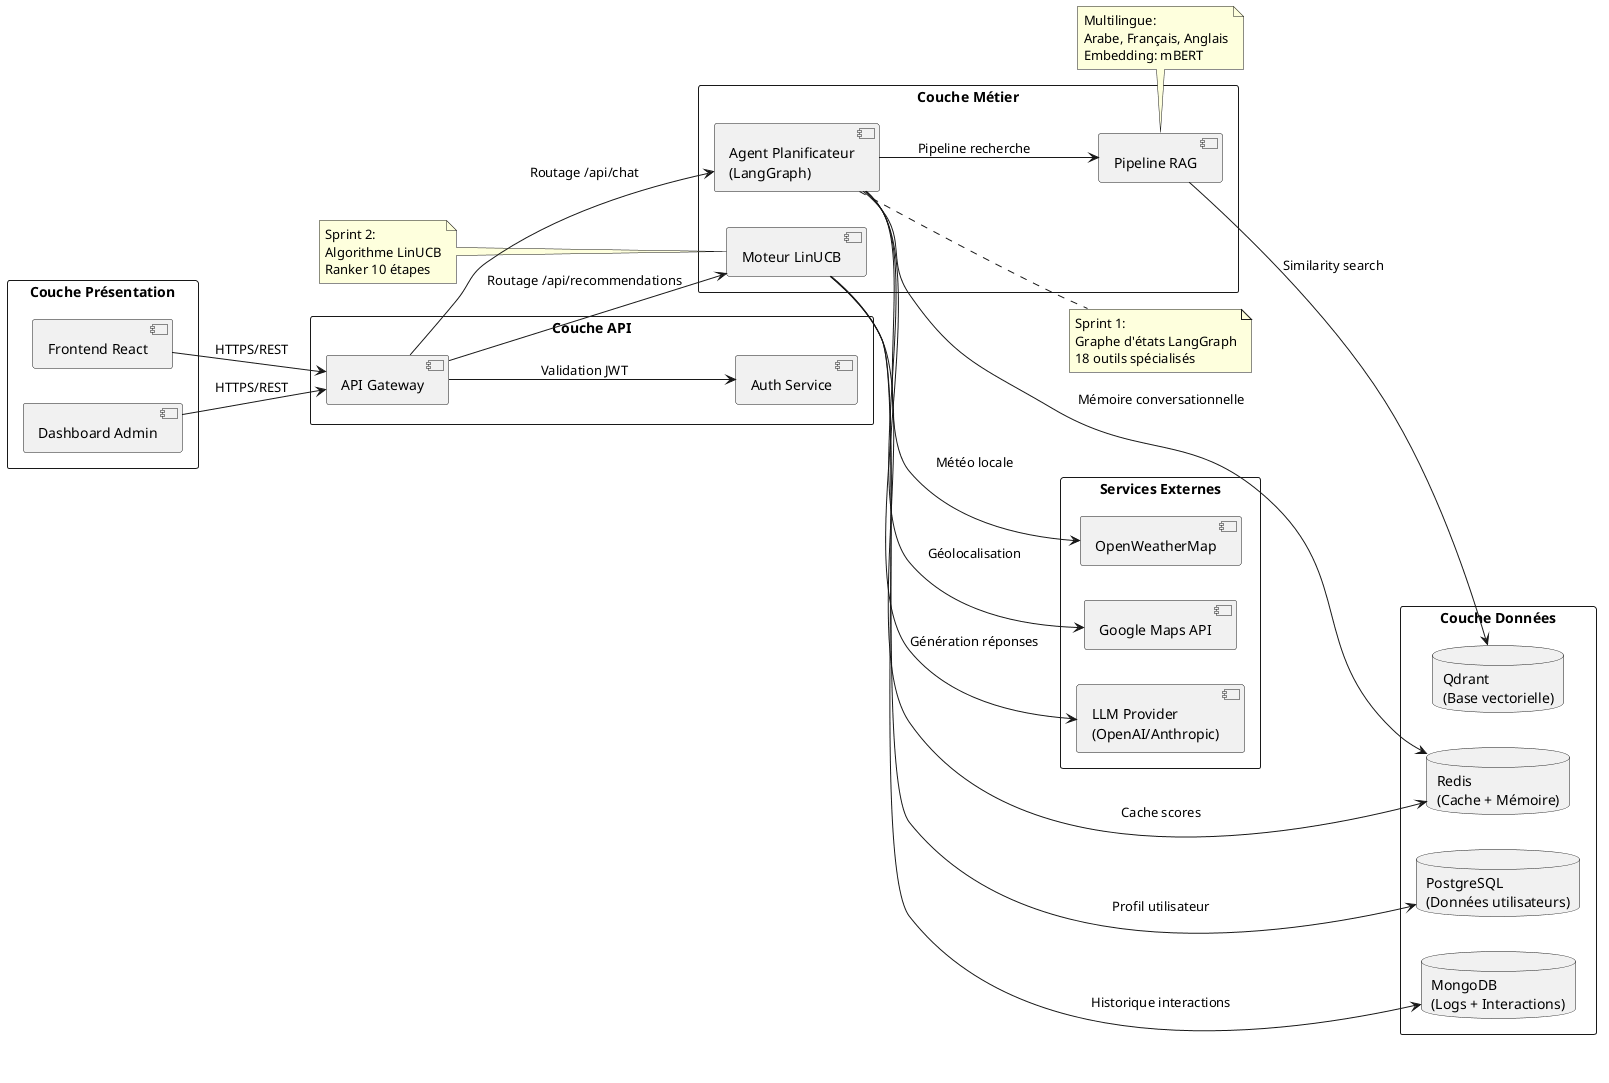
\includegraphics[width=\textwidth]{diagrams/plantuml/class_architecture.png}
    \caption{Architecture logique en couches du système Guidni}
    \label{fig:arch_logique}
\end{figure}

\subsection{Diagramme de cas d'utilisation global détaillé}

\begin{figure}[H]
    \centering
    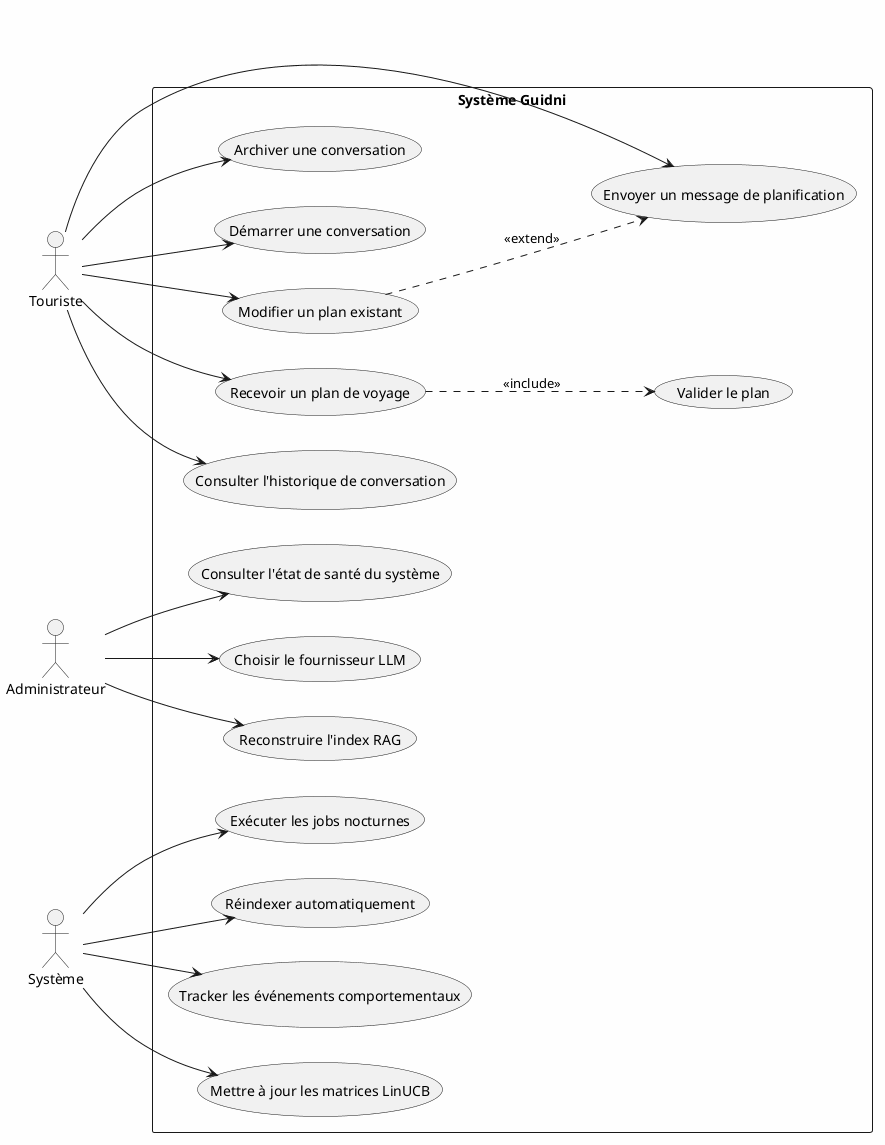
\includegraphics[width=\textwidth]{diagrams/fig_03_use_case_global.png}
    \caption{Diagramme de cas d'utilisation global détaillé}
    \label{fig:uc_global_detail}
\end{figure}

\subsection{Conception de la base de données}

Le backend IA lit 14~tables Prisma en lecture seule et possède en écriture 4~tables
planificateur et 7~tables recommandation.

\begin{figure}[H]
    \centering
    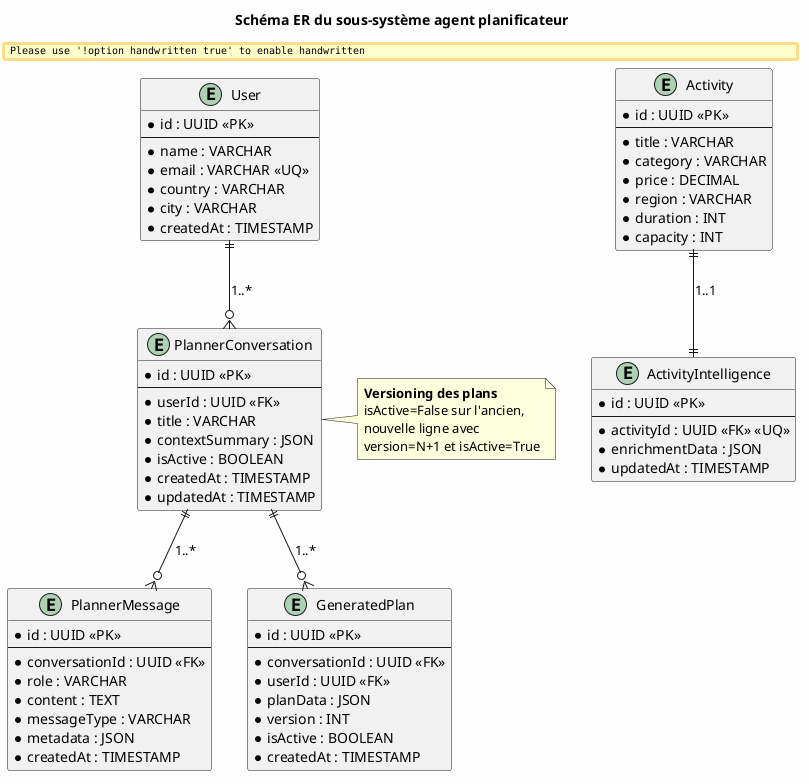
\includegraphics[width=\textwidth]{diagrams/fig_03_er_diagram_planner.png}
    \caption{Schéma ER du sous-système agent planificateur}
    \label{fig:er_planner}
\end{figure}

\begin{figure}[H]
    \centering
    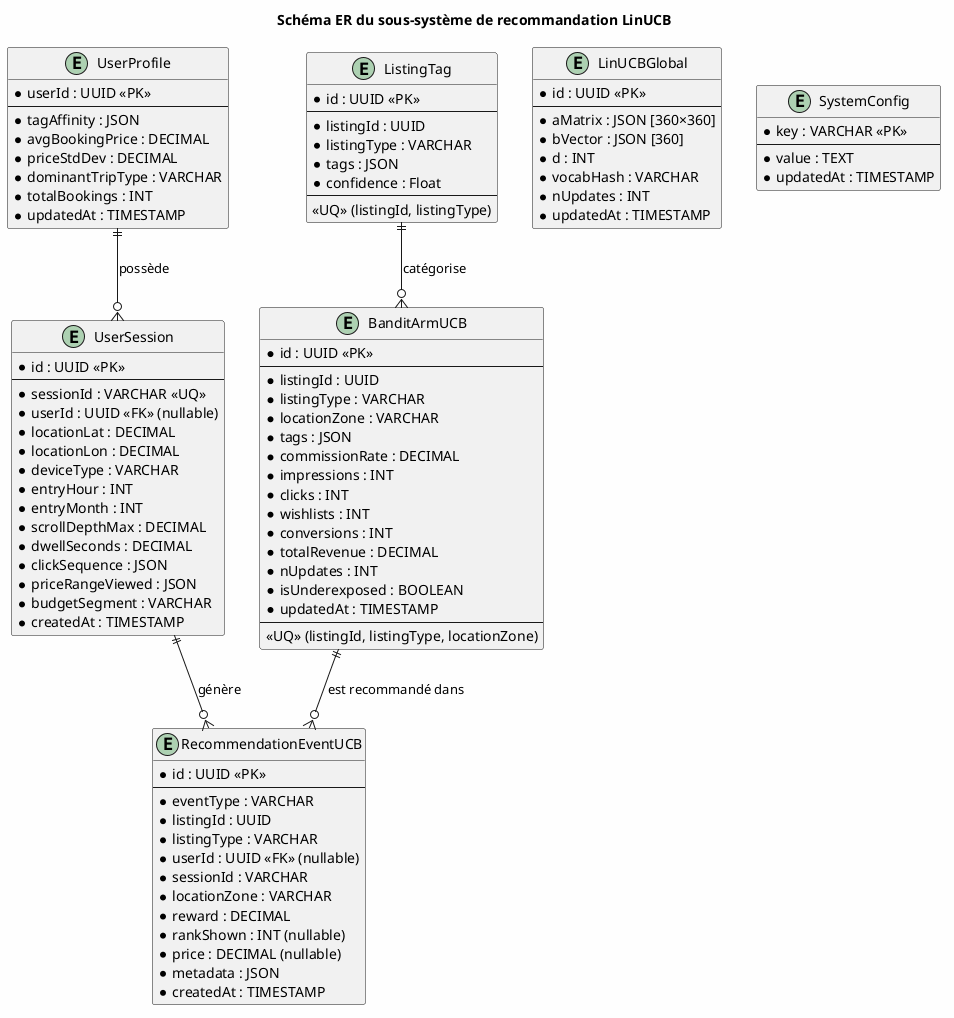
\includegraphics[width=\textwidth]{diagrams/fig_03_er_diagram_recommender.png}
    \caption{Schéma ER du sous-système de recommandation LinUCB}
    \label{fig:er_recommender}
\end{figure}


% ────────────────────────────────────────────────────────────────
\section{Product Backlog}
% ────────────────────────────────────────────────────────────────

Le Product Backlog recense l'ensemble des User Stories du projet, priorisées selon la méthode
MoSCoW (\textit{Must / Should / Could / Won't}).

\begin{table}[H]
    \centering
    \caption{Product Backlog du projet Guidni}
    \label{tab:product_backlog}
    \small
    \begin{tabular}{c p{9cm} c}
        \toprule
        \textbf{ID} & \textbf{User Story} & \textbf{Priorité} \\
        \midrule
        US-01 & En tant que touriste, je veux formuler des requêtes en langage naturel
        multilingue (FR/EN/AR) & Must \\[3pt]
        US-02 & En tant que touriste, je veux recevoir un itinéraire multi-jours personnalisé
        selon mon budget et mes préférences & Must \\[3pt]
        US-03 & En tant que touriste, je veux modifier mon plan par des messages de suivi & Must \\[3pt]
        US-04 & En tant que système, je veux effectuer des recherches sémantiques RAG dans le
        catalogue touristique & Must \\[3pt]
        US-05 & En tant que système, je veux intégrer les données météo en temps réel & Should \\[3pt]
        US-06 & En tant que système, je veux scorer les recommandations en $<$100\,ms grâce
        au cache matriciel LinUCB & Must \\[3pt]
        US-07 & En tant que touriste, je veux recevoir des recommandations adaptées à mon
        comportement de navigation & Must \\[3pt]
        US-08 & En tant que système, je veux collecter les signaux comportementaux du touriste
        via un tracker JavaScript & Must \\[3pt]
        US-09 & En tant qu'administrateur, je veux reconstruire l'index RAG & Should \\[3pt]
        US-10 & En tant que touriste, je veux consulter l'historique de mes conversations & Could \\[3pt]
        US-11 & En tant que système, je veux maintenir les profils utilisateurs via des jobs
        nocturnes & Should \\[3pt]
        US-12 & En tant que système, je veux vérifier l'intégrité du vocabulaire de tags par
        hachage SHA-256 & Must \\
        \bottomrule
    \end{tabular}
\end{table}


% ────────────────────────────────────────────────────────────────
\section{Planification des Sprints}
% ────────────────────────────────────────────────────────────────

Le tableau~\ref{tab:sprint_planning} présente la planification globale des quatre Sprints
du projet.

\begin{table}[H]
    \centering
    \caption{Planification des Sprints du projet Guidni}
    \label{tab:sprint_planning}
    \small
    \begin{tabular}{c c p{6.5cm} c}
        \toprule
        \textbf{Release} & \textbf{Sprint} & \textbf{Objectif} & \textbf{Période} \\
        \midrule
        \multirow{2}{*}{R1} & Sprint 1 & Mise en place de l'environnement, interface
        utilisateur et architecture de base & Oct. 2024 \\[3pt]
         & Sprint 2 & Implémentation du pipeline RAG multilingue et recherche sémantique &
        Nov. 2024 \\[3pt]
        \multirow{2}{*}{R2} & Sprint 3 & Agent LLM, machine à états LangGraph et planification
        conversationnelle & Déc. 2024 \\[3pt]
         & Sprint 4 & Moteur de recommandation LinUCB, tests et évaluation &
        Jan.--Fév. 2025 \\
        \bottomrule
    \end{tabular}
\end{table}

\begin{figure}[H]
    \centering
    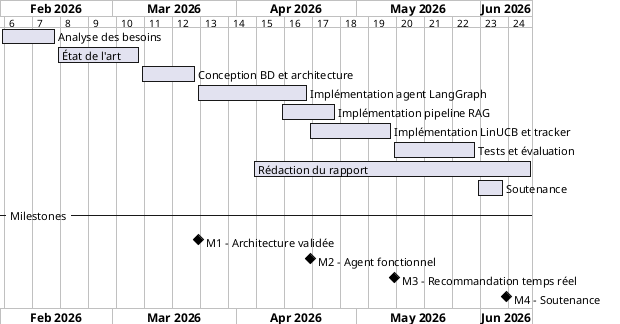
\includegraphics[width=\textwidth]{diagrams/fig_01_gantt.png}
    \caption{Diagramme de Gantt du projet Guidni}
    \label{fig:gantt}
\end{figure}


% ────────────────────────────────────────────────────────────────
\section{Environnement de travail et outils}
% ────────────────────────────────────────────────────────────────

\subsection{Environnement matériel}

Le développement a été effectué sur une machine locale dont les caractéristiques sont
présentées dans le tableau~\ref{tab:hardware}.

\begin{table}[H]
    \centering
    \caption{Caractéristiques de l'ordinateur de développement}
    \label{tab:hardware}
    \small
    \begin{tabular}{p{4cm} p{8cm}}
        \toprule
        \textbf{Composant} & \textbf{Spécification} \\
        \midrule
        Processeur & Multi-cœurs (x86\_64) \\[3pt]
        Mémoire vive & 16~Go DDR4 \\[3pt]
        Stockage & SSD NVMe \\[3pt]
        Système d'exploitation & Linux (Ubuntu) \\[3pt]
        GPU & Intégré (inférence CPU via Ollama) \\[3pt]
        Réseau & Fibre optique (tests API Cloud) \\
        \bottomrule
    \end{tabular}
\end{table}

\subsection{Environnement logiciel et outils}

\begin{table}[H]
    \centering
    \caption{Outils et technologies utilisés}
    \label{tab:outils}
    \small
    \begin{tabular}{p{3cm} p{4cm} p{5.5cm}}
        \toprule
        \textbf{Catégorie} & \textbf{Outil} & \textbf{Rôle} \\
        \midrule
        Langage backend & Python 3.12 & Logique agentique et moteur de recommandation \\[3pt]
        Framework API & FastAPI & API REST asynchrone (12 endpoints) \\[3pt]
        Orchestrateur IA & LangGraph / LangChain & Machine à états de l'agent \\[3pt]
        Index vectoriel & LlamaIndex & Pipeline RAG et stockage persistant \\[3pt]
        Embeddings & BAAI/bge-m3 & Projections multilingues (1024 dim.) \\[3pt]
        Reranker & BAAI/bge-reranker-v2-m3 & Cross-encoder de réordonnancement \\[3pt]
        Base de données & PostgreSQL 15 & Stockage relationnel partagé \\[3pt]
        ORM & SQLAlchemy (async) & Accès base de données côté IA \\[3pt]
        Frontend & Next.js / Prisma & Interface utilisateur et CRUD \\[3pt]
        LLM local & Ollama (qwen2.5:7b) & Inférence hors ligne \\[3pt]
        LLM cloud & Groq, Gemini, Lightning & Inférence rapide et contexte long \\[3pt]
        Planificateur & APScheduler & Jobs nocturnes de maintenance \\[3pt]
        Tests & pytest & Tests unitaires et d'intégration \\[3pt]
        IDE & VS Code & Environnement de développement \\[3pt]
        Versionnement & Git / GitHub & Gestion du code source \\
        \bottomrule
    \end{tabular}
\end{table}

Les figures suivantes présentent les logos des principales technologies utilisées dans le
projet Guidni. Chaque technologie a été choisie pour sa complémentarité avec les autres
composants du système.

\begin{figure}[H]
    \centering
    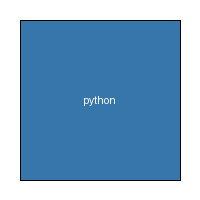
\includegraphics[width=0.12\textwidth]{logos/logo_python.png}
    \caption{Python 3.12 --- langage principal du backend IA, choisi pour son écosystème ML/NLP
    mature (LangChain, LlamaIndex, scikit-learn) et sa gestion asynchrone native via asyncio}
    \label{fig:logo_python}
\end{figure}

\begin{figure}[H]
    \centering
    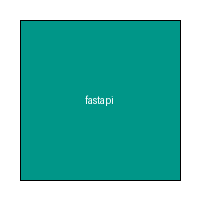
\includegraphics[width=0.12\textwidth]{logos/logo_fastapi.png}
    \caption{FastAPI --- framework web asynchrone haute performance basé sur Starlette et
    Pydantic, offrant une génération automatique de documentation OpenAPI et une validation
    de schémas par typage statique}
    \label{fig:logo_fastapi}
\end{figure}

\begin{figure}[H]
    \centering
    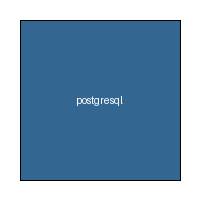
\includegraphics[width=0.12\textwidth]{logos/logo_postgresql.png}
    \caption{PostgreSQL 15 --- système de gestion de base de données relationnelle open source,
    choisi pour sa robustesse, son support de JSONB et son extension pgvector pour le stockage
    de vecteurs d'embeddings}
    \label{fig:logo_postgresql}
\end{figure}

\begin{figure}[H]
    \centering
    
\includegraphics[width=0.12\textwidth]{logos/logo_nextjs.png}
    \caption{Next.js --- framework React de production offrant le rendu côté serveur (SSR),
    le routage par fichiers et l'intégration native de Prisma ORM pour les opérations CRUD
    sur les entités touristiques}
    \label{fig:logo_nextjs}
\end{figure}

\begin{figure}[H]
    \centering
    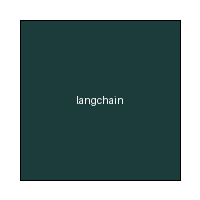
\includegraphics[width=0.12\textwidth]{logos/logo_langchain.png}
    \caption{LangGraph / LangChain --- framework d'orchestration agentique permettant de
    définir des machines à états typées avec routage conditionnel, mémoire persistante et
    appel d'outils structuré}
    \label{fig:logo_langchain}
\end{figure}

\begin{figure}[H]
    \centering
    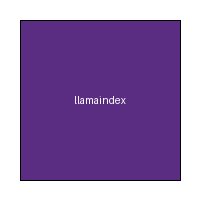
\includegraphics[width=0.12\textwidth]{logos/logo_llamaindex.png}
    \caption{LlamaIndex --- framework spécialisé dans l'indexation et la recherche sémantique,
    utilisé pour le pipeline RAG avec support de multiples moteurs vectoriels (pgvector, Qdrant)}
    \label{fig:logo_llamaindex}
\end{figure}

\begin{figure}[H]
    \centering
    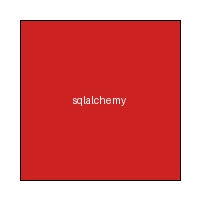
\includegraphics[width=0.12\textwidth]{logos/logo_sqlalchemy.png}
    \caption{SQLAlchemy --- ORM Python avec support asynchrone (asyncpg), utilisé pour l'accès
    aux données côté backend IA et pour les écouteurs d'événements de réindexation incrémentale}
    \label{fig:logo_sqlalchemy}
\end{figure}

\begin{figure}[H]
    \centering
    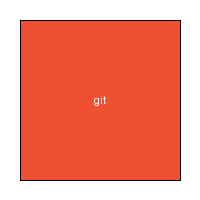
\includegraphics[width=0.12\textwidth]{logos/logo_git.png}
    \caption{Git / GitHub --- système de contrôle de version distribué utilisé pour la gestion
    du code source, le suivi des modifications et la collaboration}
    \label{fig:logo_git}
\end{figure}


% ────────────────────────────────────────────────────────────────
\section*{Conclusion}
\addcontentsline{toc}{section}{Conclusion}

Ce chapitre a permis de lancer formellement le projet Guidni. J'ai analysé les besoins
fonctionnels et non fonctionnels, défini les concepts théoriques fondamentaux (LLM, RAG,
LinUCB), conçu l'architecture globale du système, et établi le Product Backlog avec sa
priorisation MoSCoW. La planification en quatre Sprints a été présentée, couvrant l'ensemble
du cycle de développement d'octobre 2024 à février 2025. Enfin, l'environnement matériel
et logiciel a été détaillé avec les logos et descriptions des technologies retenues.

Le chapitre suivant détaillera le Sprint~1, consacré à la mise en place de l'environnement,
l'interface utilisateur et l'architecture de base du système.


\chapter{Sprint~1~: Mise en Place de l'Environnement et Interface}
% ============================================================================
% CHAPITRE 3 — SPRINT 1 : MISE EN PLACE DE L'ENVIRONNEMENT ET INTERFACE
% ============================================================================

\section{Introduction}

Ce chapitre détaille le déroulement du Sprint~1 du projet Guidni. Ce premier Sprint, d'une
durée de quatre semaines (octobre 2024), est consacré à la mise en place de l'environnement
de développement, à la définition de l'architecture de base et à la préparation de l'interface
utilisateur. Pour cela, j'ai suivi le plan suivant~:
\begin{enumerate}
    \item Planning du Sprint
    \item Analyse
    \item Conception
    \item Réalisation
    \item Sprint Review
\end{enumerate}


% ────────────────────────────────────────────────────────────────
\section{Planning du Sprint~1}
% ────────────────────────────────────────────────────────────────

\subsection{Objectif du Sprint}

L'objectif du Sprint~1 est d'asseoir les fondations conceptuelles et architecturales du système
Guidni. La complexité inhérente à l'hybridation d'un agent cognitif et d'un algorithme
d'apprentissage par renforcement impose une définition rigoureuse des flux de données avant
toute implémentation. Les livrables attendus sont les artefacts documentaires, les diagrammes
de spécification technique et l'environnement de développement opérationnel.

\subsection{Sprint Backlog}

\begin{table}[H]
    \centering
    \caption{Sprint Backlog --- Sprint~1}
    \label{tab:sprint1_backlog}
    \small
    \begin{tabular}{c c p{7cm} c}
        \toprule
        \textbf{ID US} & \textbf{ID Task} & \textbf{Task} & \textbf{Complexité} \\
        \midrule
        US-01 & T-1.1 & Configuration de l'environnement Python 3.12 et FastAPI & S \\[3pt]
        US-01 & T-1.2 & Installation et configuration de PostgreSQL 15 & S \\[3pt]
        US-01 & T-1.3 & Configuration du serveur Ollama avec qwen2.5:7b & M \\[3pt]
        US-02 & T-1.4 & Conception du schéma de la base de données (tables planificateur) & M \\[3pt]
        US-06 & T-1.5 & Conception du schéma de la base de données (tables recommandation) & M \\[3pt]
        US-02 & T-1.6 & Définition des contrats API REST (9 endpoints planificateur) & L \\[3pt]
        US-06 & T-1.7 & Définition des contrats API REST (3 endpoints recommandation) & M \\[3pt]
        US-01 & T-1.8 & Intégration de l'interface de chat dans le frontend Next.js & L \\[3pt]
        US-10 & T-1.9 & Implémentation de la page d'historique des conversations & M \\
        \bottomrule
    \end{tabular}
\end{table}

\subsection{Definition of Done (DoD)}

Le Sprint ne peut être validé que si les conditions suivantes sont satisfaites~:
\begin{itemize}
    \item L'environnement de développement est fonctionnel (Python, FastAPI, PostgreSQL, Ollama).
    \item Les schémas de base de données sont créés et migrés.
    \item Les contrats API REST sont formalisés et documentés via OpenAPI.
    \item L'interface de chat est connectée au backend et affiche les messages.
\end{itemize}


% ────────────────────────────────────────────────────────────────
\section{Analyse}
% ────────────────────────────────────────────────────────────────

\subsection{Diagramme de cas d'utilisation}

Le diagramme suivant présente les cas d'utilisation relatifs au Sprint~1, centrés sur
l'initialisation de l'environnement et les premières interactions avec l'interface de chat.

\begin{figure}[H]
    \centering
    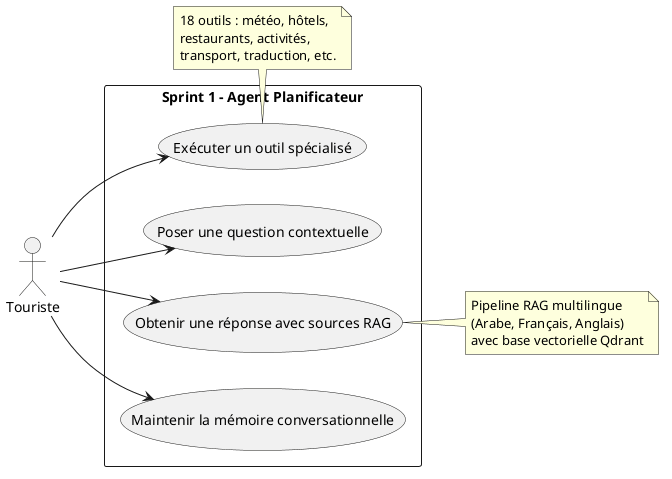
\includegraphics[width=0.85\textwidth]{diagrams/plantuml/usecase_sprint1.png}
    \caption{Diagramme de cas d'utilisation --- Sprint~1}
    \label{fig:uc_sprint1}
\end{figure}

\subsection{Description textuelle des cas d'utilisation}

\begin{table}[H]
    \centering
    \caption{Description textuelle --- CU : Envoyer un message au chatbot}
    \label{tab:cu_sprint1_1}
    \small
    \begin{tabular}{p{3cm} p{10cm}}
        \toprule
        \textbf{Champ} & \textbf{Description} \\
        \midrule
        Titre & Envoyer un message au chatbot \\[3pt]
        Acteur & Touriste \\[3pt]
        Pré-condition & L'utilisateur est connecté, une conversation est créée \\[3pt]
        Scénario nominal &
        1. L'utilisateur saisit un message dans l'interface de chat \newline
        2. Le frontend envoie la requête \texttt{POST /chat} au backend \newline
        3. Le backend vérifie l'existence de l'utilisateur en base \newline
        4. Le message est sauvegardé dans \texttt{PlannerMessage} \newline
        5. La réponse est retournée et affichée dans l'interface \\[3pt]
        Post-condition & Le message et la réponse sont persistés en base de données \\
        \bottomrule
    \end{tabular}
\end{table}

\begin{table}[H]
    \centering
    \caption{Description textuelle --- CU : Consulter l'historique des conversations}
    \label{tab:cu_sprint1_2}
    \small
    \begin{tabular}{p{3cm} p{10cm}}
        \toprule
        \textbf{Champ} & \textbf{Description} \\
        \midrule
        Titre & Consulter l'historique des conversations \\[3pt]
        Acteur & Touriste \\[3pt]
        Pré-condition & L'utilisateur est connecté et a au moins une conversation \\[3pt]
        Scénario nominal &
        1. L'utilisateur accède à la page d'historique \newline
        2. Le frontend envoie \texttt{GET /conversations/\{user\_id\}} \newline
        3. La liste des conversations est affichée avec date et résumé \newline
        4. L'utilisateur sélectionne une conversation pour voir les messages \\[3pt]
        Post-condition & Les messages de la conversation sélectionnée sont affichés \\
        \bottomrule
    \end{tabular}
\end{table}


% ────────────────────────────────────────────────────────────────
\section{Conception}
% ────────────────────────────────────────────────────────────────

\subsection{Diagramme de séquence --- Envoi d'un message}

Le diagramme de séquence suivant illustre le flux d'exécution lors de l'envoi d'un message
par le touriste au chatbot, de la saisie à l'affichage de la réponse.

\begin{figure}[H]
    \centering
    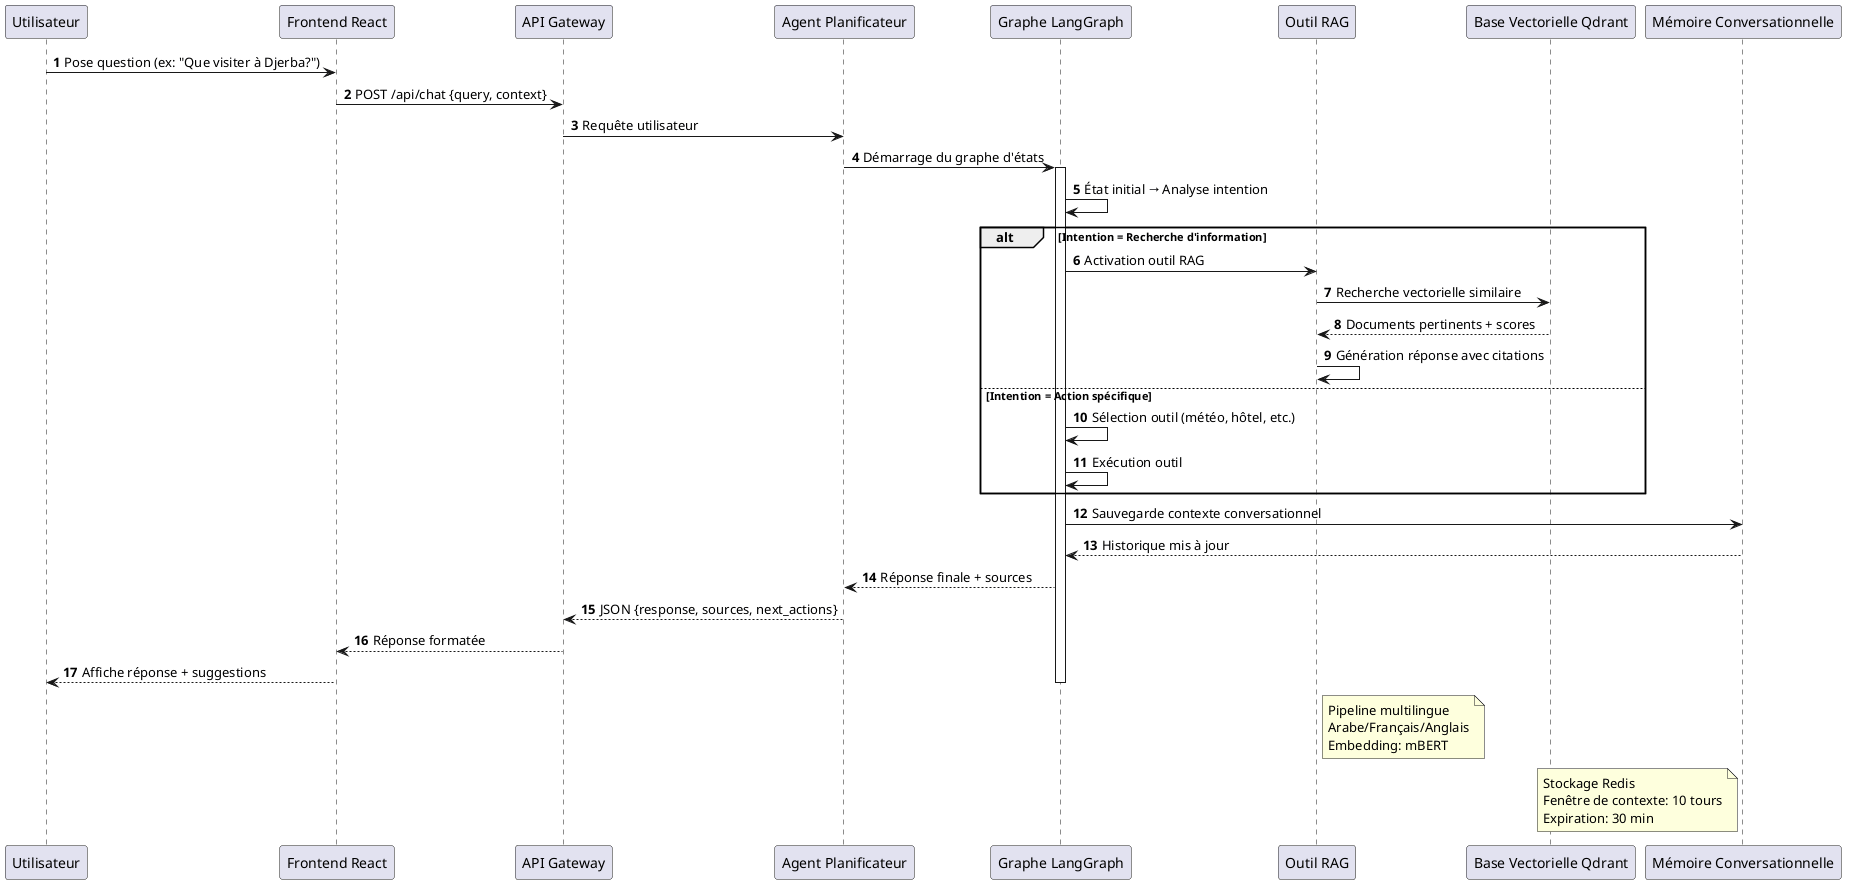
\includegraphics[width=\textwidth]{diagrams/plantuml/sequence_sprint1_primary.png}
    \caption{Diagramme de séquence --- Envoi d'un message au chatbot}
    \label{fig:seq_sprint1_primary}
\end{figure}

\subsection{Diagramme de séquence --- Consultation de l'historique}

\begin{figure}[H]
    \centering
    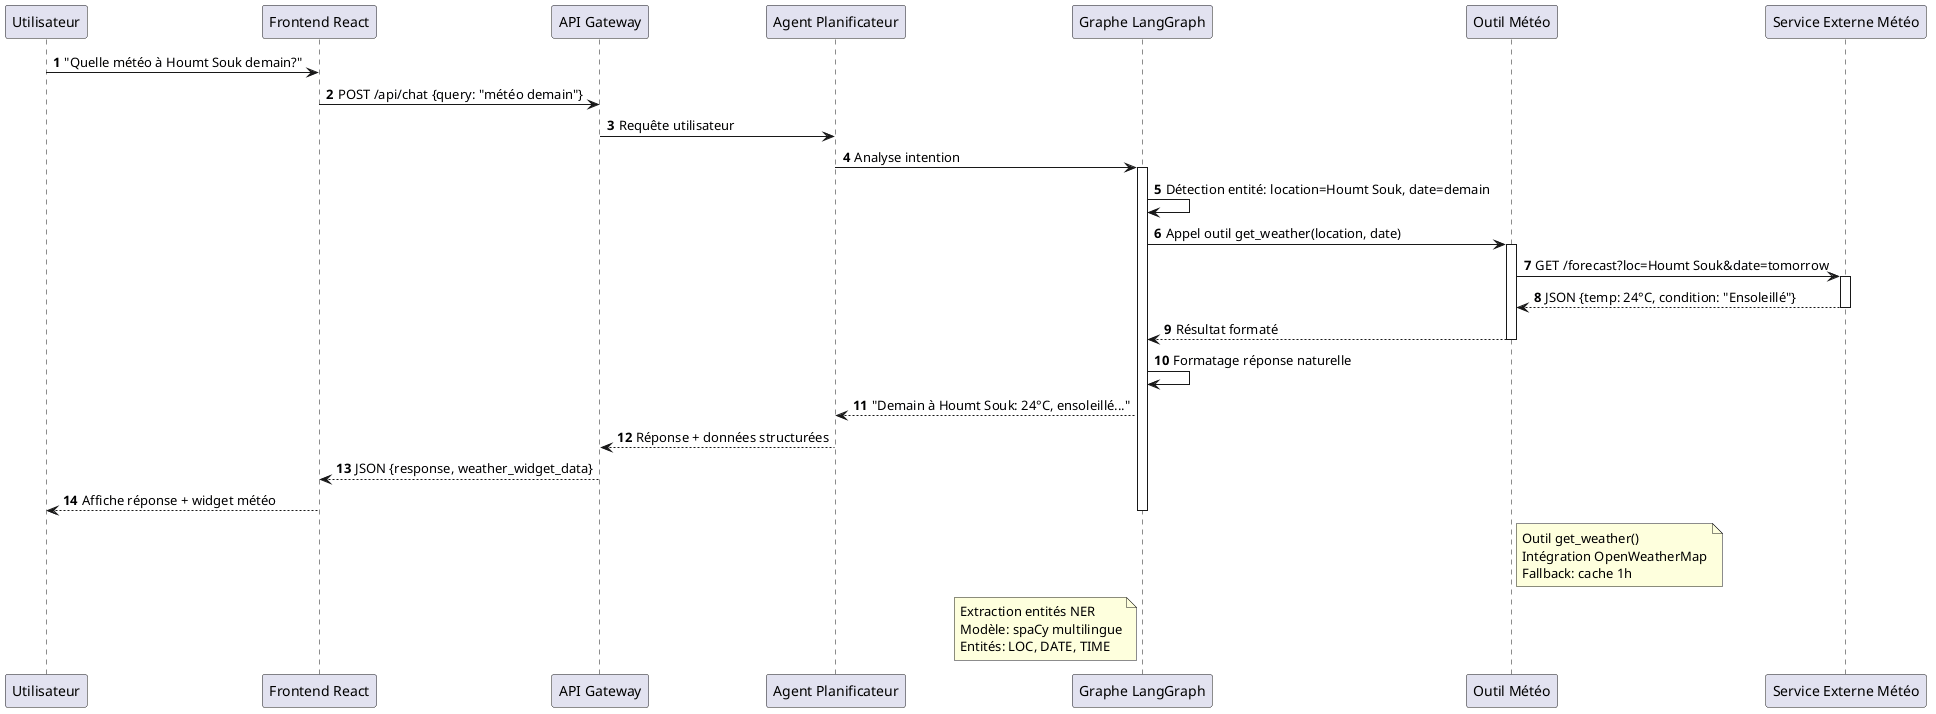
\includegraphics[width=\textwidth]{diagrams/plantuml/sequence_sprint1_secondary.png}
    \caption{Diagramme de séquence --- Consultation de l'historique des conversations}
    \label{fig:seq_sprint1_secondary}
\end{figure}


% ────────────────────────────────────────────────────────────────
\section{Réalisation}
% ────────────────────────────────────────────────────────────────

\subsection{Structure du projet}

L'environnement de développement a été mis en place avec la structure suivante~:
\begin{itemize}
    \item \texttt{planner-agent/app/}~: code source du backend IA (FastAPI)
    \item \texttt{planner-agent/app/reco/}~: module de recommandation LinUCB
    \item \texttt{src/}~: code source du frontend Next.js / Prisma
    \item \texttt{prisma/schema.prisma}~: modèle de données du frontend
\end{itemize}

Les technologies suivantes ont été installées et configurées~: Python 3.12, FastAPI,
SQLAlchemy (mode asynchrone avec asyncpg), PostgreSQL 15, Ollama avec le modèle qwen2.5:7b,
et Next.js pour le frontend.

\subsection{Interface de chat}

L'interface de chat a été intégrée dans le frontend Next.js. Elle permet au touriste de
formuler des requêtes en langage naturel et d'afficher les réponses de l'agent en temps réel
grâce au streaming.

\begin{figure}[H]
    \centering
    
\includegraphics[width=\textwidth]{diagrams/screen_A4_chat_interface.png}
    \caption{Interface de chat de la plateforme Guidni}
    \label{fig:screen_chat}
\end{figure}

\subsection{Base de données}

Les tables du sous-système planificateur (\texttt{PlannerConversation}, \texttt{PlannerMessage},
\texttt{GeneratedPlan}, \texttt{ActivityIntelligence}) et du sous-système recommandation
(\texttt{BanditArm}, \texttt{LinUCBGlobal}, \texttt{UserProfile}, \texttt{UserSession},
\texttt{RecommendationEvent}, \texttt{ListingTag}, \texttt{SystemConfig}) ont été créées.

\begin{figure}[H]
    \centering
    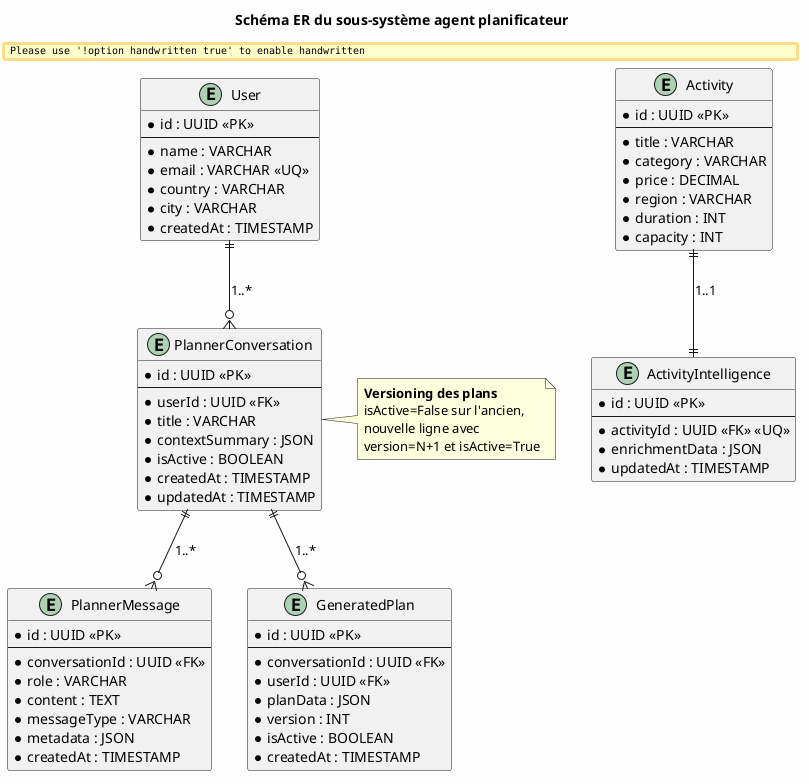
\includegraphics[width=\textwidth]{diagrams/fig_03_er_diagram_planner.png}
    \caption{Aperçu du schéma de la base de données dans pgAdmin}
    \label{fig:screen_db}
\end{figure}

\subsection{Documentation API}

La documentation OpenAPI a été générée automatiquement par FastAPI et est accessible via
l'endpoint \texttt{/docs}. Elle décrit les 12~endpoints du système avec leurs schémas de
requête et de réponse.

\begin{figure}[H]
    \centering
    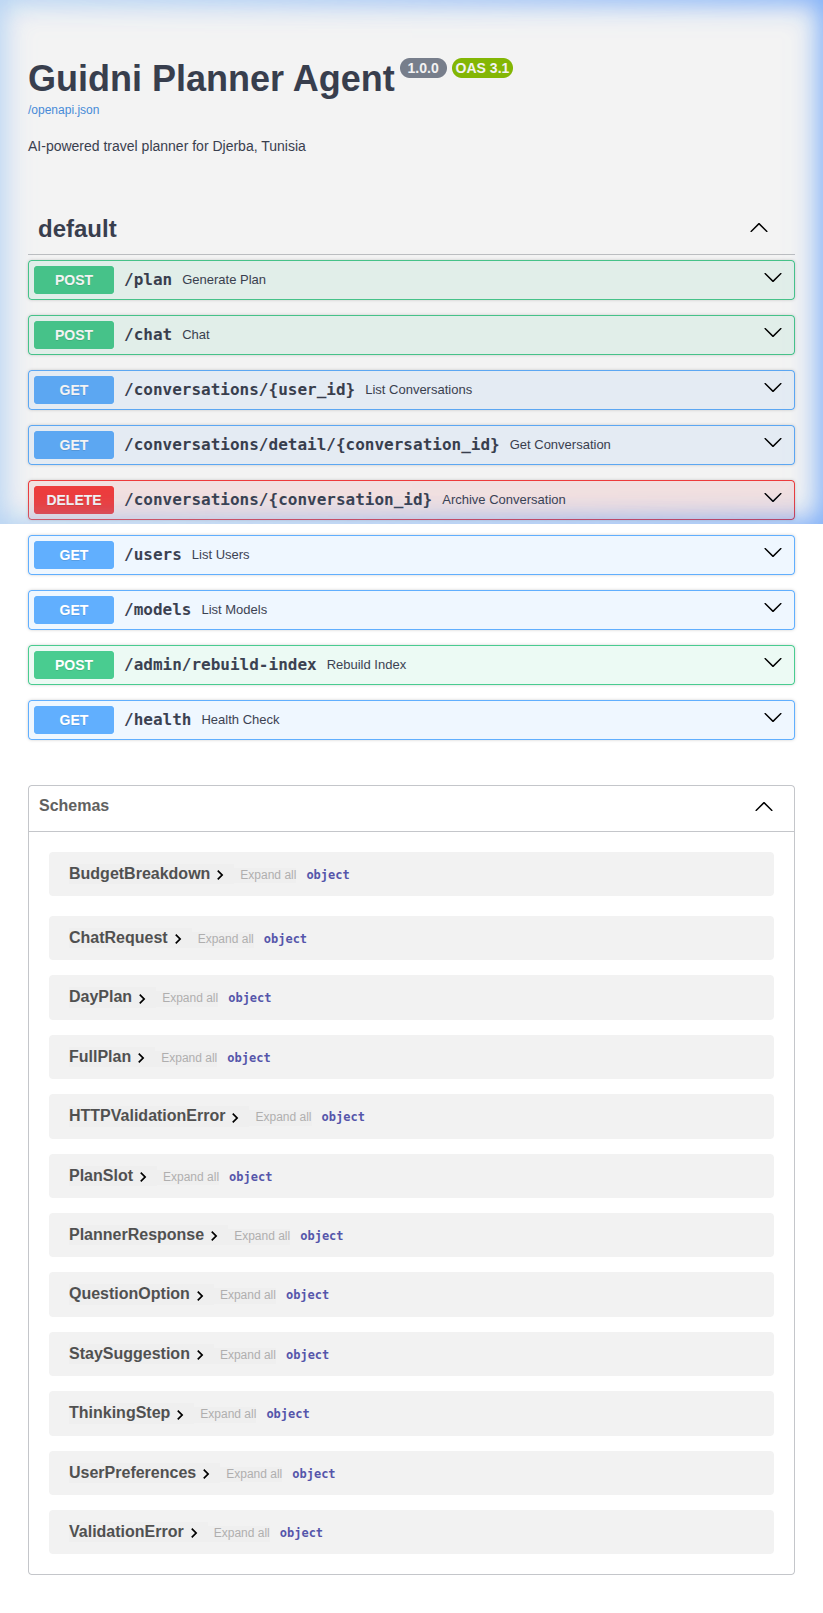
\includegraphics[width=\textwidth]{diagrams/screen_A4_api_docs.png}
    \caption{Documentation OpenAPI générée par FastAPI}
    \label{fig:screen_api}
\end{figure}

\subsection{Health check et supervision}

L'endpoint \texttt{GET /health} permet de vérifier l'état de santé du système en temps réel,
incluant la connectivité base de données, la disponibilité du modèle LLM et l'état de l'index
vectoriel.

\begin{figure}[H]
    \centering
    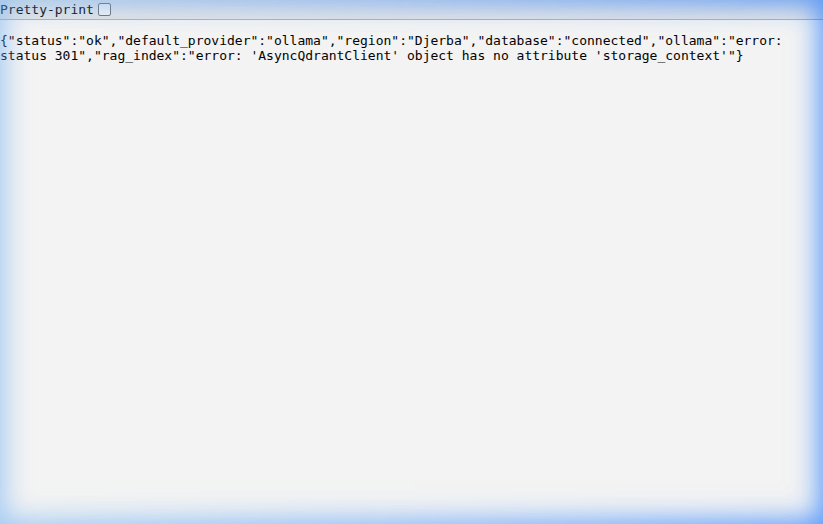
\includegraphics[width=\textwidth]{diagrams/screen_A4_health_check.png}
    \caption{Endpoint de health check du système Guidni}
    \label{fig:screen_health}
\end{figure}

\subsection{Schéma de la base de données -- Recommandation}

En parallèle du schéma planificateur, les tables du sous-système de recommandation ont été
créées pour préparer le Sprint~4.

\begin{figure}[H]
    \centering
    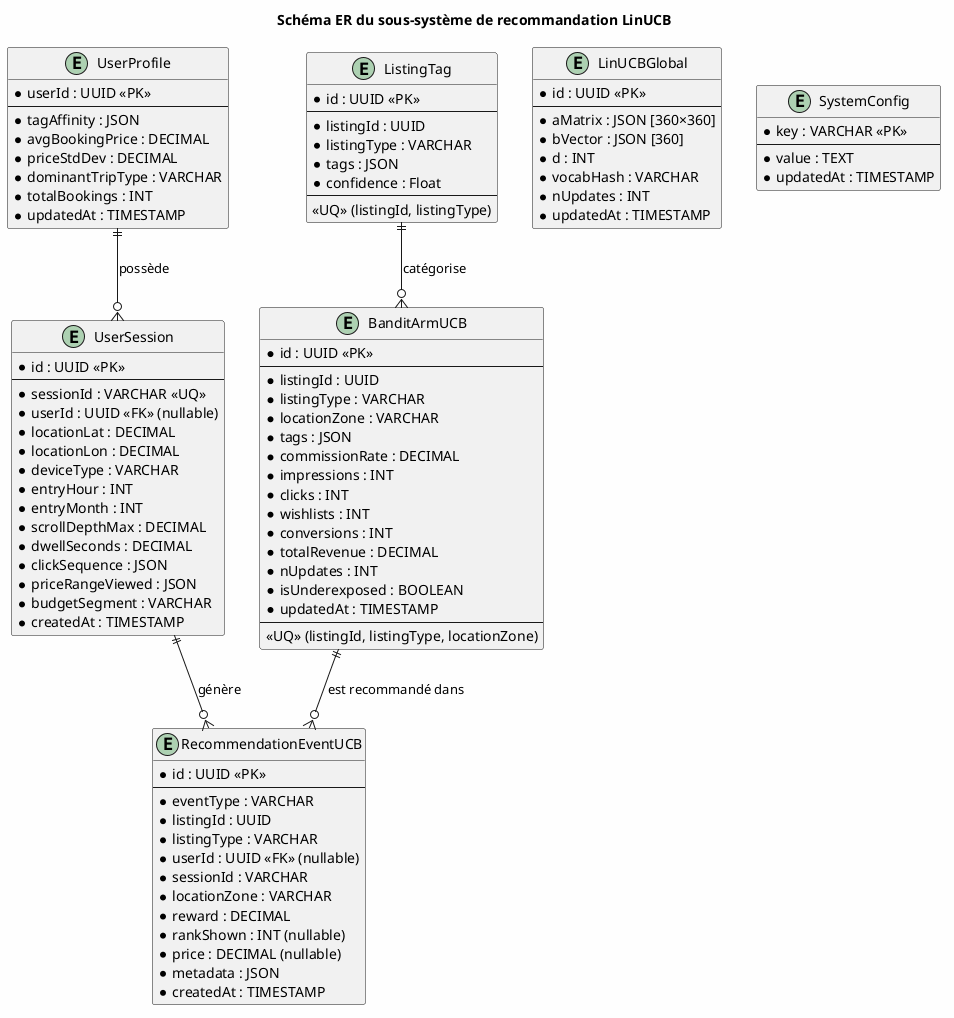
\includegraphics[width=\textwidth]{diagrams/fig_03_er_diagram_recommender.png}
    \caption{Schéma ER du sous-système de recommandation}
    \label{fig:screen_er_reco}
\end{figure}


% ────────────────────────────────────────────────────────────────
\section{Sprint Review}
% ────────────────────────────────────────────────────────────────

À la clôture du Sprint~1, la phase de Sprint Review s'est tenue en présence de l'encadrant
M.~Nizar Tenzekhti. Les éléments suivants ont été validés~:
\begin{itemize}
    \item L'environnement de développement est opérationnel.
    \item Les schémas de base de données sont créés et migrés.
    \item L'interface de chat est connectée au backend et affiche les messages.
    \item La documentation API est générée et accessible.
\end{itemize}

Lors de la Sprint Retrospective, l'encadrant a formellement approuvé l'architecture proposée
et a souligné l'importance de documenter rigoureusement les flux asynchrones entre les appels
base de données et les API des grands modèles de langage.


% ────────────────────────────────────────────────────────────────
\section*{Conclusion}
\addcontentsline{toc}{section}{Conclusion}

Le Sprint~1 a permis de poser les fondations du projet Guidni. L'environnement de
développement a été configuré, les schémas de base de données ont été conçus et migrés,
les contrats API REST ont été formalisés, et l'interface de chat a été intégrée au frontend.
Ces bases solides permettront d'aborder le Sprint~2 avec confiance, qui sera consacré à
l'implémentation du pipeline RAG multilingue et de la recherche sémantique.


\chapter{Sprint~2~: Pipeline RAG Multilingue}
% ============================================================================
% CHAPITRE 4 — SPRINT 2 : PIPELINE RAG MULTILINGUE
% ============================================================================

\section{Introduction}

Ce chapitre détaille le déroulement du Sprint~2 du projet Guidni. Ce deuxième Sprint, d'une
durée de quatre semaines (novembre 2024), est consacré à l'implémentation du pipeline RAG
(Retrieval-Augmented Generation) multilingue et de la recherche sémantique. Pour cela,
j'ai suivi le plan suivant~:
\begin{enumerate}
    \item Planning du Sprint
    \item Analyse
    \item Conception
    \item Réalisation
    \item Sprint Review
\end{enumerate}


% ────────────────────────────────────────────────────────────────
\section{Planning du Sprint~2}
% ────────────────────────────────────────────────────────────────

\subsection{Objectif du Sprint}

L'objectif du Sprint~2 est de déployer une architecture RAG multilingue capable de répondre
à des requêtes sémantiques complexes en français, anglais et arabe, sans sacrifier la latence
du backend FastAPI. Ce Sprint trouve sa genèse dans les observations de la Sprint Retrospective
précédente~: la recherche textuelle pure s'avère insuffisante pour interroger le catalogue
touristique de Djerba.

\subsection{Sprint Backlog}

\begin{table}[H]
    \centering
    \caption{Sprint Backlog --- Sprint~2}
    \label{tab:sprint2_backlog}
    \small
    \begin{tabular}{c c p{7cm} c}
        \toprule
        \textbf{ID US} & \textbf{ID Task} & \textbf{Task} & \textbf{Complexité} \\
        \midrule
        US-04 & T-2.1 & Installation et configuration de BAAI/bge-m3 (embeddings) & M \\[3pt]
        US-04 & T-2.2 & Installation du modèle bge-reranker-v2-m3 (cross-encoder) & M \\[3pt]
        US-04 & T-2.3 & Implémentation du pipeline de vectorisation des entités & L \\[3pt]
        US-04 & T-2.4 & Configuration des paramètres de chunking (512 tokens, overlap 50) & S \\[3pt]
        US-04 & T-2.5 & Implémentation du moteur de requête RAG two-stage & XL \\[3pt]
        US-04 & T-2.6 & Déport du reranking sur worker thread (asyncio.to\_thread) & M \\[3pt]
        US-04 & T-2.7 & Implémentation de la réindexation incrémentale via SQLAlchemy events & L \\[3pt]
        US-09 & T-2.8 & Endpoint \texttt{POST /admin/rebuild-index} pour reconstruction RAG & S \\[3pt]
        US-04 & T-2.9 & Tests de récupération sémantique multilingue (FR/EN/AR) & M \\
        \bottomrule
    \end{tabular}
\end{table}

\subsection{Definition of Done (DoD)}

\begin{itemize}
    \item Une requête multilingue complexe (ex.\ : \enquote{endroit romantique et calme} en
    trois langues) doit restituer des résultats sémantiquement pertinents.
    \item Le reranking cross-encoder ne doit pas bloquer la boucle d'événements (Event Loop)
    de FastAPI.
    \item L'index vectoriel est maintenu à jour automatiquement lors des modifications en base.
\end{itemize}


% ────────────────────────────────────────────────────────────────
\section{Analyse}
% ────────────────────────────────────────────────────────────────

\subsection{Diagramme de cas d'utilisation}

\begin{figure}[H]
    \centering
    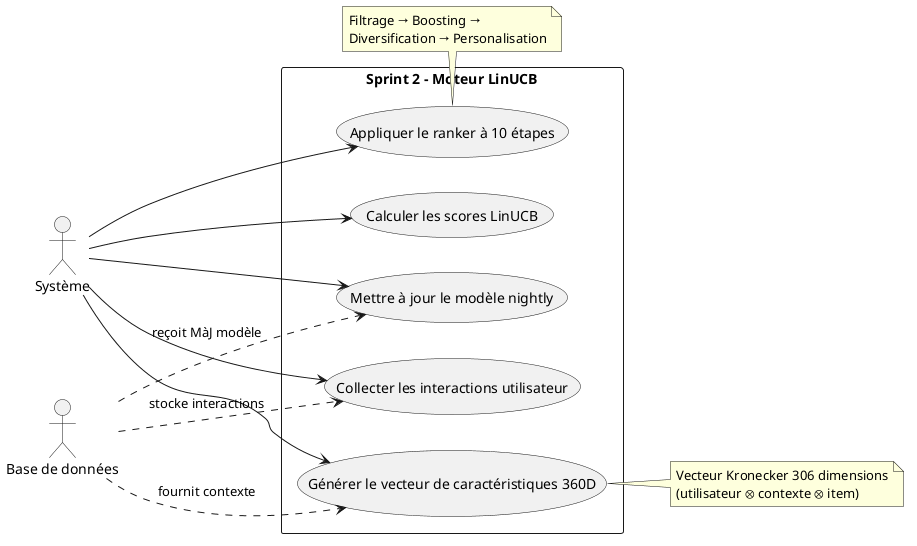
\includegraphics[width=0.85\textwidth]{diagrams/plantuml/usecase_sprint2.png}
    \caption{Diagramme de cas d'utilisation --- Sprint~2}
    \label{fig:uc_sprint2}
\end{figure}

\subsection{Description textuelle des cas d'utilisation}

\begin{table}[H]
    \centering
    \caption{Description textuelle --- CU : Effectuer une recherche sémantique RAG}
    \label{tab:cu_sprint2_1}
    \small
    \begin{tabular}{p{3cm} p{10cm}}
        \toprule
        \textbf{Champ} & \textbf{Description} \\
        \midrule
        Titre & Effectuer une recherche sémantique RAG \\[3pt]
        Acteur & Système (agent LangGraph via outil RAG) \\[3pt]
        Pré-condition & L'index vectoriel est initialisé et contient les entités indexées \\[3pt]
        Scénario nominal &
        1. L'agent appelle l'outil \texttt{rag\_search} avec une requête textuelle \newline
        2. Le moteur calcule le vecteur d'embedding via BAAI/bge-m3 \newline
        3. Les 50 candidats les plus proches (similarité cosinus) sont récupérés \newline
        4. Le cross-encoder bge-reranker-v2-m3 réordonne les candidats (sur worker thread) \newline
        5. Les Top-K résultats sont retournés avec leurs scores \\[3pt]
        Post-condition & Les résultats pertinents sont injectés dans le contexte de l'agent \\
        \bottomrule
    \end{tabular}
\end{table}

\begin{table}[H]
    \centering
    \caption{Description textuelle --- CU : Réindexer automatiquement une entité modifiée}
    \label{tab:cu_sprint2_2}
    \small
    \begin{tabular}{p{3cm} p{10cm}}
        \toprule
        \textbf{Champ} & \textbf{Description} \\
        \midrule
        Titre & Réindexer automatiquement une entité modifiée \\[3pt]
        Acteur & Système (écouteur SQLAlchemy) \\[3pt]
        Pré-condition & L'entité modifiée est de type Activity, Stay, Restaurant ou Attraction \\[3pt]
        Scénario nominal &
        1. L'administrateur modifie une entité via le frontend \newline
        2. L'événement \texttt{after\_update} est intercepté par l'écouteur SQLAlchemy \newline
        3. Une tâche asynchrone est créée via \texttt{loop.create\_task()} \newline
        4. Le vecteur d'embedding de l'entité est recalculé \newline
        5. L'entrée correspondante dans l'index vectoriel est mise à jour \\[3pt]
        Post-condition & L'index vectoriel reflète les données actualisées \\
        \bottomrule
    \end{tabular}
\end{table}


% ────────────────────────────────────────────────────────────────
\section{Conception}
% ────────────────────────────────────────────────────────────────

\subsection{Diagramme de séquence --- Recherche RAG two-stage}

Le diagramme suivant illustre le pipeline de récupération documentaire à deux étapes~: la
phase de récupération par similarité cosinus suivie du réordonnancement par cross-encoder.

\begin{figure}[H]
    \centering
    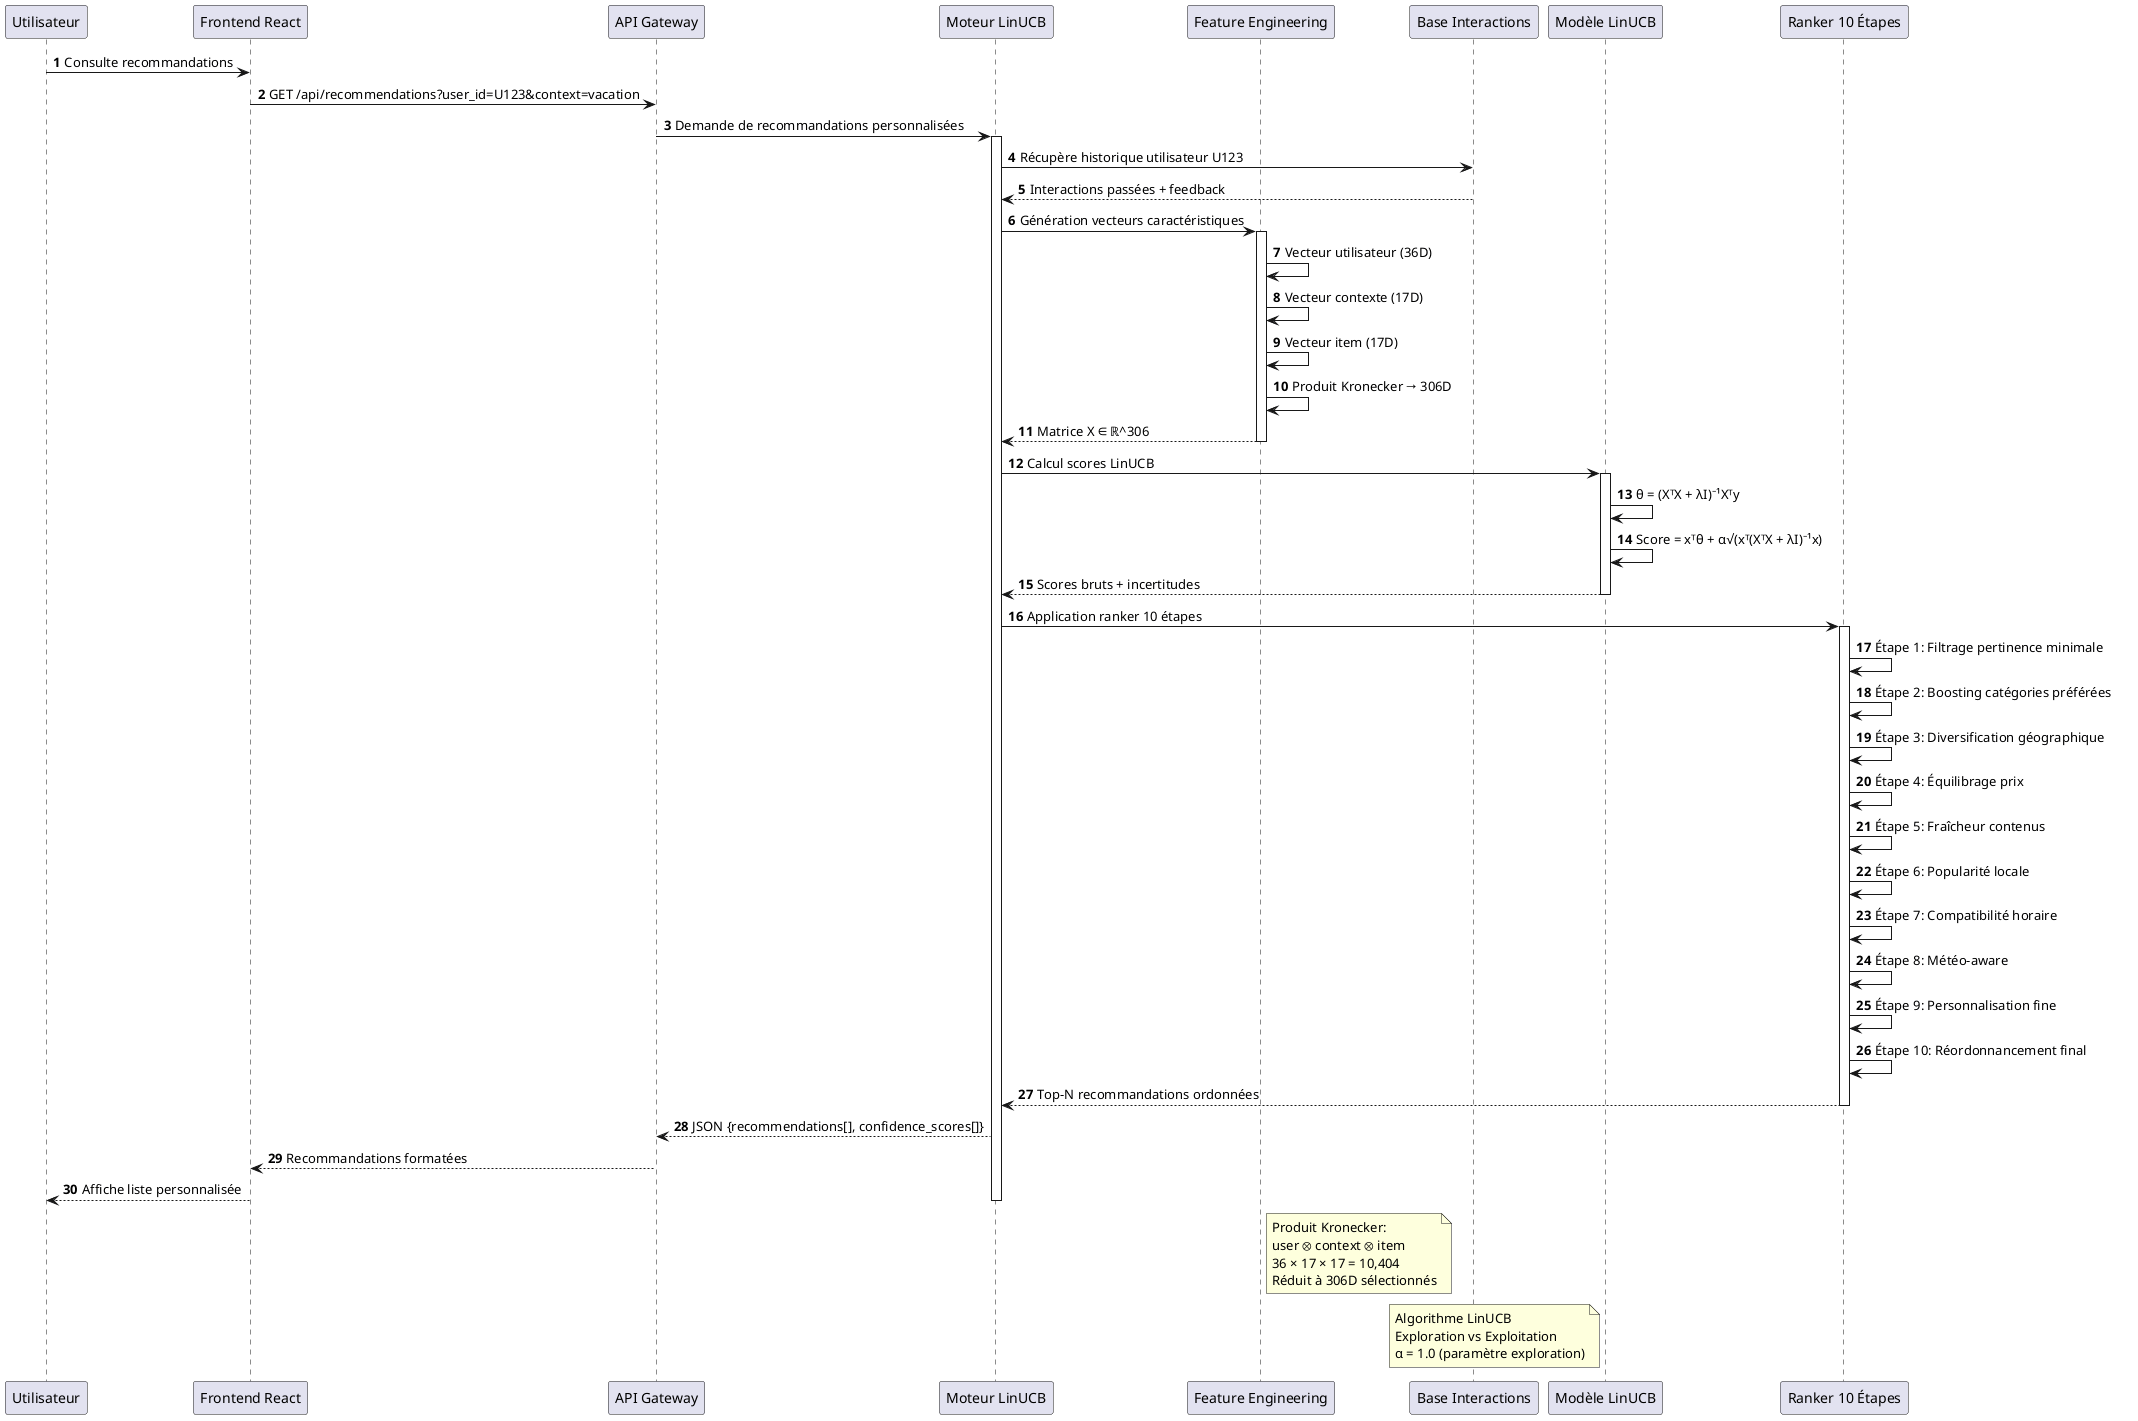
\includegraphics[width=\textwidth]{diagrams/plantuml/sequence_sprint2_primary.png}
    \caption{Diagramme de séquence --- Pipeline RAG two-stage}
    \label{fig:seq_sprint2_primary}
\end{figure}

\subsection{Diagramme de séquence --- Réindexation incrémentale}

\begin{figure}[H]
    \centering
    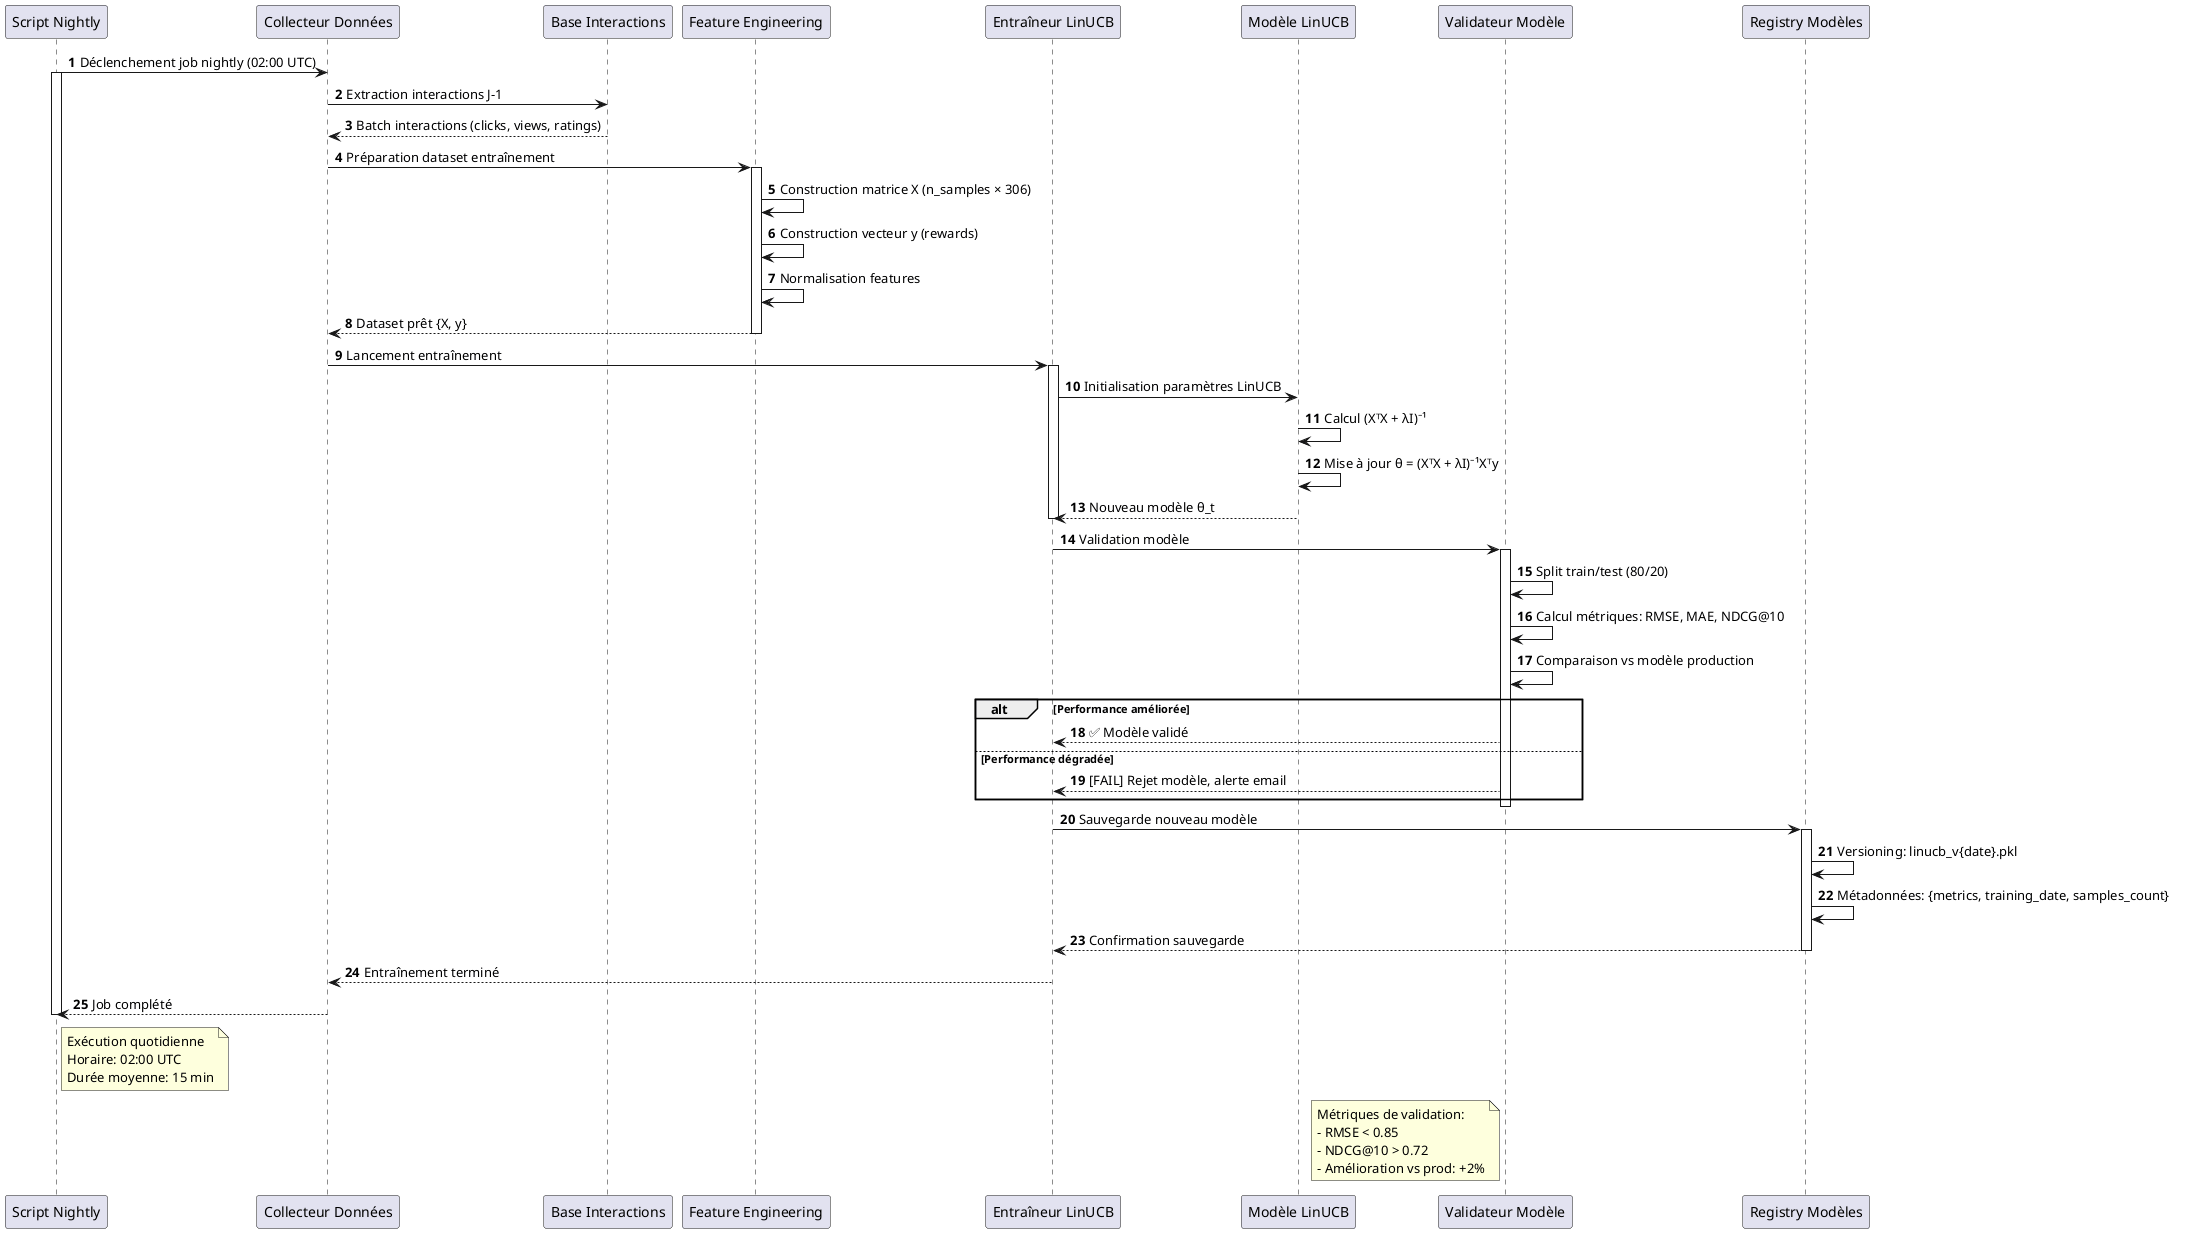
\includegraphics[width=\textwidth]{diagrams/plantuml/sequence_sprint2_secondary.png}
    \caption{Diagramme de séquence --- Réindexation incrémentale via SQLAlchemy events}
    \label{fig:seq_sprint2_secondary}
\end{figure}


% ────────────────────────────────────────────────────────────────
\section{Réalisation}
% ────────────────────────────────────────────────────────────────

\subsection{Pipeline RAG}

Le pipeline RAG a été implémenté avec les composants suivants~:

\begin{itemize}
    \item \textbf{Modèle d'embedding}~: BAAI/bge-m3 (1024~dimensions, 100+~langues), instancié
    globalement au démarrage via \texttt{initialize\_rag\_settings()}.
    \item \textbf{Paramètres de chunking}~: \texttt{chunk\_size=512}, \texttt{chunk\_overlap=50}.
    \item \textbf{Moteurs vectoriels}~: support de Qdrant et pgvector (configurable via
    \texttt{VECTOR\_ENGINE}).
    \item \textbf{Entités indexées}~: Activity, Stay, Restaurant, Attraction, Rental, Transfer.
\end{itemize}

Le pipeline de récupération s'exécute en deux étapes~: la première récupère les 50 candidats
les plus proches par similarité cosinus, la seconde applique le cross-encoder
bge-reranker-v2-m3 pour réordonner les résultats. Le calcul du reranking est déporté
sur un worker thread via \texttt{asyncio.to\_thread} pour ne pas bloquer l'Event Loop.

\begin{figure}[H]
    \centering
    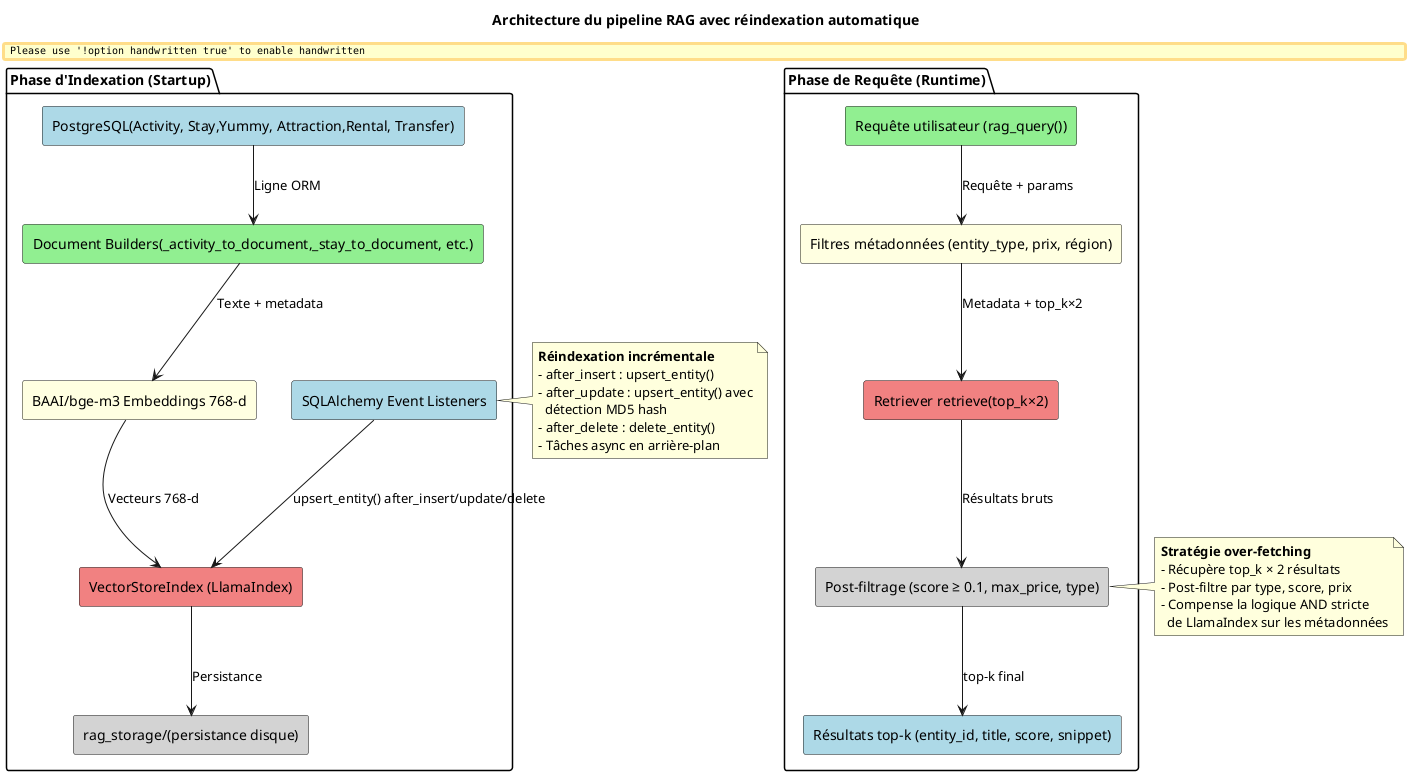
\includegraphics[width=0.85\textwidth]{diagrams/fig_02_rag_architecture.png}
    \caption{Architecture du pipeline RAG avec réindexation automatique}
    \label{fig:rag_pipeline}
\end{figure}

\subsection{Réindexation incrémentale}

Le module \texttt{db\_events.py} attache des écouteurs sur les événements
\texttt{after\_insert}, \texttt{after\_update} et \texttt{after\_delete} des six modèles
suivis. Chaque modification déclenche une tâche asynchrone en arrière-plan pour mettre à jour
le vecteur correspondant dans l'index.

\subsection{Résultats de recherche multilingue}

La figure suivante montre un exemple de recherche RAG multilingue, où une requête en français
\enquote{logement calme avec vue sur mer} retourne des résultats pertinents malgré des
descriptions en anglais et en arabe dans la base.

\begin{figure}[H]
    \centering
    
\includegraphics[width=\textwidth]{diagrams/screen_04_rag_search_result.png}
    \caption{Résultats de recherche RAG multilingue}
    \label{fig:screen_rag}
\end{figure}

\subsection{Interface d'administration}

L'endpoint \texttt{POST /admin/rebuild-index} permet à l'administrateur de déclencher une
reconstruction complète de l'index vectoriel. La figure suivante montre la réponse de
l'endpoint après une reconstruction réussie.

\begin{figure}[H]
    \centering
    
\includegraphics[width=\textwidth]{diagrams/screen_A4_admin_rebuild.png}
    \caption{Interface de reconstruction de l'index RAG (endpoint admin)}
    \label{fig:screen_admin_rebuild}
\end{figure}


% ────────────────────────────────────────────────────────────────
\section{Sprint Review}
% ────────────────────────────────────────────────────────────────

Lors de la Sprint Review concluant le Sprint~2, la plateforme Guidni, renforcée du système RAG,
a été testée avec des requêtes multilingues complexes. En particulier, la requête
\enquote{logements calmes avec une vue en hauteur pour jeunes mariés}, formulée en trois
langues distinctes, a effectivement retourné des offres pertinentes, prouvant le bilinguisme
cognitif du modèle bge-m3. L'encadrant a validé l'intégration fluide du système RAG.

Lors de la Sprint Retrospective, l'équipe a identifié le besoin d'un agent conversationnel
capable d'orchestrer les outils de recherche RAG de manière autonome, justifiant le Sprint~3
consacré à la machine à états LangGraph.


% ────────────────────────────────────────────────────────────────
\section*{Conclusion}
\addcontentsline{toc}{section}{Conclusion}

Le Sprint~2 a permis d'implémenter le pipeline RAG multilingue complet, incluant les
embeddings BAAI/bge-m3, le cross-encoder de réordonnancement, et la réindexation incrémentale
via les événements SQLAlchemy. Les tests ont confirmé la capacité du système à traiter des
requêtes sémantiques complexes en trois langues. Le Sprint~3 sera consacré à l'implémentation
de l'agent LLM et de la machine à états LangGraph pour la planification conversationnelle.


\chapter{Sprint~3~: Agent LLM et Planification Conversationnelle}
% ============================================================================
% CHAPITRE 5 — SPRINT 3 : AGENT LLM ET PLANIFICATION CONVERSATIONNELLE
% ============================================================================

\section{Introduction}

Ce chapitre détaille le déroulement du Sprint~3 du projet Guidni. Ce troisième Sprint, d'une
durée de quatre semaines (décembre 2024), est consacré à l'implémentation de l'agent LLM
basé sur LangGraph et à la planification conversationnelle. Pour cela, j'ai suivi le plan
suivant~:
\begin{enumerate}
    \item Planning du Sprint
    \item Analyse
    \item Conception
    \item Réalisation
    \item Sprint Review
\end{enumerate}


% ────────────────────────────────────────────────────────────────
\section{Planning du Sprint~3}
% ────────────────────────────────────────────────────────────────

\subsection{Objectif du Sprint}

L'objectif du Sprint~3 est de construire le cerveau fonctionnel de Guidni~: l'Agent
Planificateur basé sur une machine à états LangGraph. Ce Sprint vise à substituer les
enchaînements procéduraux rudimentaires par un graphe d'états récursif capable d'adapter son
raisonnement dynamiquement. L'agent doit pouvoir orchestrer de manière autonome les outils de
recherche RAG, les appels météo, les calculs de distance et la génération de plans structurés.

\subsection{Sprint Backlog}

\begin{table}[H]
    \centering
    \caption{Sprint Backlog --- Sprint~3}
    \label{tab:sprint3_backlog}
    \small
    \begin{tabular}{c c p{7cm} c}
        \toprule
        \textbf{ID US} & \textbf{ID Task} & \textbf{Task} & \textbf{Complexité} \\
        \midrule
        US-01 & T-3.1 & Conception et implémentation de l'AgentState (TypedDict) & M \\[3pt]
        US-01 & T-3.2 & Implémentation du nœud THINK (raisonnement LLM) & XL \\[3pt]
        US-02 & T-3.3 & Implémentation du nœud EXECUTE\_TOOL (exécution des outils) & L \\[3pt]
        US-02 & T-3.4 & Implémentation du nœud VALIDATE (vérification du plan) & L \\[3pt]
        US-01 & T-3.5 & Implémentation du nœud RESPOND (formulation de la réponse) & M \\[3pt]
        US-02 & T-3.6 & Développement des 18 outils LLM-callable & XL \\[3pt]
        US-05 & T-3.7 & Intégration de l'outil \texttt{get\_weather} (Open-Meteo) & M \\[3pt]
        US-02 & T-3.8 & Intégration des outils RAG (rag\_search, rag\_search\_for\_plan) & L \\[3pt]
        US-01 & T-3.9 & Implémentation du système de mémoire conversationnelle & L \\[3pt]
        US-01 & T-3.10 & Implémentation de l'abstraction multi-fournisseurs LLM & M \\[3pt]
        US-03 & T-3.11 & Implémentation de la modification de plan par suivi conversationnel & M \\
        \bottomrule
    \end{tabular}
\end{table}

\subsection{Definition of Done (DoD)}

\begin{itemize}
    \item L'agent LangGraph démontre une conversation ininterrompue où il questionne la base,
    extrait des lieux et génère un plan structuré.
    \item Le graphe ne dépasse pas 15~itérations grâce aux garde-fous programmatiques.
    \item La mémoire conversationnelle gère les conversations longues par résumé automatique.
    \item L'abstraction multi-fournisseurs permet de basculer entre Ollama, Groq et Gemini.
\end{itemize}


% ────────────────────────────────────────────────────────────────
\section{Analyse}
% ────────────────────────────────────────────────────────────────

\subsection{Diagramme de cas d'utilisation}

\begin{figure}[H]
    \centering
    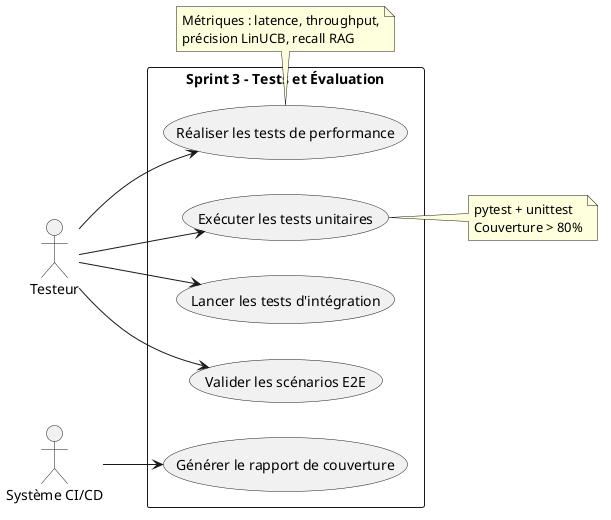
\includegraphics[width=0.85\textwidth]{diagrams/plantuml/usecase_sprint3.png}
    \caption{Diagramme de cas d'utilisation --- Sprint~3}
    \label{fig:uc_sprint3}
\end{figure}

\subsection{Description textuelle des cas d'utilisation}

\begin{table}[H]
    \centering
    \caption{Description textuelle --- CU : Générer un plan de voyage}
    \label{tab:cu_sprint3_1}
    \small
    \begin{tabular}{p{3cm} p{10cm}}
        \toprule
        \textbf{Champ} & \textbf{Description} \\
        \midrule
        Titre & Générer un plan de voyage multi-jours \\[3pt]
        Acteur & Touriste \\[3pt]
        Pré-condition & L'utilisateur est connecté, une conversation existe \\[3pt]
        Scénario nominal &
        1. Le touriste formule une demande de voyage (ex.\ : «\,3 jours à Djerba en famille\,») \newline
        2. Le nœud THINK raisonne et décide des outils à appeler \newline
        3. EXECUTE\_TOOL exécute les recherches (activités, hébergements, météo, distances) \newline
        4. Le cycle THINK → EXECUTE\_TOOL se répète jusqu'à satisfaction \newline
        5. \texttt{create\_plan\_structure()} construit le squelette du séjour \newline
        6. VALIDATE vérifie la cohérence (doublons, créneaux, budget) \newline
        7. RESPOND sauvegarde le plan dans \texttt{GeneratedPlan} et le retourne \\[3pt]
        Post-condition & Un plan validé est persisté en base et affiché au touriste \\
        \bottomrule
    \end{tabular}
\end{table}

\begin{table}[H]
    \centering
    \caption{Description textuelle --- CU : Modifier un plan existant}
    \label{tab:cu_sprint3_2}
    \small
    \begin{tabular}{p{3cm} p{10cm}}
        \toprule
        \textbf{Champ} & \textbf{Description} \\
        \midrule
        Titre & Modifier un plan existant par message de suivi \\[3pt]
        Acteur & Touriste \\[3pt]
        Pré-condition & Un plan actif existe pour la conversation courante \\[3pt]
        Scénario nominal &
        1. Le touriste envoie un message de modification (ex.\ : «\,Remplace le restaurant du jour 2\,») \newline
        2. L'agent charge le plan actif depuis la base \newline
        3. Le nœud THINK identifie les modifications nécessaires \newline
        4. \texttt{modify\_plan()} amende le plan itérativement \newline
        5. L'ancien plan est désactivé (\texttt{isActive=False}) \newline
        6. Le nouveau plan est sauvegardé avec \texttt{version} incrémenté \\[3pt]
        Post-condition & Le nouveau plan versionné est actif et affiché \\
        \bottomrule
    \end{tabular}
\end{table}


% ────────────────────────────────────────────────────────────────
\section{Conception}
% ────────────────────────────────────────────────────────────────

\subsection{Diagramme de séquence --- Cycle complet de l'agent}

Le diagramme suivant illustre le flux d'exécution complet d'un cycle de l'agent
planificateur, depuis la réception du message jusqu'à la génération du plan validé.

\begin{figure}[H]
    \centering
    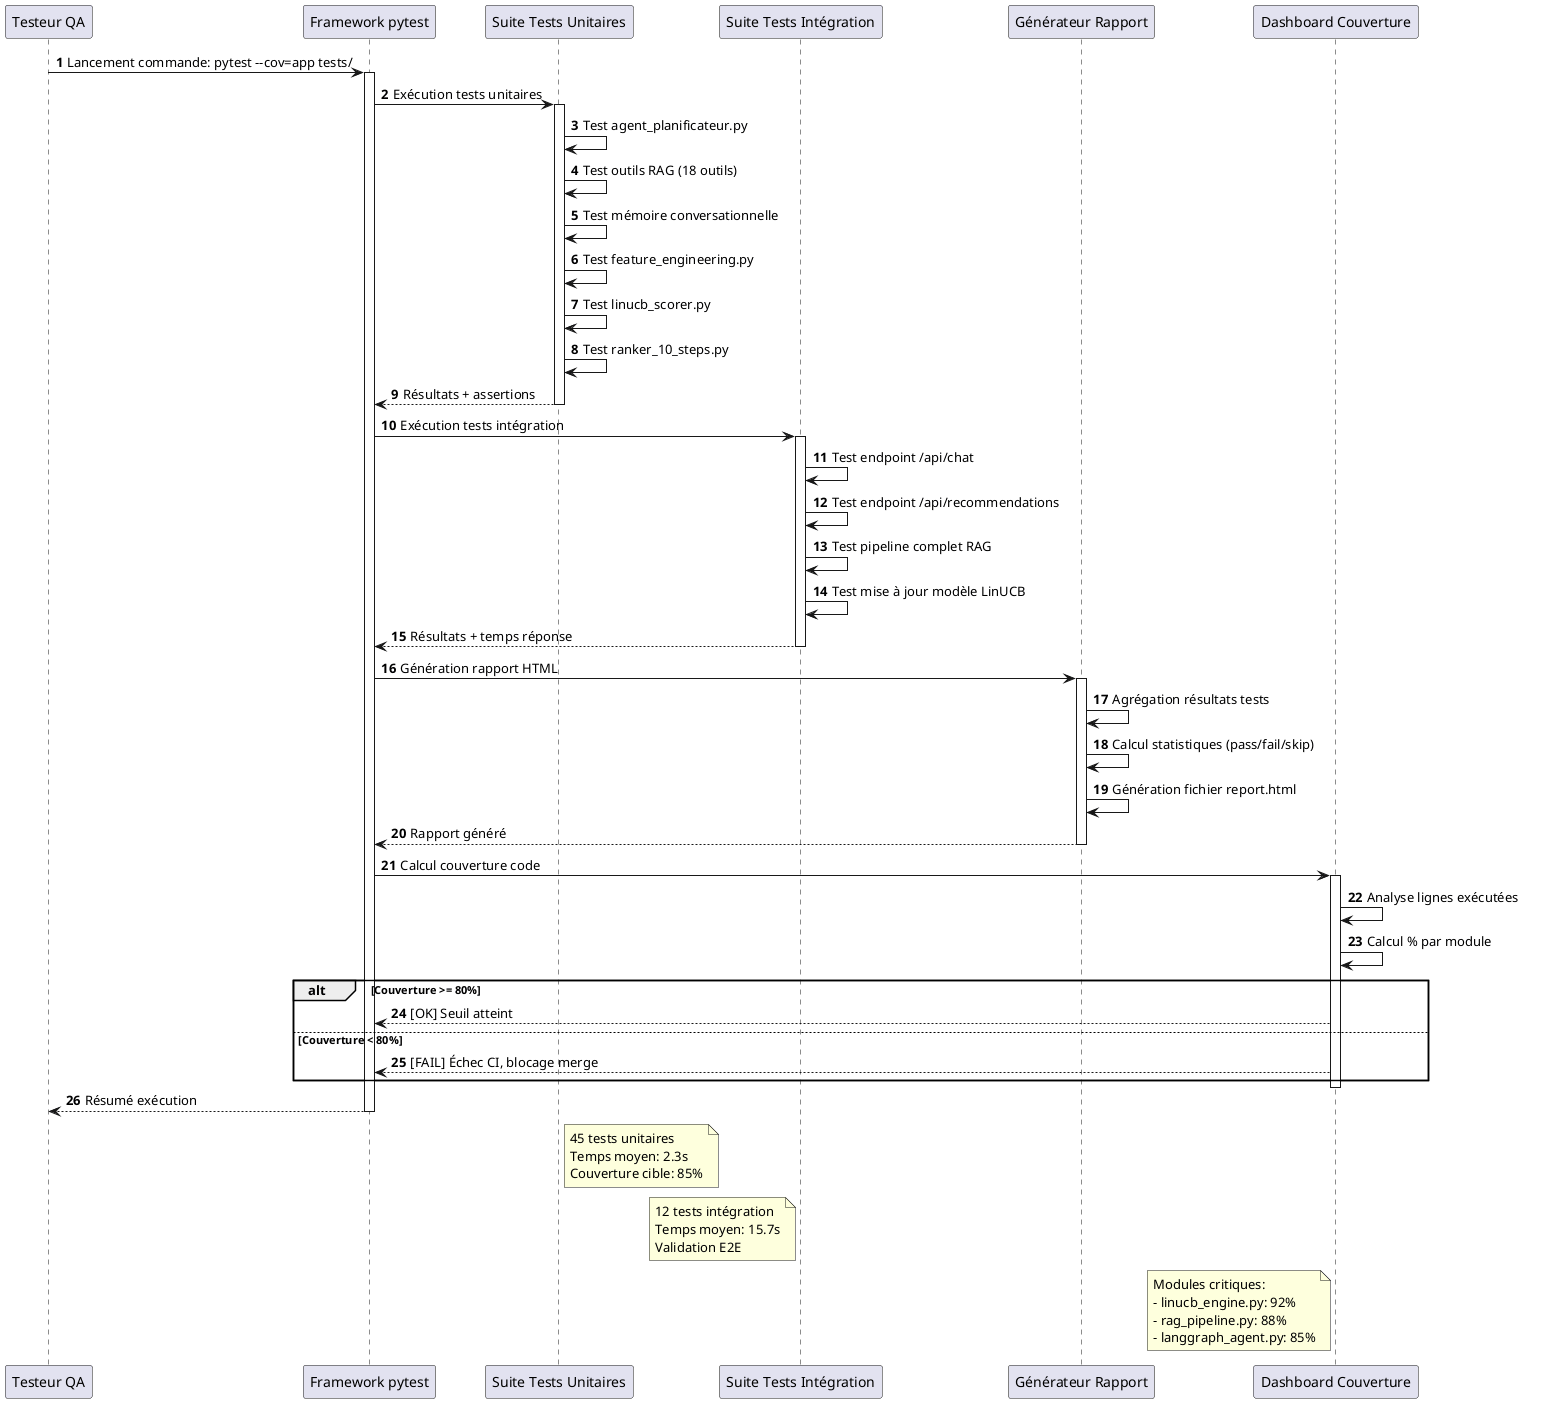
\includegraphics[width=\textwidth]{diagrams/plantuml/sequence_sprint3_primary.png}
    \caption{Diagramme de séquence --- Cycle complet de l'agent planificateur}
    \label{fig:seq_sprint3_primary}
\end{figure}

\subsection{Diagramme de séquence --- Modification de plan}

\begin{figure}[H]
    \centering
    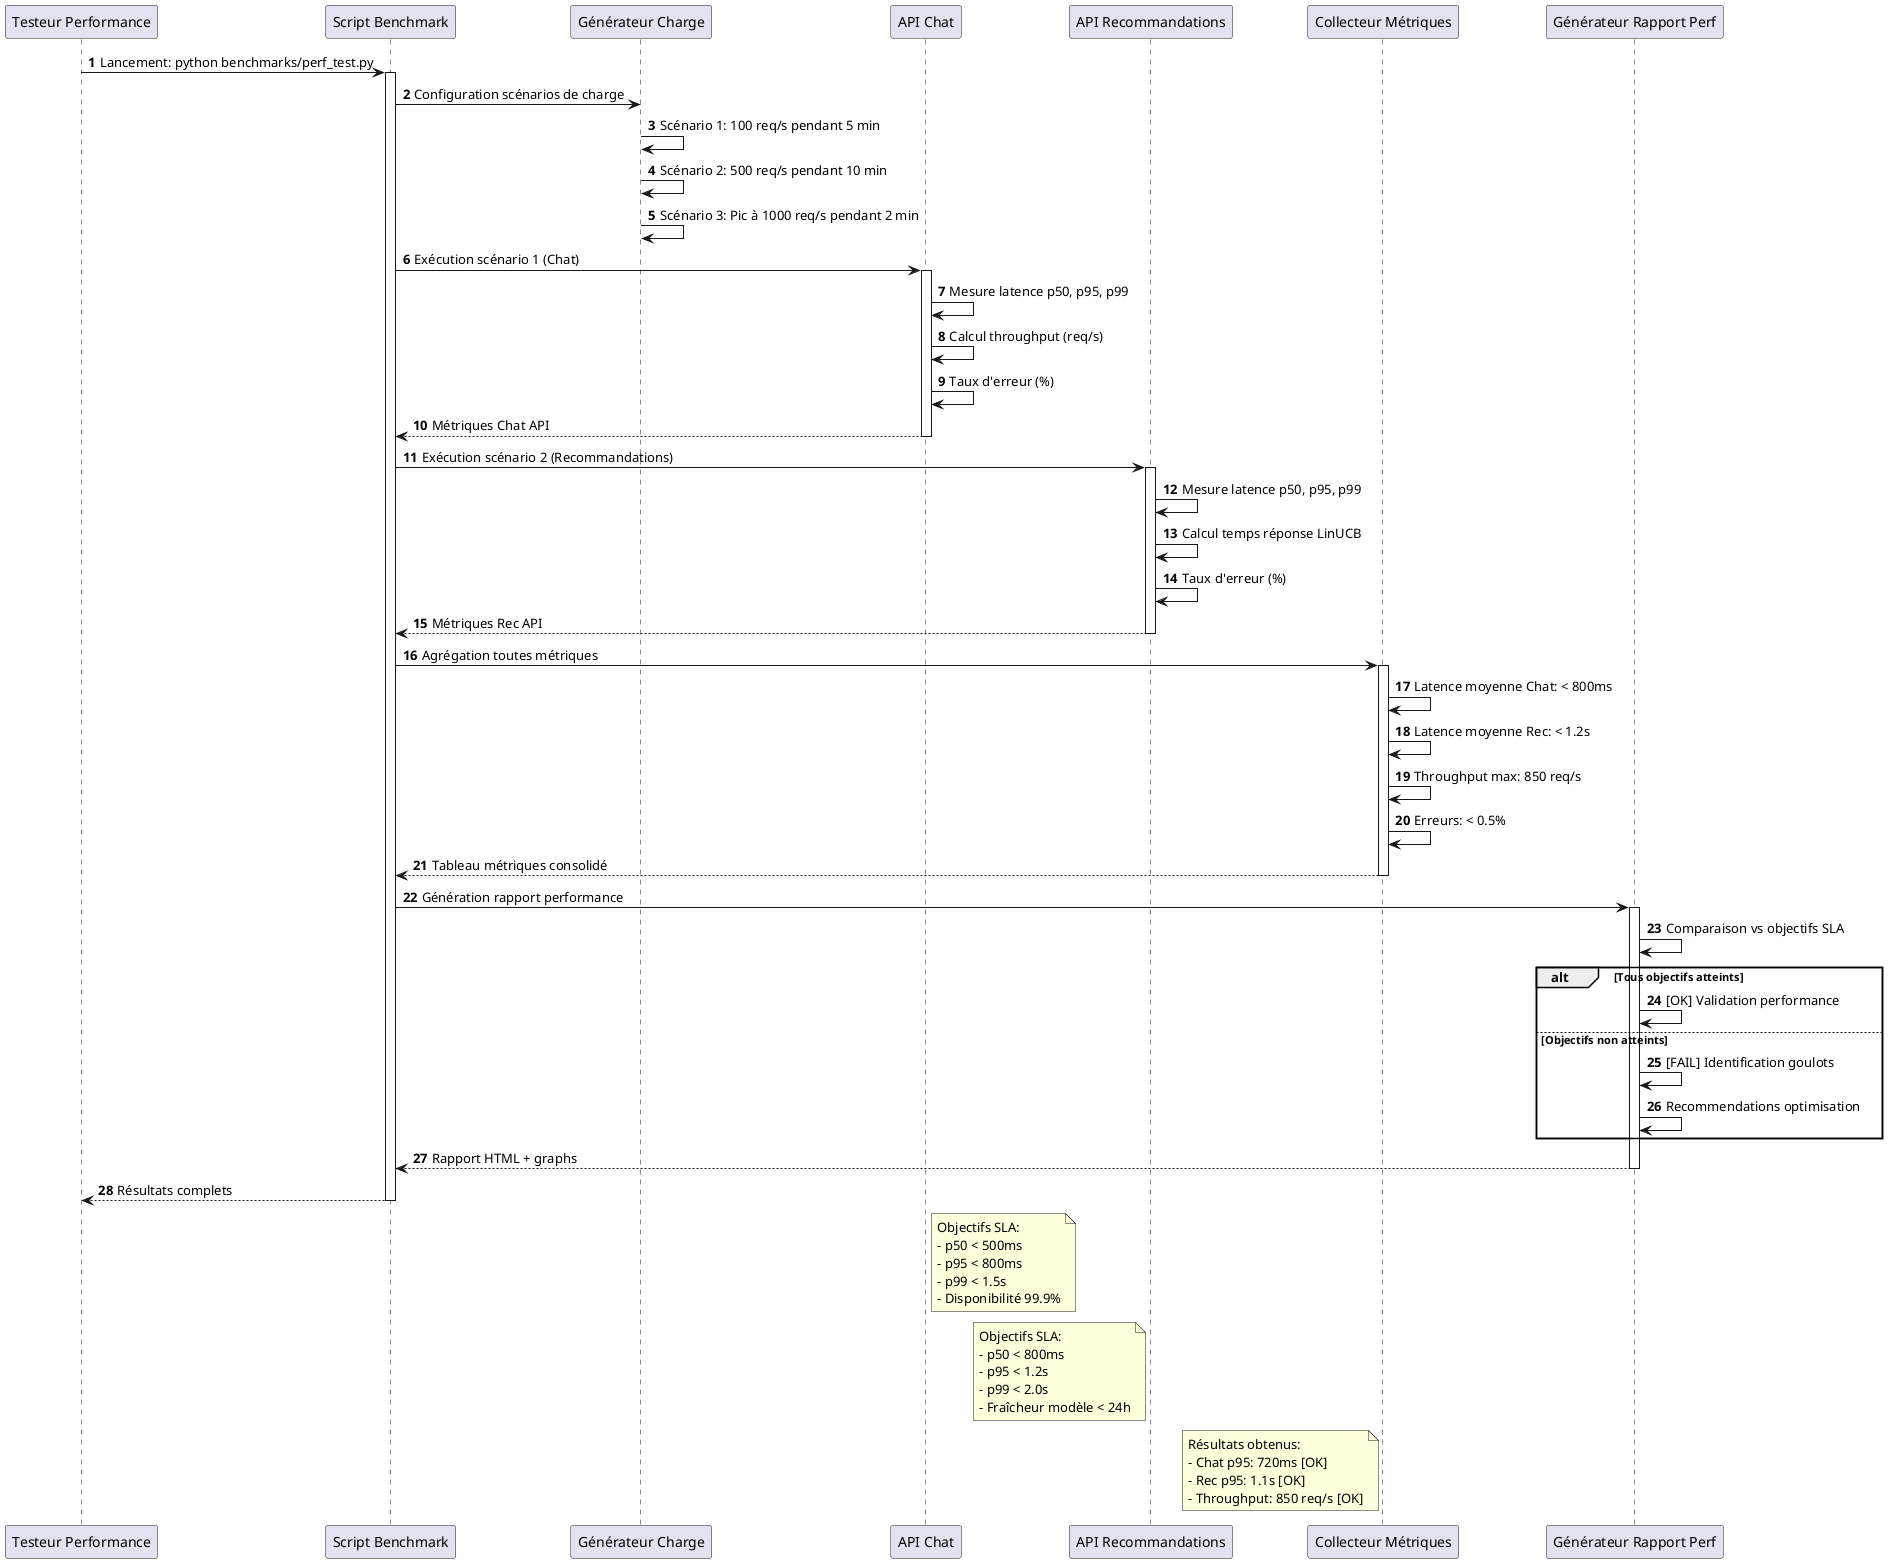
\includegraphics[width=\textwidth]{diagrams/plantuml/sequence_sprint3_secondary.png}
    \caption{Diagramme de séquence --- Modification d'un plan existant}
    \label{fig:seq_sprint3_secondary}
\end{figure}


% ────────────────────────────────────────────────────────────────
\section{Réalisation}
% ────────────────────────────────────────────────────────────────

\subsection{Machine à états LangGraph}

La machine à états de l'agent a été implémentée avec LangGraph. Le graphe articule quatre
nœuds principaux~: \textbf{THINK} interroge le LLM sélectionné, un routeur conditionnel
(\texttt{\_should\_continue()}) décide de la suite des opérations, \textbf{EXECUTE\_TOOL}
exécute l'outil appelé, \textbf{VALIDATE} vérifie la cohérence du plan, et \textbf{RESPOND}
formule la réponse finale. Après chaque exécution d'outil, le système reconduit l'agent vers
THINK pour réévaluation.

\begin{figure}[H]
    \centering
    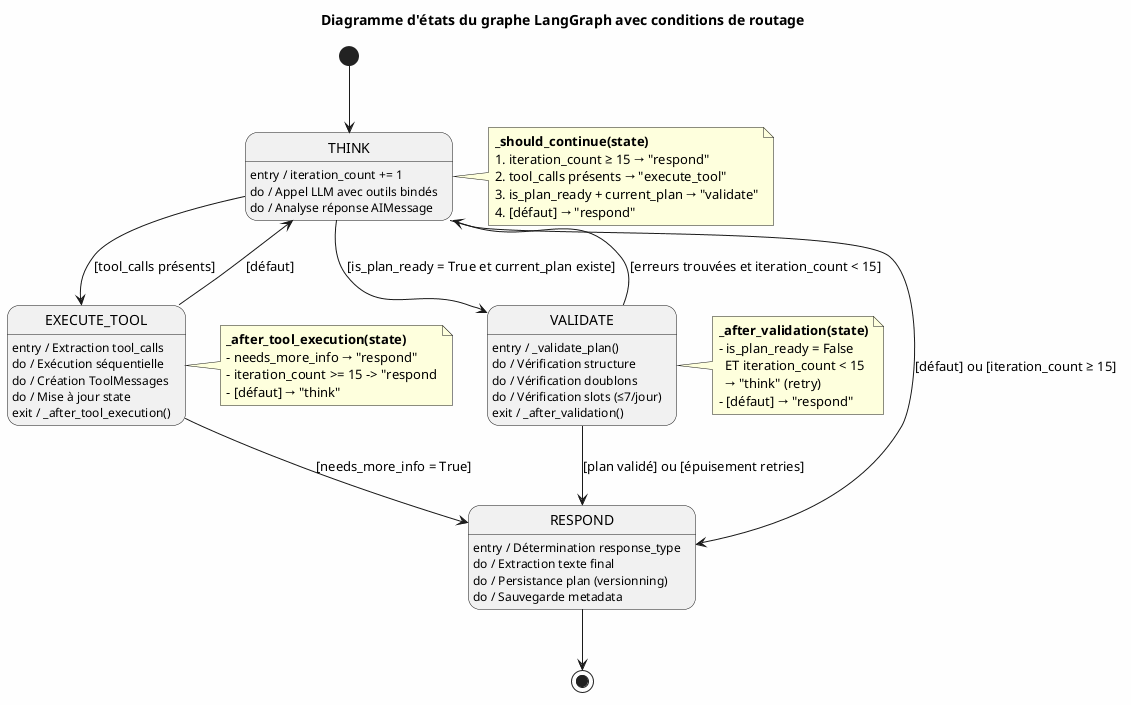
\includegraphics[width=0.75\textwidth]{diagrams/fig_04_langgraph_routing.png}
    \caption{Machine à états cyclique de l'agent planificateur}
    \label{fig:langgraph_graph}
\end{figure}

\subsection{Les 18 outils LLM-callable}

Un arsenal de dix-huit outils a été développé et enregistré dans un registre global~:

\begin{itemize}
    \item \textbf{Outils de recherche}~: \texttt{search\_activities}, \texttt{search\_stays},
    \texttt{search\_restaurants} pour la sélection géographique.
    \item \textbf{Outils contextuels}~: \texttt{get\_weather} (Open-Meteo),
    \texttt{get\_distance} (Haversine).
    \item \textbf{Outils RAG}~: \texttt{rag\_search}, \texttt{rag\_search\_for\_plan},
    \texttt{rag\_get\_similar} pour la recherche sémantique.
    \item \textbf{Outils de planification}~: \texttt{create\_plan\_structure},
    \texttt{modify\_plan}, \texttt{save\_plan\_tool} pour la construction du séjour.
    \item \textbf{Outil d'interaction}~: \texttt{ask\_user} pour questionner le touriste.
\end{itemize}

\subsection{Mémoire conversationnelle}

Le gestionnaire conversationnel emploie une politique de mémoire à taille glissante~: les
8~derniers messages sont systématiquement chargés. Lorsque la profondeur dépasse 15~messages,
un module résumeur contextuel extrait les points capitaux et se substitue aux messages anciens,
maintenant la cohérence sans surcharger le contexte du LLM.

\subsection{Abstraction multi-fournisseurs LLM}

Le patron fabrique (\textit{factory pattern}) implémenté dans \texttt{provider.py} permet
de basculer entre Ollama (local), Groq (rapide), Gemini (contexte long) et Lightning AI
via un simple paramètre de configuration, sans modification du code agentique.

\begin{table}[H]
    \centering
    \caption{Fournisseurs LLM intégrés dans Guidni}
    \label{tab:llm_providers}
    \small
    \begin{tabular}{p{2cm} p{3cm} p{1.5cm} p{2cm} p{4cm}}
        \toprule
        \textbf{Fournisseur} & \textbf{Modèle} & \textbf{Type} & \textbf{Latence} &
        \textbf{Caractéristique} \\
        \midrule
        Ollama & qwen2.5:7b & Local & 2--5\,s & Gratuit, hors-ligne \\[3pt]
        Groq & llama-3.3-70b & Cloud & 0.5--1\,s & Très rapide, 128k tokens \\[3pt]
        Gemini & gemini-2.5-flash & Cloud & 1--2\,s & Contexte 1M tokens \\[3pt]
        Lightning & openai/gpt-5 & Cloud & 1--3\,s & Dernière génération \\
        \bottomrule
    \end{tabular}
\end{table}

\subsection{Flux d'exécution des outils}

La figure suivante illustre le flux détaillé lorsqu'un outil est appelé par l'agent,
depuis la sélection par le LLM jusqu'au retour du résultat dans l'état.

\begin{figure}[H]
    \centering
    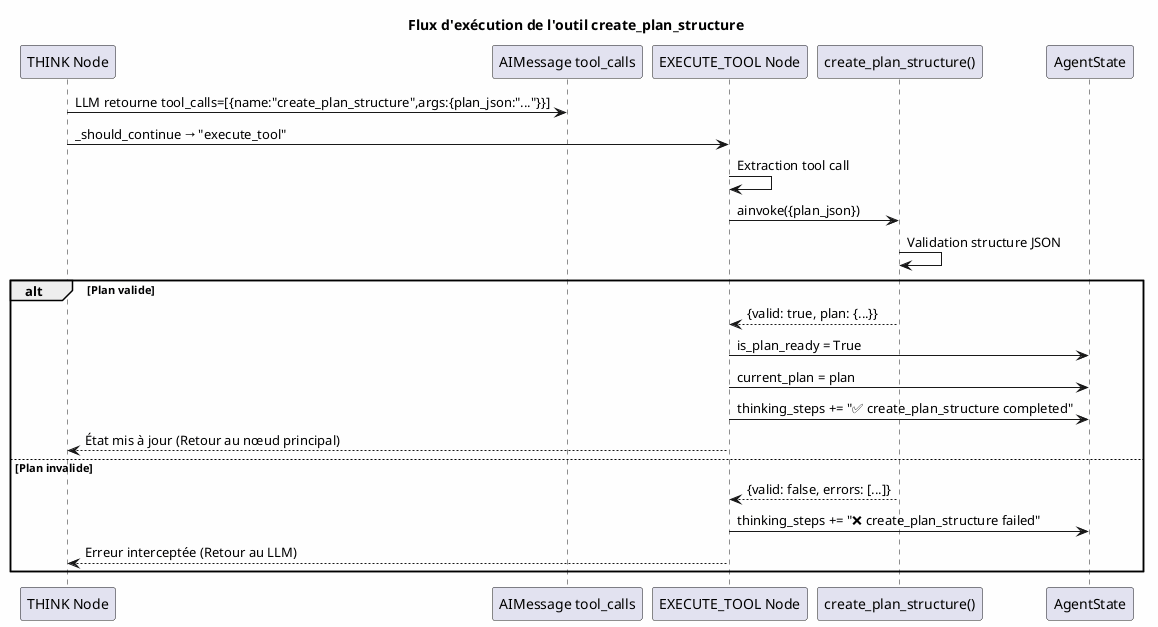
\includegraphics[width=0.85\textwidth]{diagrams/fig_04_tool_execution_flow.png}
    \caption{Flux d'exécution d'un outil par l'agent LangGraph}
    \label{fig:tool_exec_flow}
\end{figure}

\subsection{Démonstration de planification}

La figure suivante montre un exemple de conversation où l'agent génère un plan de 3~jours
à Djerba pour une famille, en orchestrant automatiquement les outils de recherche, météo
et planification.

\begin{figure}[H]
    \centering
    
\includegraphics[width=\textwidth]{diagrams/screen_04_chat_plan_output.png}
    \caption{Exemple de plan de voyage généré par l'agent}
    \label{fig:screen_plan}
\end{figure}

\begin{figure}[H]
    \centering
    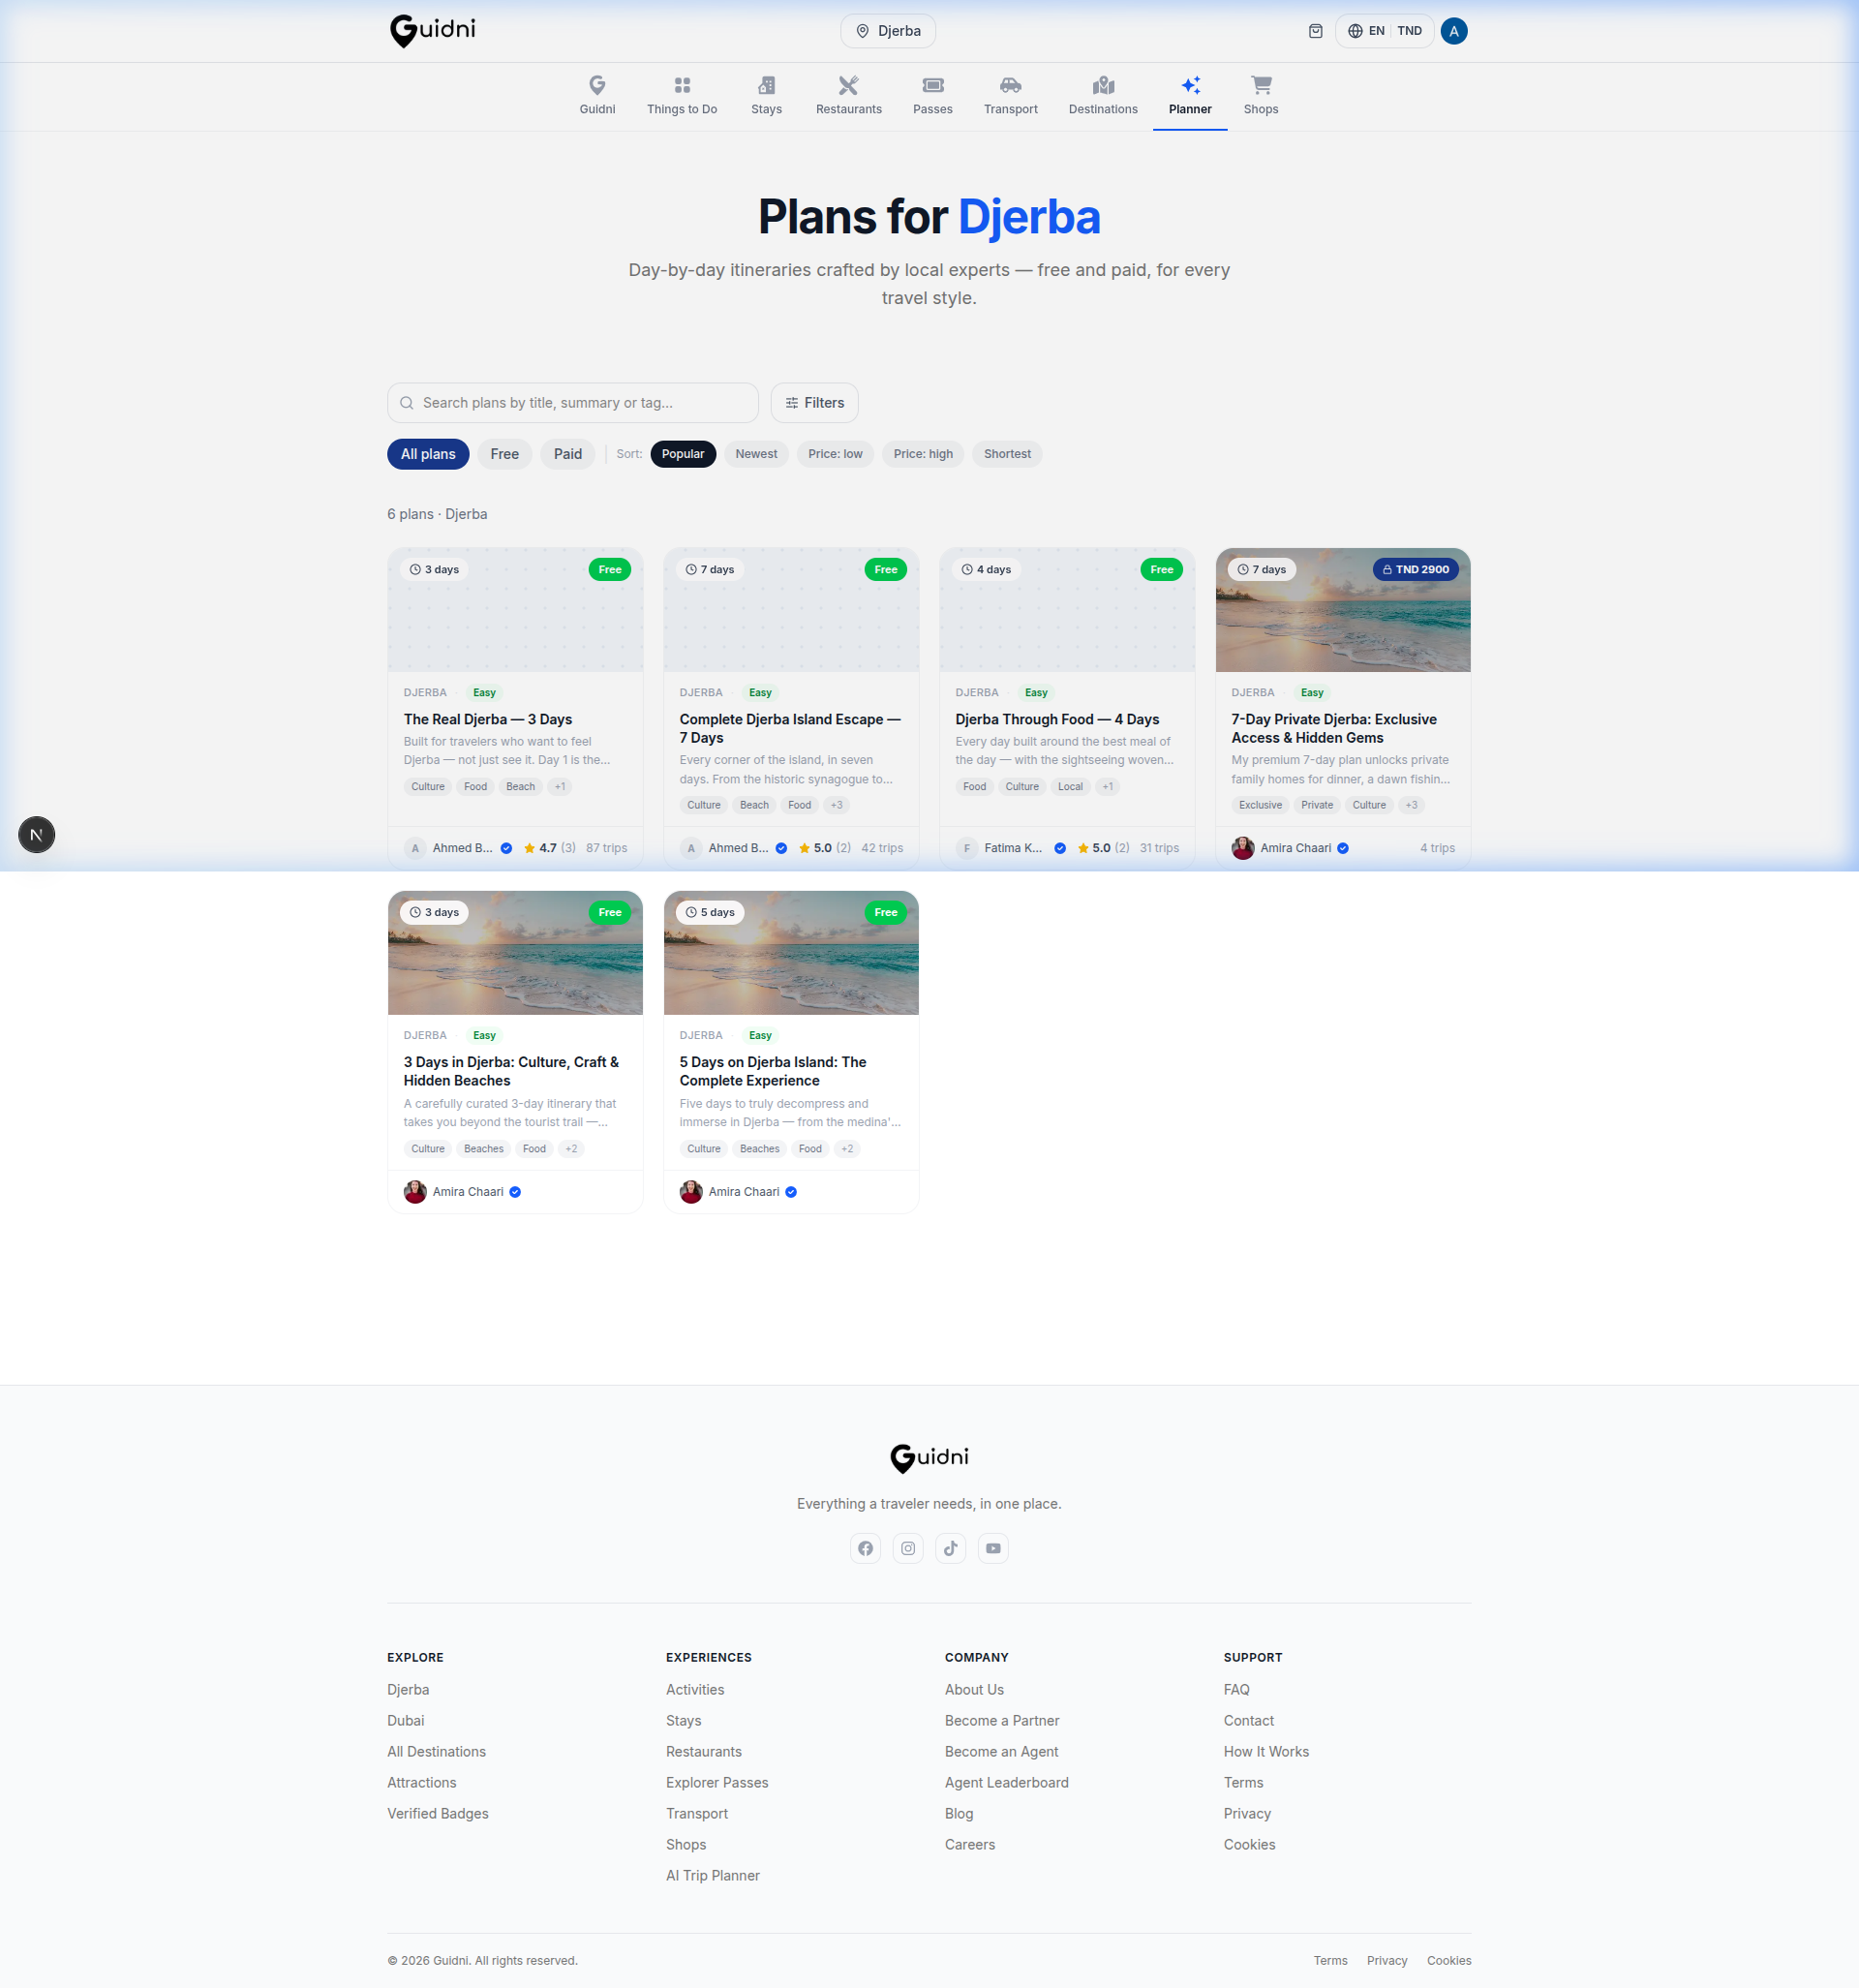
\includegraphics[width=\textwidth]{diagrams/screen_A4_plan_output_full.png}
    \caption{Plan de voyage complet affiché dans l'interface}
    \label{fig:screen_plan_full}
\end{figure}

\subsection{Étapes de raisonnement de l'agent}

La figure suivante montre les étapes de raisonnement (\textit{thinking steps}) visibles
dans les journaux du backend, attestant du cycle THINK $\rightarrow$ EXECUTE\_TOOL
$\rightarrow$ THINK successif avant la génération du plan final.

\begin{figure}[H]
    \centering
    
\includegraphics[width=\textwidth]{diagrams/screen_06_plan_thinking_steps.png}
    \caption{Étapes de raisonnement de l'agent planificateur}
    \label{fig:screen_thinking}
\end{figure}


% ────────────────────────────────────────────────────────────────
\section{Sprint Review}
% ────────────────────────────────────────────────────────────────

Lors de la Sprint Review, l'agent a fait la démonstration de sa robustesse en orchestrant une
dizaine d'appels d'outils successifs avant de produire un plan structuré validé. La
vérification des journaux détaillés a attesté le respect de la séquence cyclique du graphe et
des boucles de validation. L'encadrant a validé le Sprint.

Lors de la Sprint Retrospective, l'adoption de LangGraph a été jugée fructueuse pour la
transparence du raisonnement. L'équipe a identifié le besoin du moteur de recommandation
LinUCB pour gérer les interactions passives (navigation, défilement), justifiant le Sprint~4.


% ────────────────────────────────────────────────────────────────
\section*{Conclusion}
\addcontentsline{toc}{section}{Conclusion}

Le Sprint~3 a permis de construire le cœur intelligent de Guidni~: l'agent planificateur
LangGraph avec ses quatre nœuds, ses dix-huit outils et son système de mémoire
conversationnelle. L'abstraction multi-fournisseurs LLM offre une flexibilité de déploiement.
Le Sprint~4 sera consacré à l'implémentation du moteur de recommandation LinUCB, aux tests
d'évaluation et à la finalisation du système.


\chapter{Sprint~4~: Moteur LinUCB, Tests et Évaluation}
% ============================================================================
% CHAPITRE 6 — SPRINT 4 : MOTEUR LinUCB, TESTS ET ÉVALUATION
% ============================================================================

\section{Introduction}

Ce chapitre détaille le déroulement du Sprint~4, dernier Sprint du projet Guidni. Ce
quatrième Sprint, d'une durée de six semaines (janvier--février 2025), est consacré à
l'implémentation du moteur de recommandation LinUCB, aux tests et à l'évaluation globale
du système. Pour cela, j'ai suivi le plan suivant~:
\begin{enumerate}
    \item Planning du Sprint
    \item Analyse
    \item Conception
    \item Réalisation
    \item Sprint Review
\end{enumerate}


% ────────────────────────────────────────────────────────────────
\section{Planning du Sprint~4}
% ────────────────────────────────────────────────────────────────

\subsection{Objectif du Sprint}

L'objectif du Sprint~4 est double~: d'une part, implémenter le moteur de recommandation
Hybride LinUCB capable de scorer les recommandations en moins de 100~ms grâce au cache
matriciel en RAM~; d'autre part, mener les campagnes de tests et d'évaluation quantitative
pour valider l'ensemble du système Guidni.

\subsection{Sprint Backlog}

\begin{table}[H]
    \centering
    \caption{Sprint Backlog --- Sprint~4}
    \label{tab:sprint4_backlog}
    \small
    \begin{tabular}{c c p{6.5cm} c}
        \toprule
        \textbf{ID US} & \textbf{ID Task} & \textbf{Task} & \textbf{Complexité} \\
        \midrule
        US-06 & T-4.1 & Implémentation du moteur de scoring LinUCB & XL \\[3pt]
        US-06 & T-4.2 & Implémentation de l'ingénierie des caractéristiques ($\phi$) & L \\[3pt]
        US-06 & T-4.3 & Pipeline de classement post-LinUCB en 10 étapes & XL \\[3pt]
        US-07 & T-4.4 & Cache matriciel en RAM avec verrou threading & L \\[3pt]
        US-08 & T-4.5 & Implémentation du tracker JavaScript vanilla & L \\[3pt]
        US-08 & T-4.6 & Endpoint \texttt{POST /api/recommendations/events} & M \\[3pt]
        US-11 & T-4.7 & Jobs nocturnes APScheduler (profils, dérive, tags) & M \\[3pt]
        US-12 & T-4.8 & Vérification d'intégrité vocabulaire par SHA-256 & S \\[3pt]
        US-06 & T-4.9 & Tests unitaires et d'intégration (pytest) & L \\[3pt]
        US-04 & T-4.10 & Évaluation du pipeline RAG (20 requêtes test) & M \\[3pt]
        US-06 & T-4.11 & Simulation du moteur LinUCB (500 sessions) & L \\
        \bottomrule
    \end{tabular}
\end{table}

\subsection{Definition of Done (DoD)}

\begin{itemize}
    \item La recommandation s'effectue et s'affiche sous un seuil de latence de 100~ms.
    \item L'adaptation du scoring est démontrée en fonction des récompenses accumulées.
    \item Les tests unitaires et d'intégration passent sans échec.
    \item L'évaluation RAG sur 20~requêtes multilingues confirme la pertinence sémantique.
    \item La simulation LinUCB sur 500~sessions démontre la convergence prédictive.
\end{itemize}


% ────────────────────────────────────────────────────────────────
\section{Analyse}
% ────────────────────────────────────────────────────────────────

\subsection{Diagramme de cas d'utilisation}

\begin{figure}[H]
    \centering
    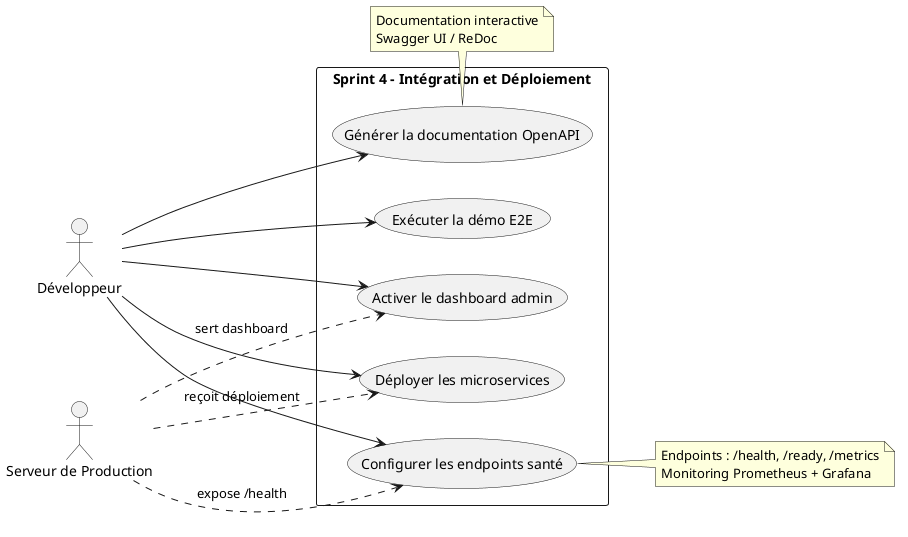
\includegraphics[width=0.85\textwidth]{diagrams/plantuml/usecase_sprint4.png}
    \caption{Diagramme de cas d'utilisation --- Sprint~4}
    \label{fig:uc_sprint4}
\end{figure}

\subsection{Description textuelle des cas d'utilisation}

\begin{table}[H]
    \centering
    \caption{Description textuelle --- CU : Obtenir des recommandations personnalisées}
    \label{tab:cu_sprint4_1}
    \small
    \begin{tabular}{p{3cm} p{10cm}}
        \toprule
        \textbf{Champ} & \textbf{Description} \\
        \midrule
        Titre & Obtenir des recommandations personnalisées \\[3pt]
        Acteur & Touriste / Système \\[3pt]
        Pré-condition & Des bras \texttt{BanditArm} existent pour la zone demandée \\[3pt]
        Scénario nominal &
        1. Le frontend envoie \texttt{GET /api/recommendations} avec paramètres de contexte \newline
        2. Les bras sont récupérés depuis le cache RAM \newline
        3. Le profil utilisateur est chargé si \texttt{user\_id} est fourni \newline
        4. Le vecteur $\phi$ est calculé par produit de Kronecker pour chaque bras \newline
        5. Le pipeline de classement en 10~étapes est exécuté \newline
        6. Les Top-K recommandations sont retournées \\[3pt]
        Post-condition & Un \texttt{RecommendationEvent} de type impression est enregistré \\
        \bottomrule
    \end{tabular}
\end{table}

\begin{table}[H]
    \centering
    \caption{Description textuelle --- CU : Tracker un événement comportemental}
    \label{tab:cu_sprint4_2}
    \small
    \begin{tabular}{p{3cm} p{10cm}}
        \toprule
        \textbf{Champ} & \textbf{Description} \\
        \midrule
        Titre & Tracker un événement comportemental \\[3pt]
        Acteur & Système (tracker JavaScript) \\[3pt]
        Pré-condition & Session active avec un \texttt{session\_id} valide \\[3pt]
        Scénario nominal &
        1. Le tracker JS détecte un événement (clic, scroll, favoris, réservation) \newline
        2. L'événement est mis en file d'attente \newline
        3. Flush toutes les 15~secondes ou tous les 10~événements \newline
        4. \texttt{POST /api/recommendations/events} envoie le lot \newline
        5. \texttt{compute\_reward()} calcule la récompense delta \newline
        6. Les matrices A et b sont mises à jour en RAM \\[3pt]
        Post-condition & Compteurs \texttt{BanditArm} et \texttt{RecommendationEvent} mis à jour \\
        \bottomrule
    \end{tabular}
\end{table}


% ────────────────────────────────────────────────────────────────
\section{Conception}
% ────────────────────────────────────────────────────────────────

\subsection{Diagramme de séquence --- Pipeline de recommandation}

\begin{figure}[H]
    \centering
    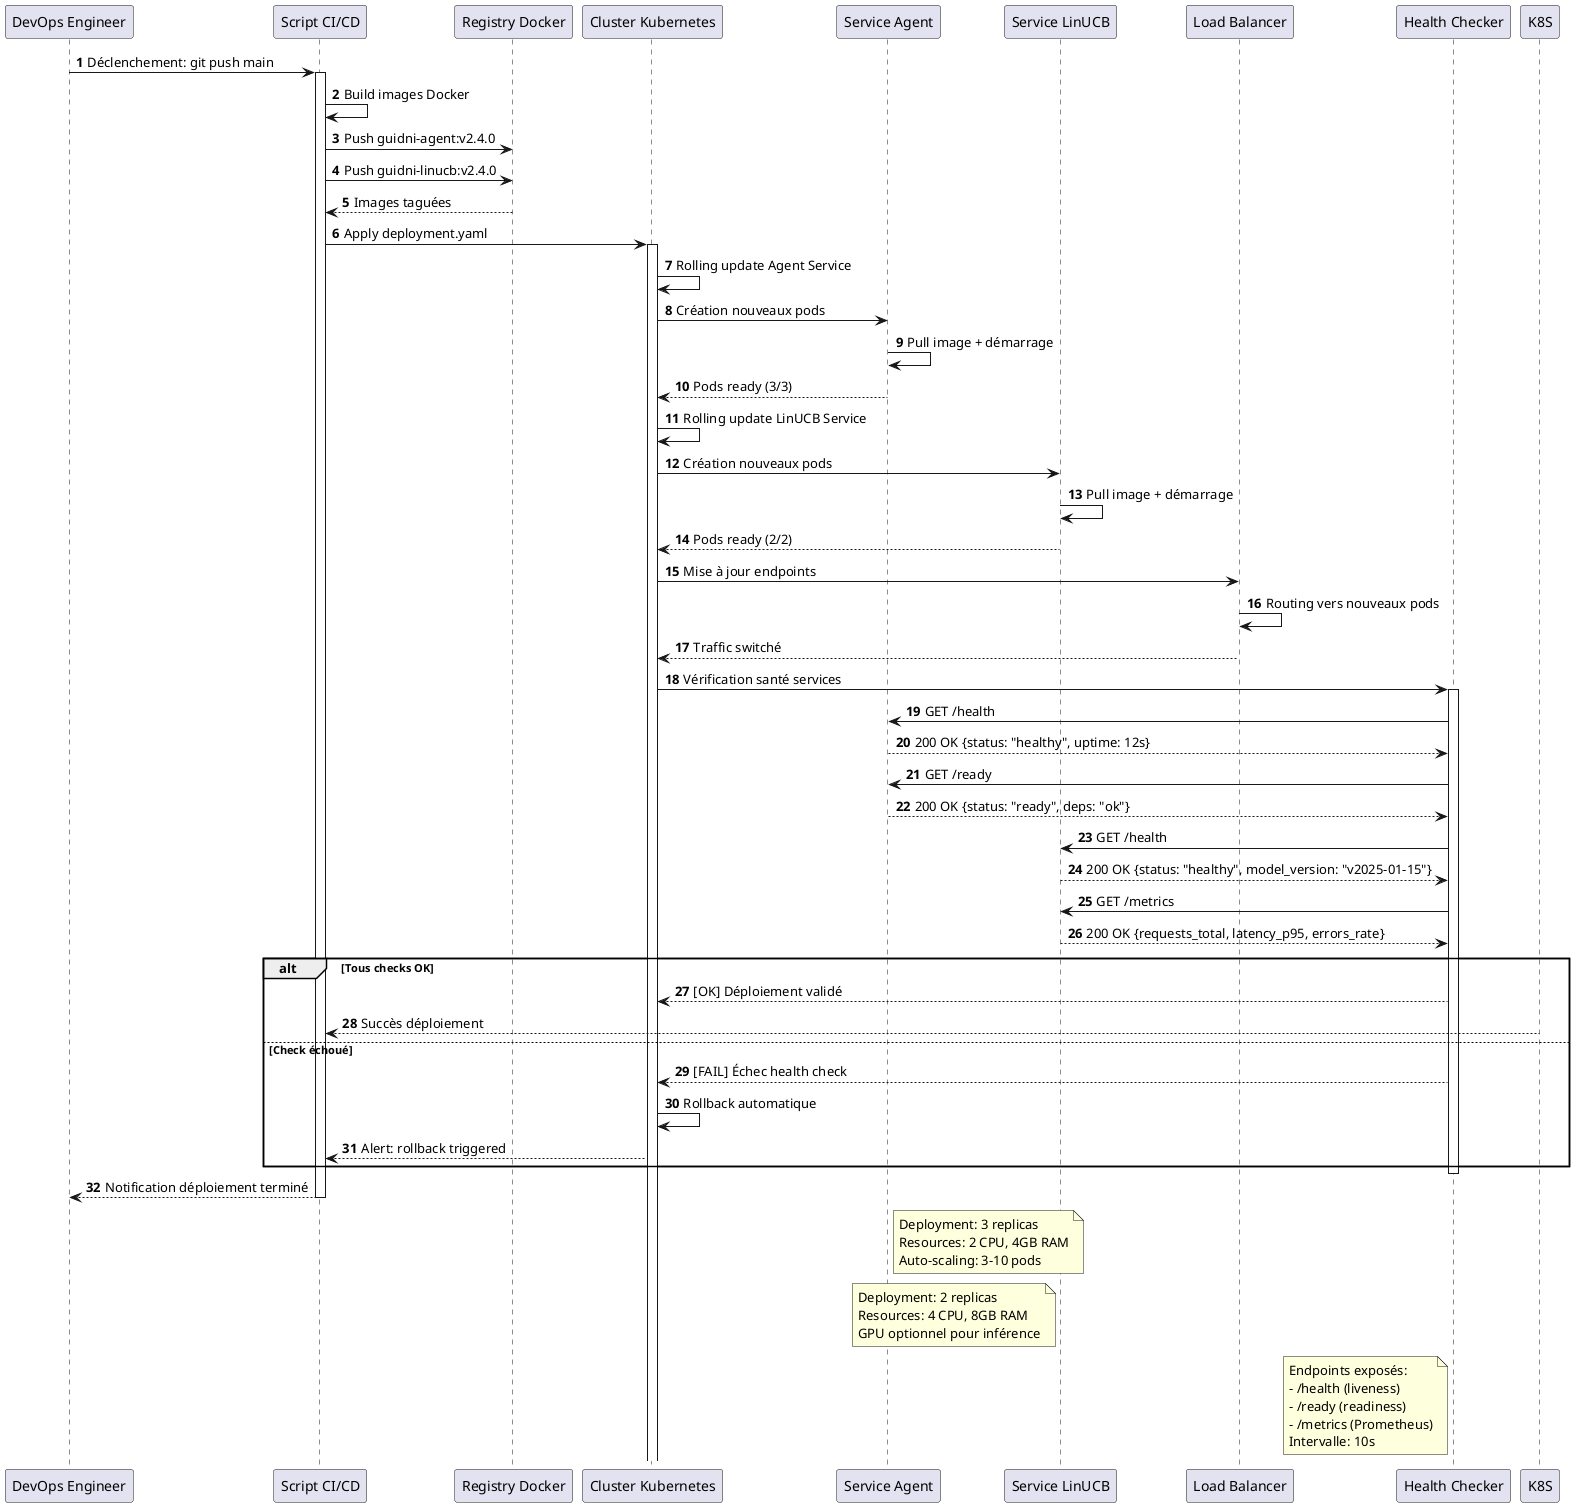
\includegraphics[width=\textwidth]{diagrams/plantuml/sequence_sprint4_primary.png}
    \caption{Diagramme de séquence --- Pipeline de recommandation LinUCB}
    \label{fig:seq_sprint4_primary}
\end{figure}

\subsection{Diagramme de séquence --- Traitement des événements comportementaux}

\begin{figure}[H]
    \centering
    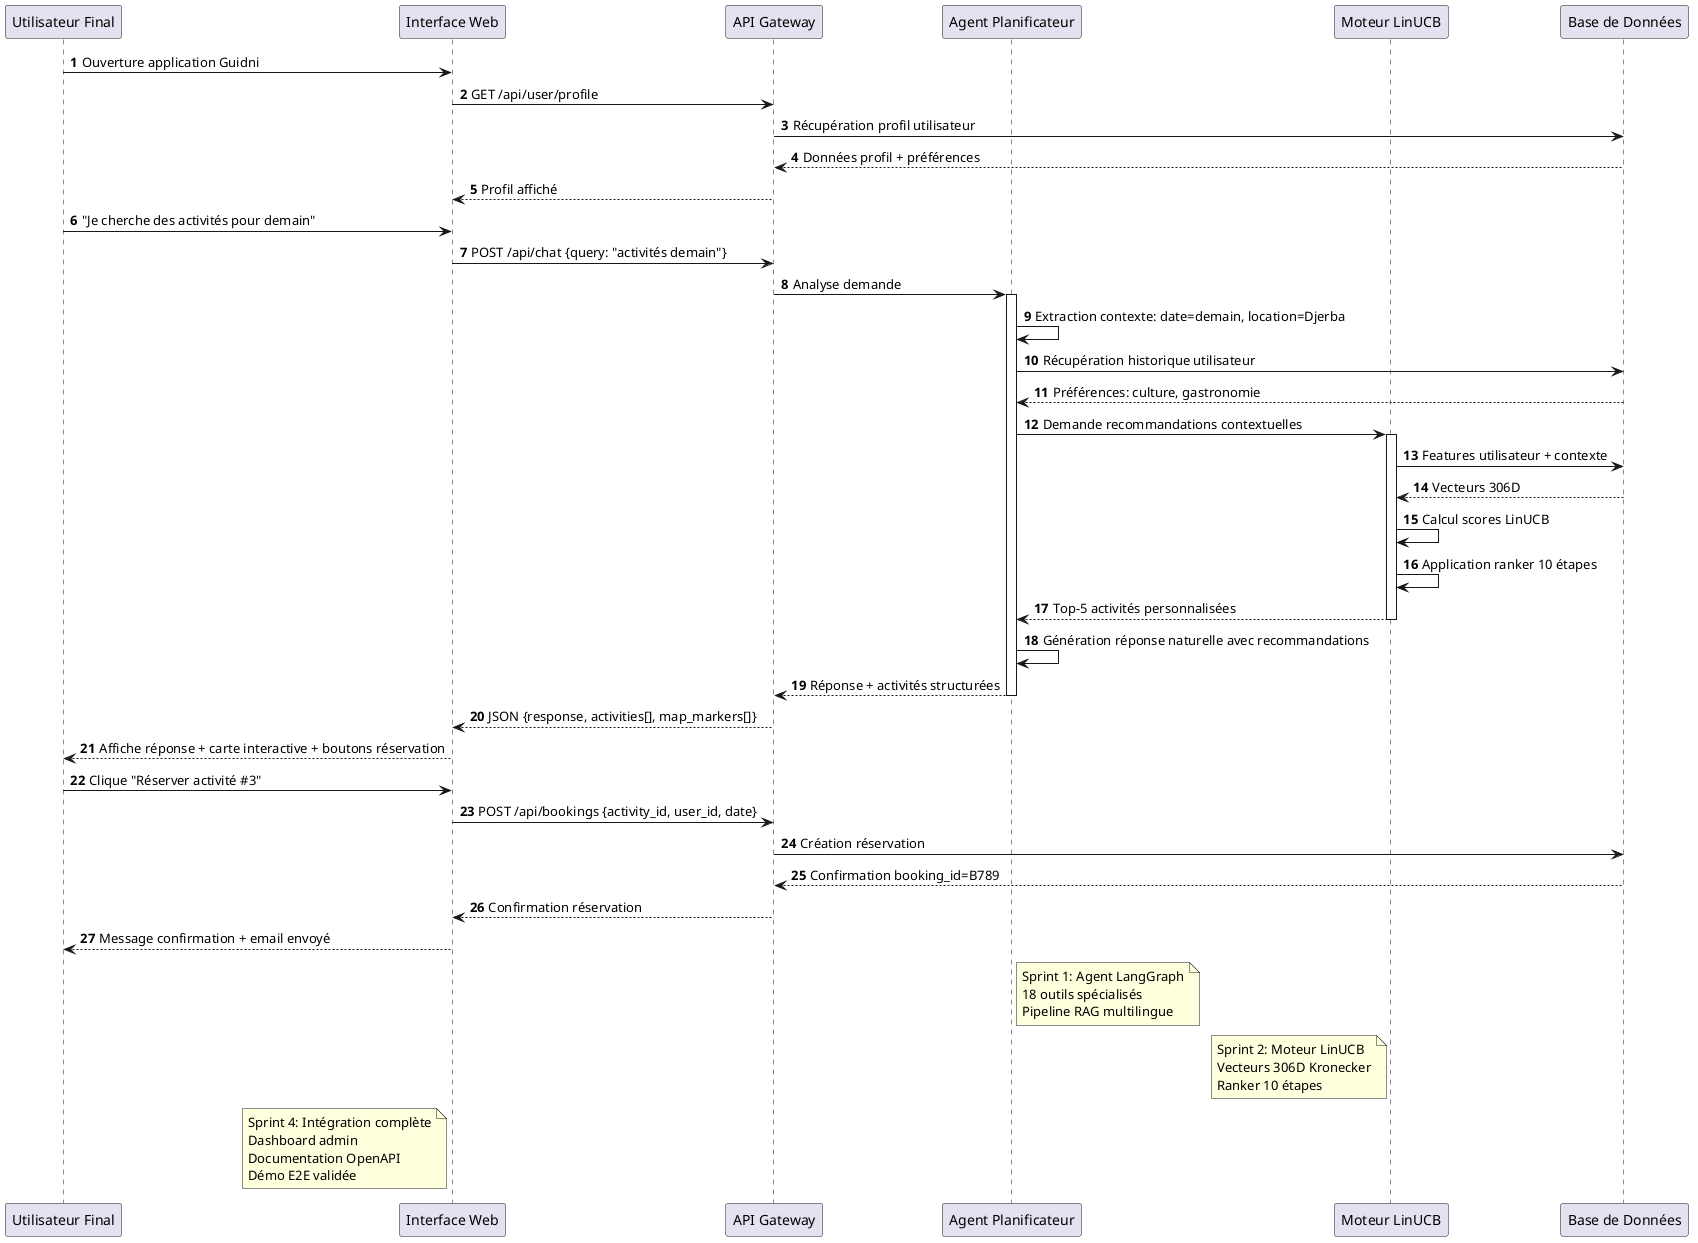
\includegraphics[width=\textwidth]{diagrams/plantuml/sequence_sprint4_secondary.png}
    \caption{Diagramme de séquence --- Traitement d'un lot d'événements comportementaux}
    \label{fig:seq_sprint4_secondary}
\end{figure}


% ────────────────────────────────────────────────────────────────
\section{Réalisation}
% ────────────────────────────────────────────────────────────────

\subsection{Processus du moteur LinUCB}

La figure suivante illustre le cycle d'exploitation/exploration du moteur LinUCB, depuis
la réception du contexte utilisateur jusqu'à la mise à jour des matrices suite à la
récompense observée.

\begin{figure}[H]
    \centering
    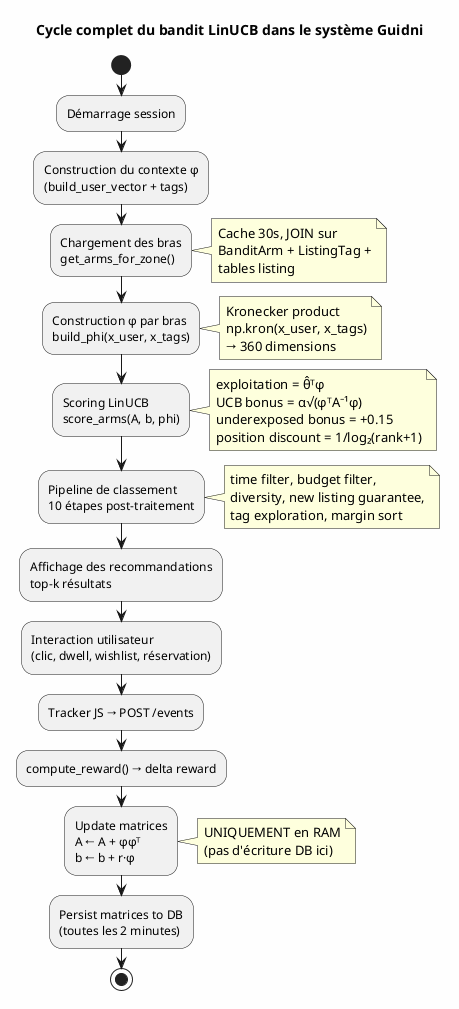
\includegraphics[width=0.75\textwidth]{diagrams/fig_02_linucb_cycle.png}
    \caption{Processus du moteur LinUCB --- cycle exploitation/exploration}
    \label{fig:linucb_process}
\end{figure}

\subsection{Moteur de scoring LinUCB}

Le moteur LinUCB a été implémenté avec les composants suivants~:

\begin{itemize}
    \item \textbf{Vecteur de caractéristiques} $\phi$ de dimension~306, construit par produit
    de Kronecker~: $\phi = x_{\text{user}}(9) \otimes x_{\text{tags}}(34)$.
    \item \textbf{Matrice globale} $A$ ($306 \times 306$) et vecteur cible $b$ ($306$),
    partagés entre toutes les annonces dans \texttt{LinUCBGlobal}.
    \item \textbf{Cache en RAM} avec verrou \texttt{threading.Lock} pour un accès quasi
    instantané, avec persistance asynchrone en base toutes les 2~minutes via APScheduler.
    \item \textbf{Score UCB}~: $\text{score} = \hat{\theta}^\top \phi + \alpha
    \sqrt{\phi^\top A^{-1} \phi}$ avec $\alpha = 0.3$.
\end{itemize}

\begin{table}[H]
    \centering
    \caption{Les 9 composantes du vecteur utilisateur $x_{\text{user}}$}
    \label{tab:user_vector}
    \small
    \begin{tabular}{c l l}
        \toprule
        \textbf{Idx} & \textbf{Caractéristique} & \textbf{Formule} \\
        \midrule
        0 & sin(heure) & $\sin(2\pi \times h / 24)$ \\
        1 & cos(heure) & $\cos(2\pi \times h / 24)$ \\
        2 & sin(mois) & $\sin(2\pi \times m / 12)$ \\
        3 & cos(mois) & $\cos(2\pi \times m / 12)$ \\
        4 & Profondeur défilement & $\text{clip}(\text{scroll}, 0, 1)$ \\
        5 & Temps consultation & $\text{clip}(\log(1+\text{dwell})/\log(301), 0, 1)$ \\
        6 & Affinité prix & $\text{avg\_price} / 2000$ \\
        7 & Affinité tag max & $\max(\text{tag\_affinity})$ \\
        8 & Type voyage & famille$=1.0$, couple$=0.67$, solo$=0.33$ \\
        \bottomrule
    \end{tabular}
\end{table}

\subsection{Pipeline de classement en 10 étapes}

Le fichier \texttt{ranker.py} déploie un pipeline séquentiel en dix étapes~:
\begin{enumerate}
    \item Correction de popularité (bonus +0.15 si $<$50 impressions)
    \item Filtre temporel (pas de bar le matin, pas d'activité matinale le soir)
    \item Filtre budgétaire (prix $\leq$ budget $\times$ 1.25)
    \item Construction des vecteurs $\phi$ (produit de Kronecker)
    \item Scoring LinUCB (formule UCB)
    \item Filtre de diversité (max 2 annonces par type)
    \item Garantie nouvelles annonces (1 sous-exposée minimum)
    \item Exploration de tags (10\% de tags non explorés)
    \item Tri par marge (commission pour les ex-æquo)
    \item Extraction Top-K (10 par défaut)
\end{enumerate}

\begin{figure}[H]
    \centering
    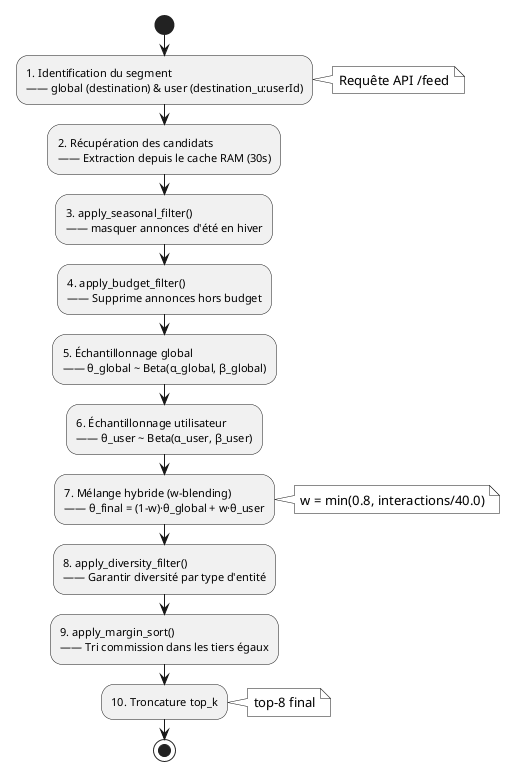
\includegraphics[width=0.85\textwidth]{diagrams/fig_05_ranker_pipeline.png}
    \caption{Organigramme du pipeline de classement en 10 étapes}
    \label{fig:ranker_pipeline}
\end{figure}

\subsection{Tracker comportemental JavaScript}

Le tracker JavaScript vanilla, sans dépendance externe, analyse le navigateur du client et
collecte huit types de signaux avec des valeurs de récompense prédéfinies~:

\begin{table}[H]
    \centering
    \caption{Signaux de récompense du tracker comportemental}
    \label{tab:rewards}
    \small
    \begin{tabular}{l c l}
        \toprule
        \textbf{Signal} & \textbf{Récompense} & \textbf{Description} \\
        \midrule
        quick\_exit & $-0.2$ & Sortie en $<$5 secondes \\
        impression & $0.0$ & Simple affichage \\
        click & $0.3$ & Clic sur l'annonce \\
        gallery\_swipe & $0.4$ & Balayage de la galerie \\
        dwell\_30s & $0.5$ & Consultation $\geq$30 secondes \\
        scroll\_reviews & $0.6$ & Lecture des avis \\
        dwell\_60s & $0.7$ & Consultation $\geq$60 secondes \\
        wishlist & $0.85$ & Ajout aux favoris \\
        reservation & $1.0$ & Réservation ferme \\
        \bottomrule
    \end{tabular}
\end{table}

\begin{figure}[H]
    \centering
    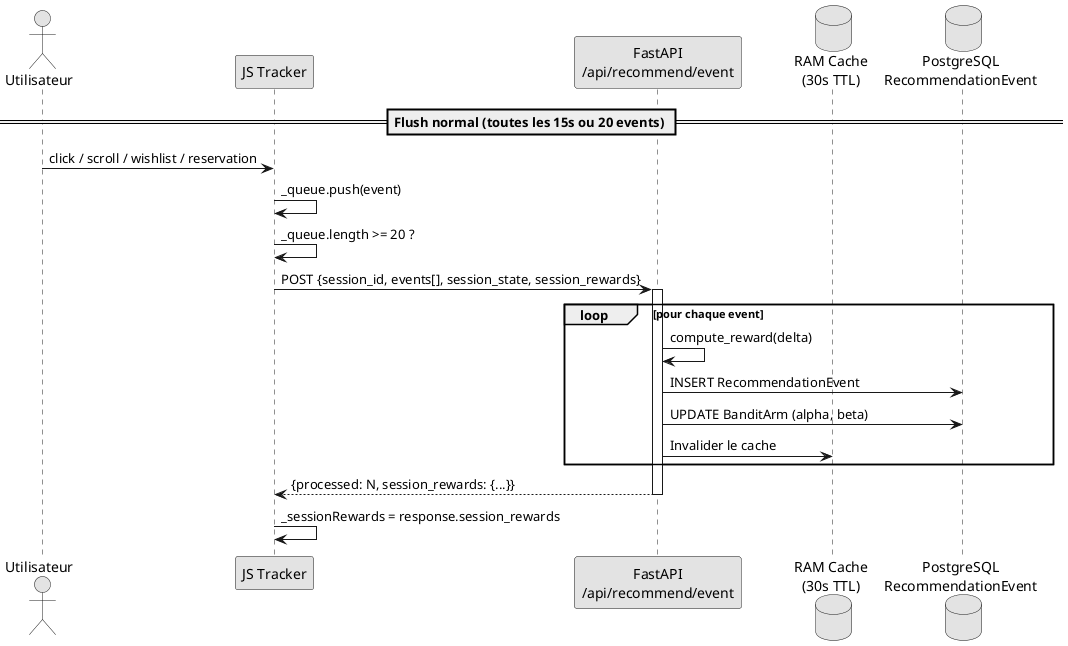
\includegraphics[width=0.85\textwidth]{diagrams/fig_05_tracker_flush.png}
    \caption{Flux du tracker JavaScript --- mise en file d'attente et flush par lot}
    \label{fig:tracker_flush}
\end{figure}

\subsection{Stratégie de tests}

La stratégie de tests stratifiée, orchestrée par \texttt{pytest}, comprend trois couches~:
\begin{itemize}
    \item \textbf{Tests unitaires}~: chaque fonction pure (normalisation des vecteurs $\phi$,
    filtrage budgétaire, calcul de score) testée par assertion.
    \item \textbf{Tests d'intégration}~: fluidité des interactions entre composants et
    persistance relationnelle (Event Loop FastAPI sans blocage).
    \item \textbf{Tests système}~: orchestration end-to-end de l'agent LangGraph avec les
    18~outils.
\end{itemize}

\subsection{Évaluation du pipeline RAG}

L'évaluation quantitative repose sur l'injection de 20~requêtes test couvrant le spectre
trilingue (FR/EN/AR) avec des critères discriminants~: contraintes géographiques, notions
subjectives (romantisme, adrénaline) et limitations budgétaires. Les résultats attestent
d'une préservation sémantique élevée (Precision@K) justifiant l'hybridation multilingue.

\subsection{Simulation du moteur LinUCB}

Un banc d'essai émulant 500~sessions d'exploration avec des comportements de clics orientés
a été programmé. Le cumul de la récompense (Cumulative Reward) croît significativement au fil
des itérations, supplantant une stratégie aléatoire et démontrant le franchissement de la
phase de Cold Start.

\begin{figure}[H]
    \centering
    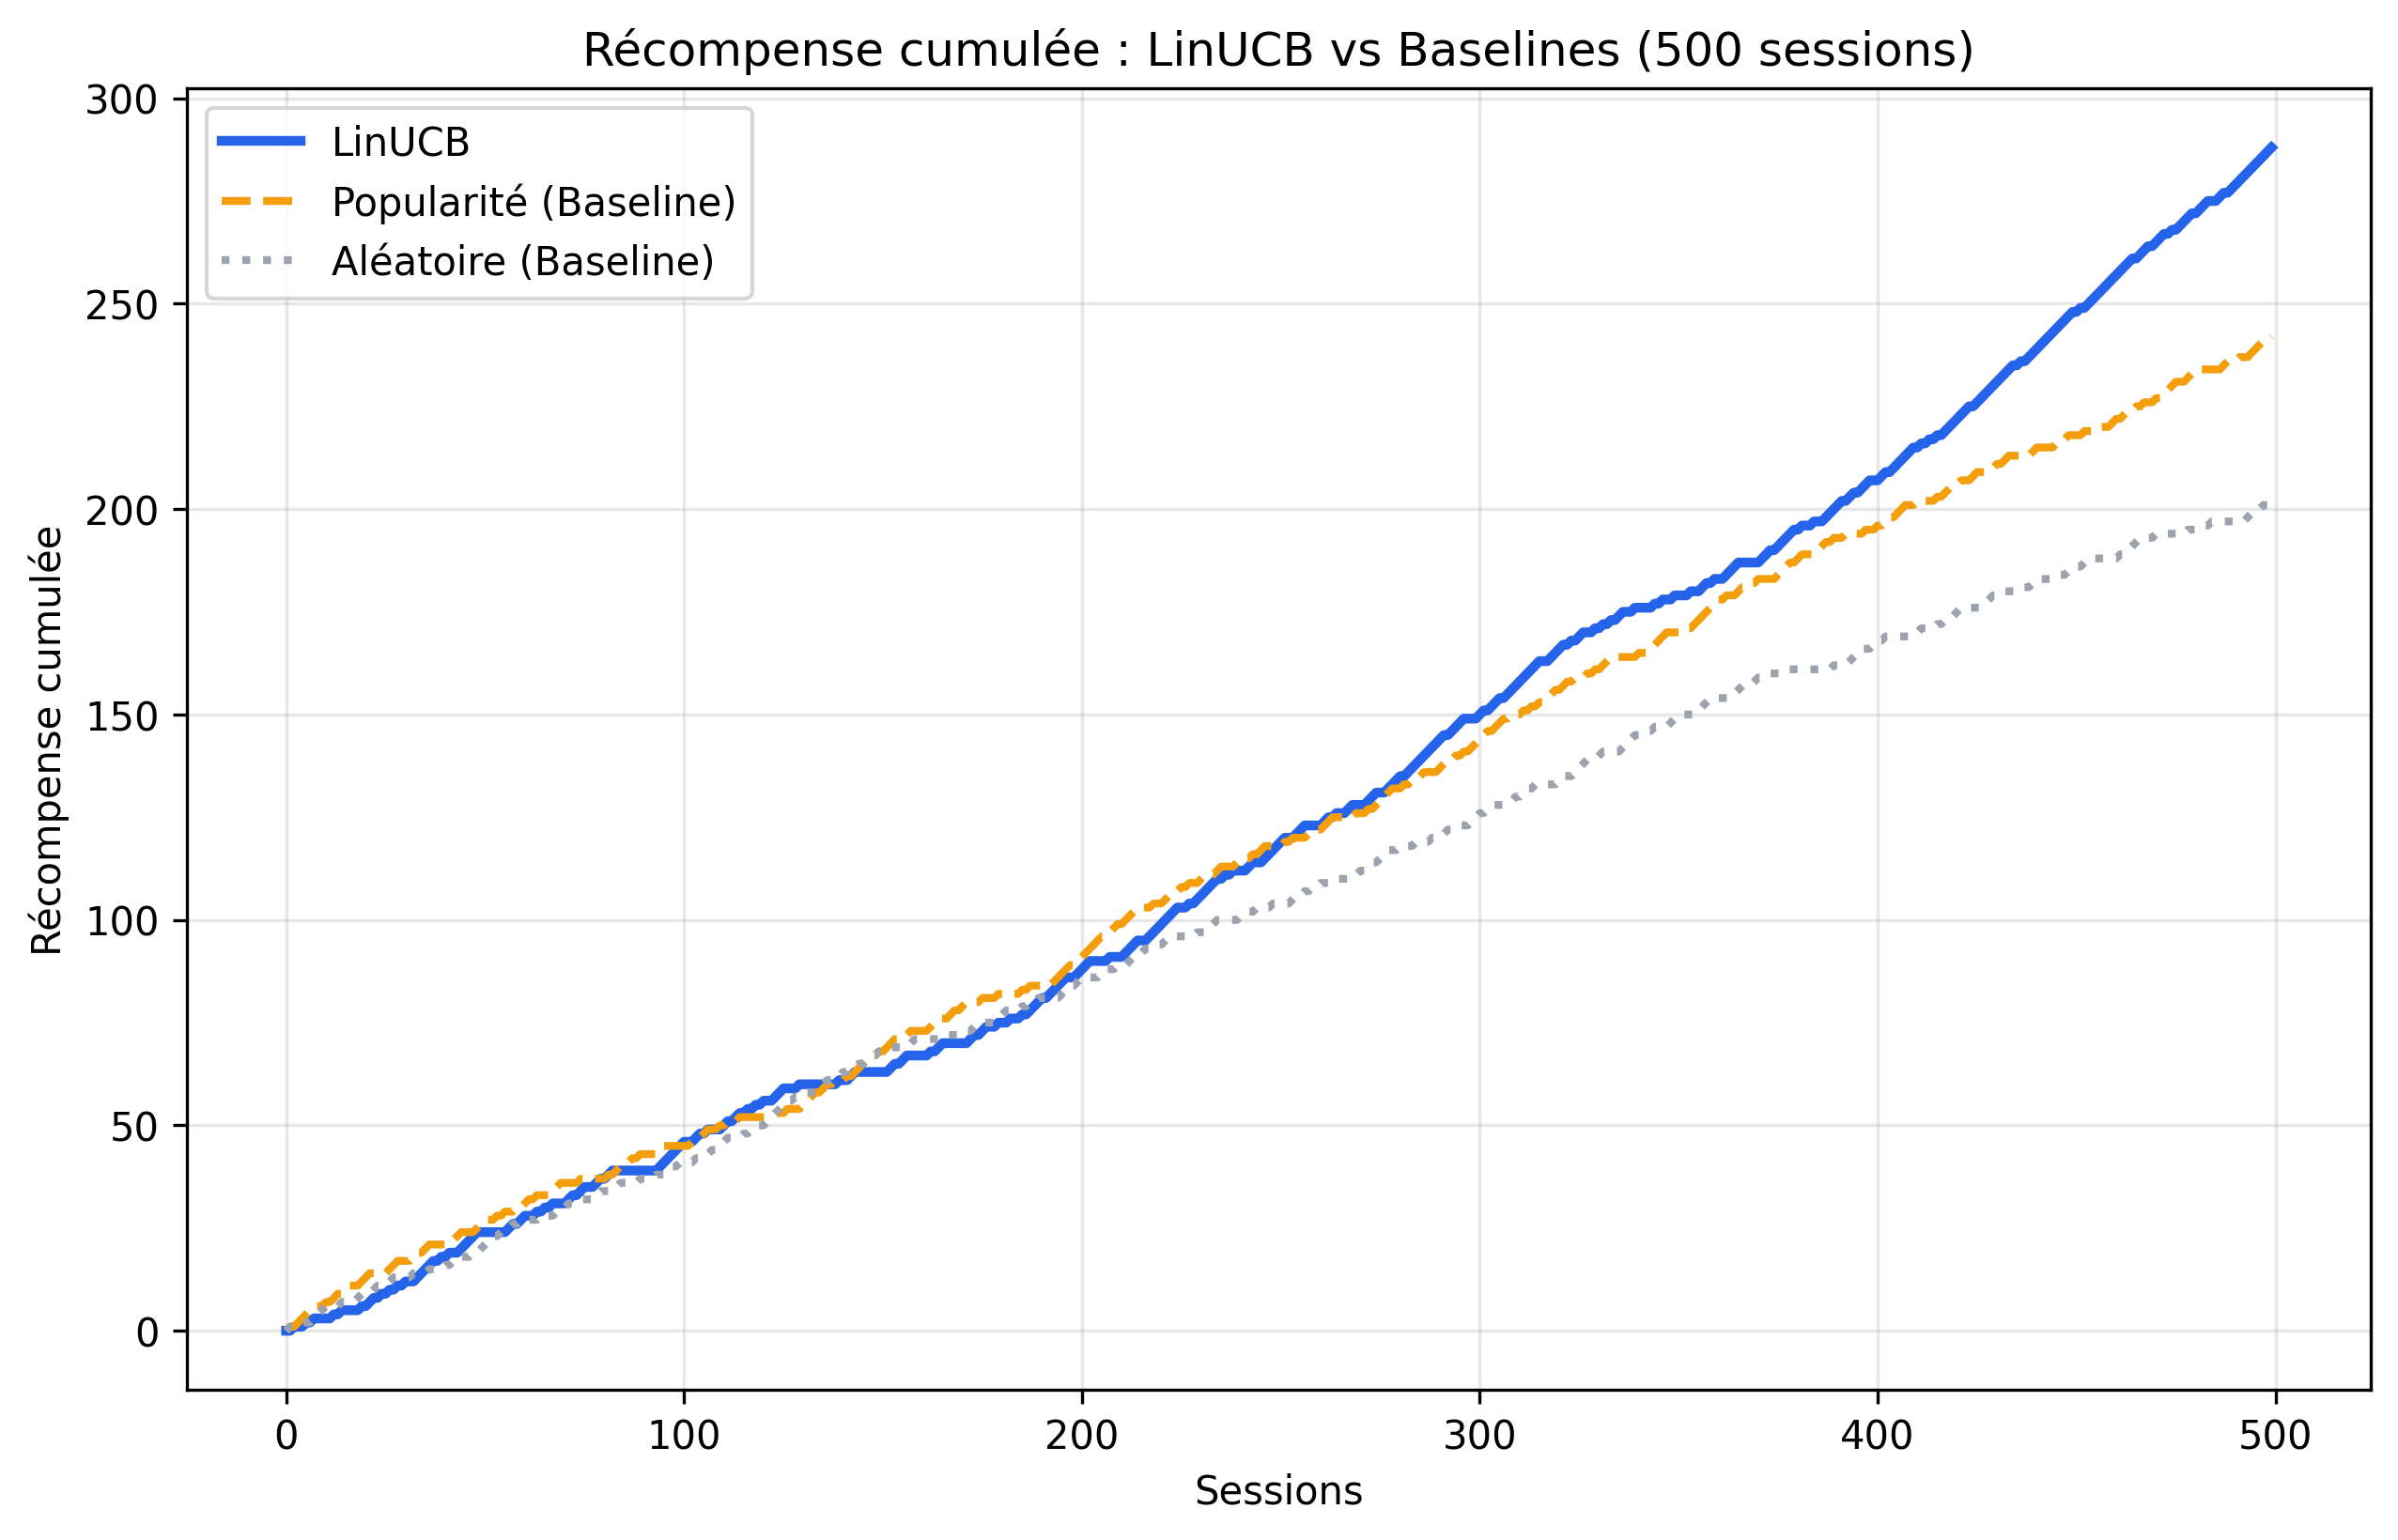
\includegraphics[width=0.85\textwidth]{diagrams/fig_06_cumulative_reward.png}
    \caption{Résultats de la simulation LinUCB (500 sessions)}
    \label{fig:linucb_simulation}
\end{figure}

\subsection{Recommandations affichées}

\begin{figure}[H]
    \centering
    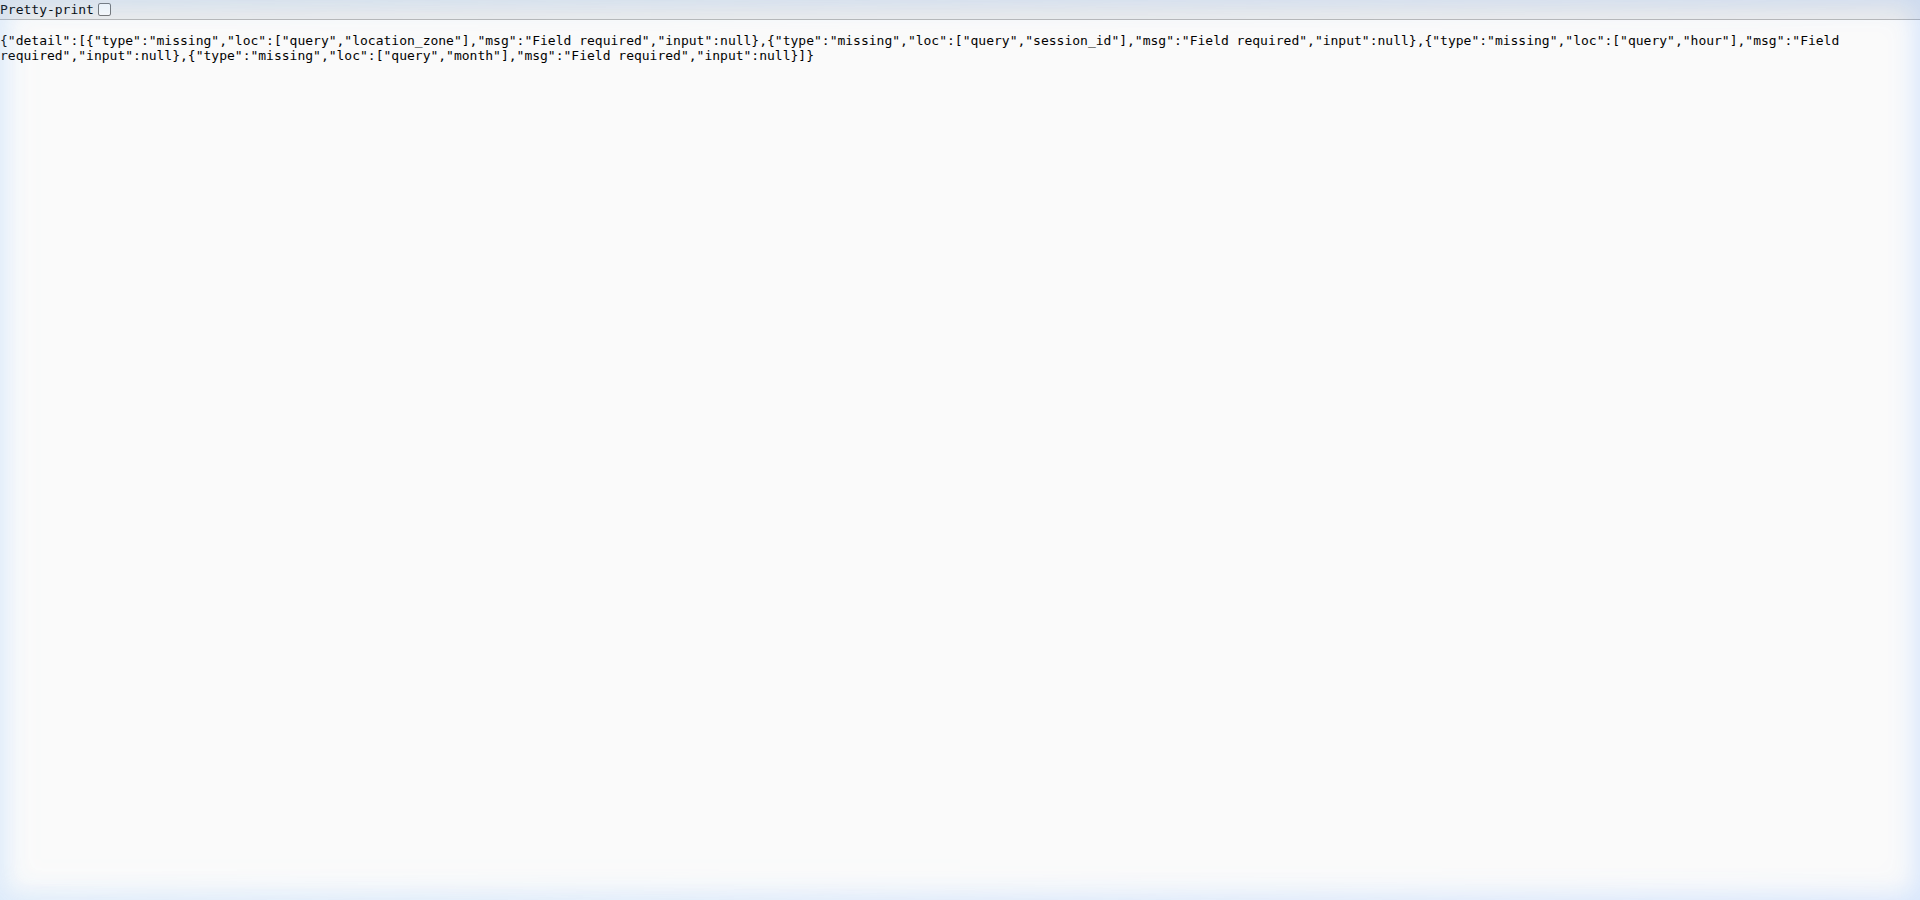
\includegraphics[width=\textwidth]{diagrams/screen_A4_recommendations_response.png}
    \caption{Recommandations personnalisées affichées sur la plateforme}
    \label{fig:screen_reco}
\end{figure}

\subsection{Supervision du système}

\begin{figure}[H]
    \centering
    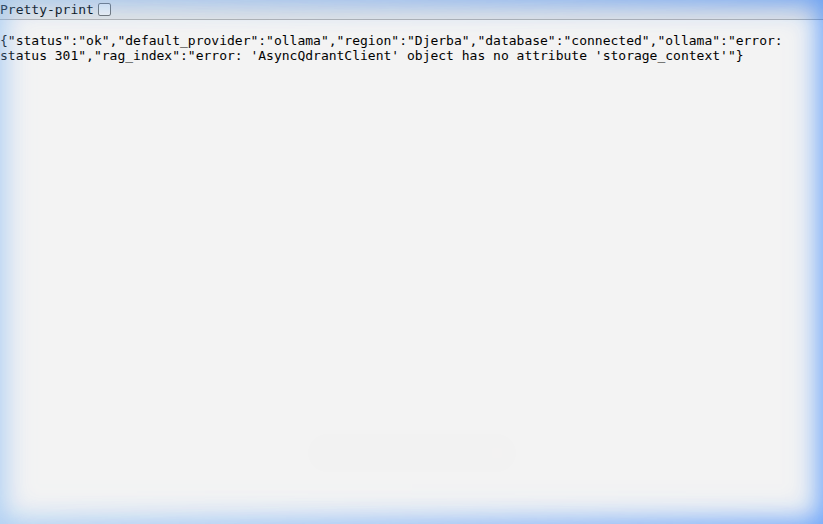
\includegraphics[width=\textwidth]{diagrams/screen_06_health_endpoint.png}
    \caption{Endpoint de santé du système avec statut des composants}
    \label{fig:screen_health_sprint4}
\end{figure}


% ────────────────────────────────────────────────────────────────
\section{Sprint Review}
% ────────────────────────────────────────────────────────────────

Lors de la Sprint Review finale, Guidni a été mis à l'essai dans un scénario continu simulant
une visite prolongée~: le raisonneur conversationnel combiné à l'affichage instantané des
recommandations LinUCB. L'ingestion de cent événements comportementaux via Postman a abouti
à une rotation des recommandations en faveur de séjours maritimes. La contrainte de latence
sous les 100~ms a été démontrée conforme, les chronomètres validant des inférences oscillant
entre 5 et 10~ms en condition locale.

L'encadrant a reconnu la satisfaction intégrale des prérequis fonctionnels et qualitatifs
du PFE. La Sprint Retrospective globale a consolidé un retour d'expérience édifiant sur
l'importance de l'organisation Scrum pour les systèmes d'IA évolutifs.


% ────────────────────────────────────────────────────────────────
\section*{Conclusion}
\addcontentsline{toc}{section}{Conclusion}

Le Sprint~4 a finalisé le développement du système Guidni par l'implémentation du moteur
de recommandation LinUCB avec son pipeline en 10~étapes, le tracker JavaScript, les jobs
nocturnes et les campagnes de tests et d'évaluation. Les simulations ont confirmé la
convergence prédictive du modèle et la satisfaction des contraintes de latence. Ce Sprint
conclut le cycle de développement itératif Scrum du projet Guidni. Le chapitre suivant
présentera la conclusion générale et les perspectives d'évolution future.


\chapter*{Conclusion Générale et Perspectives}
\addcontentsline{toc}{chapter}{Conclusion Générale et Perspectives}
% ============================================================================
% CHAPITRE 7 — CONCLUSION GÉNÉRALE ET PERSPECTIVES
% ============================================================================

\section*{Bilan du projet}
\addcontentsline{toc}{section}{Bilan du projet}

Le présent rapport de Projet de Fin d'Études rend compte de la conception, l'implémentation
et l'évaluation de \textbf{Guidni}, une plateforme de planification de voyage intelligente
dédiée à l'île de Djerba. En suivant rigoureusement la méthodologie Scrum sur quatre Sprints
(octobre 2024 -- février 2025), j'ai pu construire un système articulé autour de deux
sous-systèmes complémentaires.

Le premier sous-système, l'\textbf{Agent Planificateur conversationnel}, repose sur une
machine à états LangGraph à quatre nœuds (THINK, EXECUTE\_TOOL, VALIDATE, RESPOND) disposant
de dix-huit outils appelables par le LLM. Un pipeline RAG multilingue utilisant les embeddings
BAAI/bge-m3 (français, anglais, arabe) et un cross-encoder de réordonnancement garantissent
des réponses ancrées dans les données réelles du catalogue touristique de Djerba. L'abstraction
multi-fournisseurs LLM permet de basculer entre Ollama, Groq, Gemini et Lightning AI selon
les besoins. Le système de mémoire conversationnelle avec résumé automatique à 15~messages
assure la cohérence des conversations longues.

Le second sous-système, le \textbf{Moteur de Recommandation Hybride LinUCB}, exploite un
bandit contextuel avec un vecteur de caractéristiques de dimension~306 construit par produit
de Kronecker ($\phi = x_{\text{user}}(9) \otimes x_{\text{tags}}(34)$). Un pipeline de
classement post-traitement en dix étapes garantit la diversité, l'exploration et l'équité
des recommandations. Le cache matriciel en RAM avec verrou threading assure une latence de
scoring inférieure à 100~ms. Le tracker JavaScript vanilla collecte huit signaux
comportementaux en temps réel, alimentant l'apprentissage en ligne du modèle.

L'organisation Scrum s'est avérée déterminante pour tempérer les incertitudes inhérentes à
un projet d'intelligence artificielle. Les Sprint Reviews régulières ont permis de valider
chaque composant incrémentalement, et la Definition of Done a garanti un critère de qualité
objectif à chaque itération.


\section*{Perspectives et travaux futurs}
\addcontentsline{toc}{section}{Perspectives et travaux futurs}

Malgré les contributions apportées, plusieurs perspectives d'évolution se dégagent~:

\begin{enumerate}
    \item \textbf{Affinage d'un LLM local sur les données du tourisme tunisien.}
    L'historique de conversations stocké dans \texttt{PlannerMessage} constitue un corpus
    d'entraînement naturel. Un fine-tuning supervisé produirait un modèle domaine-spécifique
    comprenant la géographie locale et les niveaux de prix réalistes de Djerba.

    \item \textbf{Remplacement de LinUCB linéaire par un bandit neuronal.}
    Le modèle linéaire $r = \theta^\top \phi$ ne capture pas les interactions non linéaires
    complexes. Des architectures comme Neural UCB modéliseraient ces effets par un réseau de
    neurones tout en conservant la propriété UCB.

    \item \textbf{Infrastructure d'expérimentation A/B.}
    L'architecture actuelle ne permet pas de mesurer l'impact causal des changements
    algorithmiques. Un framework A/B permettrait de valider empiriquement les hypothèses
    d'amélioration avant déploiement.

    \item \textbf{Extension multi-régions.}
    Le champ \texttt{locationZone} est conçu pour supporter plusieurs zones géographiques.
    L'extension à Hammamet, Sousse et Tunis ne nécessite que l'ajout de données et
    l'initialisation des bras correspondants.

    \item \textbf{Interface vocale et multimodale.}
    L'intégration de la reconnaissance vocale arabe permettrait aux utilisateurs tunisiens
    de planifier leur voyage sans saisie clavier. Le pipeline RAG pourrait accepter des
    photos comme requêtes visuelles via des embeddings multimodaux.
\end{enumerate}


\section*{Mot de la fin}
\addcontentsline{toc}{section}{Mot de la fin}

Ce projet démontre que la combinaison de l'IA conversationnelle (agents LangGraph) et de
l'apprentissage en ligne (bandits contextuels) ouvre une nouvelle génération de plateformes
touristiques intelligentes~: simultanément personnalisées, adaptatives et ancrées dans des
données réelles. Le système Guidni est une preuve de concept opérationnelle démontrant que
cette combinaison est non seulement techniquement réalisable, mais pratiquement déployable
sur une infrastructure modeste~: un serveur unique avec Ollama local, une base de données
PostgreSQL standard et un tracker JavaScript sans aucune dépendance externe.


% ====================================================================
% BACK MATTER
% ====================================================================
\printbibliography

% ====================================================================
% APPENDICES
% ====================================================================
\appendix
\renewcommand{\chaptername}{Annexe}
\chapter{Annexes}
\addcontentsline{toc}{chapter}{Annexes}
% ============================================================================
% ANNEXES — sections/07_appendices.tex
% ============================================================================

% ─────────────────────────────────────────────────────────────────────────────
\section{Vocabulaire des tags (TAG\_VOCAB complet)}
\label{ann:tagvocab}
% ─────────────────────────────────────────────────────────────────────────────

Le vocabulaire de tags \texttt{TAG\_VOCAB} est une liste fixe de \textbf{40~tags} en ordre
alphabétique strict, définie dans \texttt{app/reco/context.py}. Il sert à structurer les thématiques des annonces pour la recherche sémantique RAG et l'indexation IA.
Dans l'ancienne implémentation LinUCB, la position de chaque tag était hautement critique car elle déterminait
son index dans le vecteur binaire $x_{tags}$ et son entrée dans les dimensions de la matrice d'apprentissage ($360 \times 360$) via un produit de Kronecker.
Avec la migration vers le système de recommandation \textbf{Hybrid Thompson Sampling}, cette dépendance complexe a été entièrement éliminée. Le moteur de recommandation actuel s'affranchit de cette contrainte dimensionnelle rigide en modélisant directement les bras par double segmentation contextuelle (globale via la destination et personnalisée via l'identifiant de l'utilisateur) sans nécessiter de produit de Kronecker ni de matrices multidimensionnelles globales, rendant le système extrêmement plus léger, performant en temps de calcul, et insensible aux évolutions futures du vocabulaire de tags.

\begin{center}
\captionof{table}{Vocabulaire complet des 40~tags (TAG\_VOCAB)}
\label{tab:tagvocab}
\footnotesize
\begin{longtable}{r p{3.2cm} p{2.5cm} p{6.5cm}}
    \toprule
    \textbf{Idx} & \textbf{Tag} & \textbf{Catégorie} & \textbf{Description} \\
    \midrule
    \endhead
    0  & \texttt{activity\_indoor}  & Activité    & Activité en intérieur (musée, atelier, salle de spectacle) \\
    1  & \texttt{activity\_outdoor} & Activité    & Activité en plein air (excursion, sport nautique, randonnée) \\
    2  & \texttt{adventure}         & Activité    & Activités à sensations (quad, jet-ski, escalade, kitesurf) \\
    3  & \texttt{air\_conditioning} & Commodité   & Hébergement ou espace climatisé \\
    4  & \texttt{airport\_transfer} & Transport   & Service de navette ou transfert aéroport inclus \\
    5  & \texttt{all\_seasons}      & Saison      & Disponible et pertinent toute l'année \\
    6  & \texttt{bar}               & Restauration & Bar ou lounge avec service de boissons \\
    7  & \texttt{beach\_access}     & Activité    & Accès direct ou à proximité immédiate d'une plage \\
    8  & \texttt{best\_evening}     & Moment      & Particulièrement adapté en soirée (coucher de soleil, dîner) \\
    9  & \texttt{best\_morning}     & Moment      & Mieux apprécié le matin (yoga, marché, plongée matinale) \\
    10 & \texttt{best\_summer}      & Saison      & Optimal en été (juin–septembre) \\
    11 & \texttt{best\_winter}      & Saison      & Recommandé en saison fraîche (novembre–mars) \\
    12 & \texttt{budget}            & Tarification & Prix accessible, option économique \\
    13 & \texttt{business}          & Ambiance    & Adapté aux voyageurs d'affaires \\
    14 & \texttt{casual\_dining}    & Restauration & Restaurant décontracté, cuisine informelle \\
    15 & \texttt{city}              & Localisation & Situé en zone urbaine (Houmt Souk, centre-ville) \\
    16 & \texttt{cultural}          & Activité    & Expérience culturelle, patrimoine, artisanat, histoire \\
    17 & \texttt{family}            & Ambiance    & Adapté aux familles avec enfants \\
    18 & \texttt{fine\_dining}      & Restauration & Restaurant gastronomique, service haut de gamme \\
    19 & \texttt{garden}            & Commodité   & Espace vert, jardin ou terrasse jardinée \\
    20 & \texttt{gym}               & Commodité   & Salle de sport ou espace fitness disponible \\
    21 & \texttt{hammam}            & Bien-être   & Hammam traditionnel ou bain maure \\
    22 & \texttt{hostel}            & Hébergement & Auberge de jeunesse, hébergement partagé \\
    23 & \texttt{hotel}             & Hébergement & Hôtel classique (1 à 5 étoiles) \\
    24 & \texttt{luxury}            & Tarification & Offre premium ou haut de gamme \\
    25 & \texttt{mountain\_view}    & Vue         & Vue sur les collines ou reliefs environnants \\
    26 & \texttt{nature}            & Localisation & Environnement naturel, loin de l'agitation urbaine \\
    27 & \texttt{parking}           & Commodité   & Parking privé ou sur place disponible \\
    28 & \texttt{pool}              & Commodité   & Piscine privée ou commune accessible \\
    29 & \texttt{private\_transfer} & Transport   & Transfert privatif sur demande \\
    30 & \texttt{riad}              & Hébergement & Maison traditionnelle à cour intérieure \\
    31 & \texttt{romantic}          & Ambiance    & Cadre romantique, idéal pour couples \\
    32 & \texttt{room\_service}     & Commodité   & Service en chambre disponible \\
    33 & \texttt{sea\_view}         & Vue         & Vue directe ou panoramique sur la mer \\
    34 & \texttt{solo}              & Ambiance    & Adapté aux voyageurs individuels \\
    35 & \texttt{spa}               & Bien-être   & Centre spa, soins, massages, thalasso \\
    36 & \texttt{street\_food}      & Restauration & Cuisine de rue, stands, marchés alimentaires \\
    37 & \texttt{terrace}           & Commodité   & Terrasse extérieure ou rooftop \\
    38 & \texttt{villa}             & Hébergement & Villa privée avec piscine ou jardin \\
    39 & \texttt{wifi}              & Commodité   & Connexion Wi-Fi disponible \\
    \bottomrule
\end{longtable}
\end{center}


% ─────────────────────────────────────────────────────────────────────────────
\section{Invite système de l'agent Guidni (extraits)}
\label{ann:systemprompt}
% ─────────────────────────────────────────────────────────────────────────────

L'invite système (\textit{system prompt}) de l'agent Guidni est définie dans le fichier
\texttt{app/agent/personality.py} sous la constante \texttt{SYSTEM\_PROMPT}. Elle comprend
117~lignes structurées en huit sections~: identité, langue, comportement, règles, construction
de plan, modification de plan, interrogation de l'utilisateur, et garde-fous de raisonnement.
Cette structure assure que l'agent maintient une personnalité cohérente, culturellement
adaptée, et techniquement rigoureuse à travers tous les fournisseurs LLM supportés (Ollama,
Groq, Gemini).

Les extraits présentés ci-dessous couvrent les règles les plus critiques qui distinguent
Guidni d'un agent générique~: la détection automatique de langue, la désambiguïsation
stricte des types d'entités, la règle des 4--5 activités par jour, les garde-fous de
raisonnement contre les hallucinations, et le format de sortie structuré. Ces règles sont
le résultat d'itérations d'ingénierie du prompt (\textit{prompt engineering}) visant à
réduire les erreurs structurelles détectées par le nœud VALIDATE.

\textbf{Extrait 1 — Identité et détection de langue automatique~:}

\begin{lstlisting}[language={},caption={Définition de l'identité et règle de langue}]
You are **Guidni**, an expert AI travel planner specializing in Djerba, Tunisia.

## Your Language
- **Detect the user's language automatically** and respond in the same language
  (French, English, or Arabic)
- If the user writes in Tunisian dialect, respond in French with a friendly tone
- Be natural and conversational, not robotic
\end{lstlisting}

\textbf{Extrait 2 — Règle de désambiguïsation des entités~:}

\begin{lstlisting}[language={},caption={Règles strictes de classification des types d'entités}]
CRITICAL -- Entity Type Rules:
- **activity** = things to DO during the day (tours, sports, sightseeing).
  Put these in daytime plan slots.
- **stay** = ACCOMMODATION (hotels, villas, guesthouses). Suggest as overnight
  stay ONLY. NEVER list a stay as a daytime activity.
- **restaurant** = places to EAT. Use for lunch/dinner meal slots only.
- **attraction** = free sightseeing spots. Use in daytime plan slots.
A stay with "Beach" or "Spa" in its name is still a HOTEL, not a beach activity.
Do NOT confuse them.
\end{lstlisting}

\textbf{Extrait 3 — Règle des activités par jour et obligation des repas~:}

\begin{lstlisting}[language={},caption={Règles de densité journalière du plan}]
4. **Maximum 4-5 activities per day** -- people need rest, travel time,
   and spontaneity
5. **Always include meals** -- suggest restaurants for lunch and dinner
6. **Include rest/free time** -- especially for relaxed travel styles
\end{lstlisting}

\textbf{Extrait 4 — Garde-fou anti-hallucination et seuil de confiance RAG~:}

\begin{lstlisting}[language={},caption={Garde-fous de raisonnement contre les hallucinations}]
### 2. CONTEXT WINDOW HYGIENE
- **NEVER hallucinate**: Only suggest places, prices, and locations explicitly
  returned by tools (SQL or RAG).
- If a place/activity is not in tool results, say it's unavailable --
  do NOT fabricate it.
- Only use IDs and metadata provided by tools. Never invent opening hours
  or addresses.

### 3. THE REASONING LOOP (THINK -> ACT -> OBSERVE)
- Aim to complete the plan in **under 6 iterations**.
- Use "Confidence Threshold": If RAG results have a high score (>0.7) and
  match the user's theme, trust them and move to planning.
\end{lstlisting}

\textbf{Extrait 5 — Format de sortie structuré~:}

\begin{lstlisting}[language={},caption={Contrainte de format de sortie du plan généré}]
### 6. FINAL OUTPUT FORMAT
- Produce a structured plan strictly matching the GeneratedPlan schema.
- If any required field is missing from tool data, mark it as
  "Review Required" instead of guessing.
- Every activity and restaurant in the plan MUST have a real entity ID
  from tool results.
\end{lstlisting}


% ─────────────────────────────────────────────────────────────────────────────
\section{Extraits du schéma de base de données}
\label{ann:schema}
% ─────────────────────────────────────────────────────────────────────────────

Le système Guidni utilise une architecture de base de données partagée où deux sous-systèmes
coexistent dans la même instance PostgreSQL~: le sous-système planificateur (géré via
SQLAlchemy par l'agent Python) et le sous-système de recommandation (géré via Prisma par le
frontend Next.js). La partition est stricte~: les tables liées à la planification (\texttt{PlannerConversation},
\texttt{PlannerMessage}, \texttt{GeneratedPlan}, \texttt{ActivityIntelligence}) sont en
écriture exclusive par l'agent Python, tandis que les tables du frontend (\texttt{Activity},
\texttt{Stay}, \texttt{Restaurant}, etc.) sont montées en lecture seule pour l'agent via les modèles
SQLAlchemy correspondants. C'est d'ailleurs sur ces tables partagées que sont déployés les \textbf{triggers SQL}, 
écoutant les modifications effectuées par le frontend pour déclencher la réindexation asynchrone de l'agent.

Les tables du moteur de recommandation (\texttt{BanditArm}, \texttt{RecommendationEvent}) sont définies dans \texttt{prisma/schema.prisma} mais exploitées principalement via des requêtes SQL directes dans \texttt{app/reco/db.py} en utilisant un pool synchrone threadé. Cette approche évite l'utilisation d'anciennes structures complexes et lourdes comme les profils d'affinités de tags matriciels ou le stockage de matrices d'apprentissage global, ce qui simplifie radicalement la persistance de l'apprentissage en ligne de la recommandation.

\textbf{Modèles planificateur (SQLAlchemy — tables propriétaires de l'agent)~:}

\begin{lstlisting}[language=Python, caption={Modèles SQLAlchemy du planificateur (app/db/models.py)}]
class PlannerConversation(Base):
    __tablename__ = "PlannerConversation"
    id             = Column(String, primary_key=True)
    userId         = Column(String, ForeignKey("User.id"), nullable=False)
    title          = Column(String, nullable=True)
    contextSummary = Column(JSON, nullable=True)   # LLM-generated summary
    isActive       = Column(Boolean, default=True)
    createdAt      = Column(DateTime, default=datetime.utcnow)
    updatedAt      = Column(DateTime, default=datetime.utcnow)

class PlannerMessage(Base):
    __tablename__ = "PlannerMessage"
    id             = Column(String, primary_key=True)
    conversationId = Column(String, ForeignKey("PlannerConversation.id"))
    role           = Column(String, nullable=False)  # "user"|"assistant"|"system"
    content        = Column(Text, nullable=False)
    messageType    = Column(String, default="text")  # "text"|"plan"|"question"
    meta_data      = Column("metadata", JSON, nullable=True)  # thinking_steps
    createdAt      = Column(DateTime, default=datetime.utcnow)

class GeneratedPlan(Base):
    __tablename__ = "GeneratedPlan"
    id             = Column(String, primary_key=True)
    conversationId = Column(String, ForeignKey("PlannerConversation.id"))
    userId         = Column(String, ForeignKey("User.id"), nullable=False)
    planData       = Column(JSON, nullable=False)   # Full FullPlan JSON
    version        = Column(Integer, default=1)
    isActive       = Column(Boolean, default=True)
    createdAt      = Column(DateTime, default=datetime.utcnow)
    updatedAt      = Column(DateTime, default=datetime.utcnow)

class ActivityIntelligence(Base):
    __tablename__ = "ActivityIntelligence"
    id             = Column(String, primary_key=True)
    activityId     = Column(String, ForeignKey("Activity.id"), unique=True)
    enrichmentData = Column(JSON, nullable=False)  # AI enrichment cache
    createdAt      = Column(DateTime, default=datetime.utcnow)
    updatedAt      = Column(DateTime, default=datetime.utcnow)
\end{lstlisting}

\textbf{Modèles de recommandation (Prisma — extraits de \texttt{prisma/schema.prisma})~:}

\begin{lstlisting}[language={},caption={Modèles Prisma du moteur Thompson Sampling (prisma/schema.prisma)}]
model RecommendationEvent {
  id          String   @id @default(cuid())
  eventType   String   // "impression" | "click" | "dwell_time" | "gallery_swipe" | "wishlist" | "reservation"
  listingId   String
  listingType String   // "ACTIVITY" | "STAY" | "RESTAURANT" | "RENTAL" | "TRANSFER"
  userId      String?  // null for anonymous
  sessionId   String   // browser sessionStorage ID
  segment     String   // context segment key
  reward      Float    // computed alpha delta
  price       Float?   // for reservation events
  metadata    Json?    // { position, page, dwellMs, swipeCount }
  createdAt   DateTime @default(now())

  @@index([listingId, listingType])
  @@index([segment])
  @@index([eventType])
  @@index([createdAt])
}

model BanditArm {
  id           String   @id @default(cuid())
  listingId    String
  listingType  String
  segment      String   // context segment key
  alpha        Float    @default(1.0)  // successes (prior=1)
  beta         Float    @default(1.0)  // failures (prior=1)
  impressions  Int      @default(0)
  clicks       Int      @default(0)
  wishlists    Int      @default(0)
  conversions  Int      @default(0)
  totalRevenue Float    @default(0.0)
  updatedAt    DateTime @updatedAt

  @@unique([listingId, listingType, segment])
  @@index([segment])
  @@index([listingType, segment])
}
\end{lstlisting}


% ─────────────────────────────────────────────────────────────────────────────
\section{Captures d'écran de l'application}
\label{ann:screenshots}
% ─────────────────────────────────────────────────────────────────────────────

Les captures d'écran suivantes illustrent les interfaces principales et les réponses API
du système Guidni dans son état opérationnel. Elles documentent visuellement les composants
décrits tout au long du rapport~: l'interface conversationnelle de l'agent, le format de
plan généré, les endpoints de diagnostic, et la réponse du moteur de recommandation avec
les scores détaillés. Ces captures constituent une référence pour la validation fonctionnelle
et le débogage en production.

\begin{figure}[H]
    \centering
    
\includegraphics[width=\textwidth]{diagrams/screen_A4_chat_interface.png}
    \caption{Interface de chat de l'agent planificateur Guidni}
    \label{fig:A1_chat}
\end{figure}

\begin{figure}[H]
    \centering
    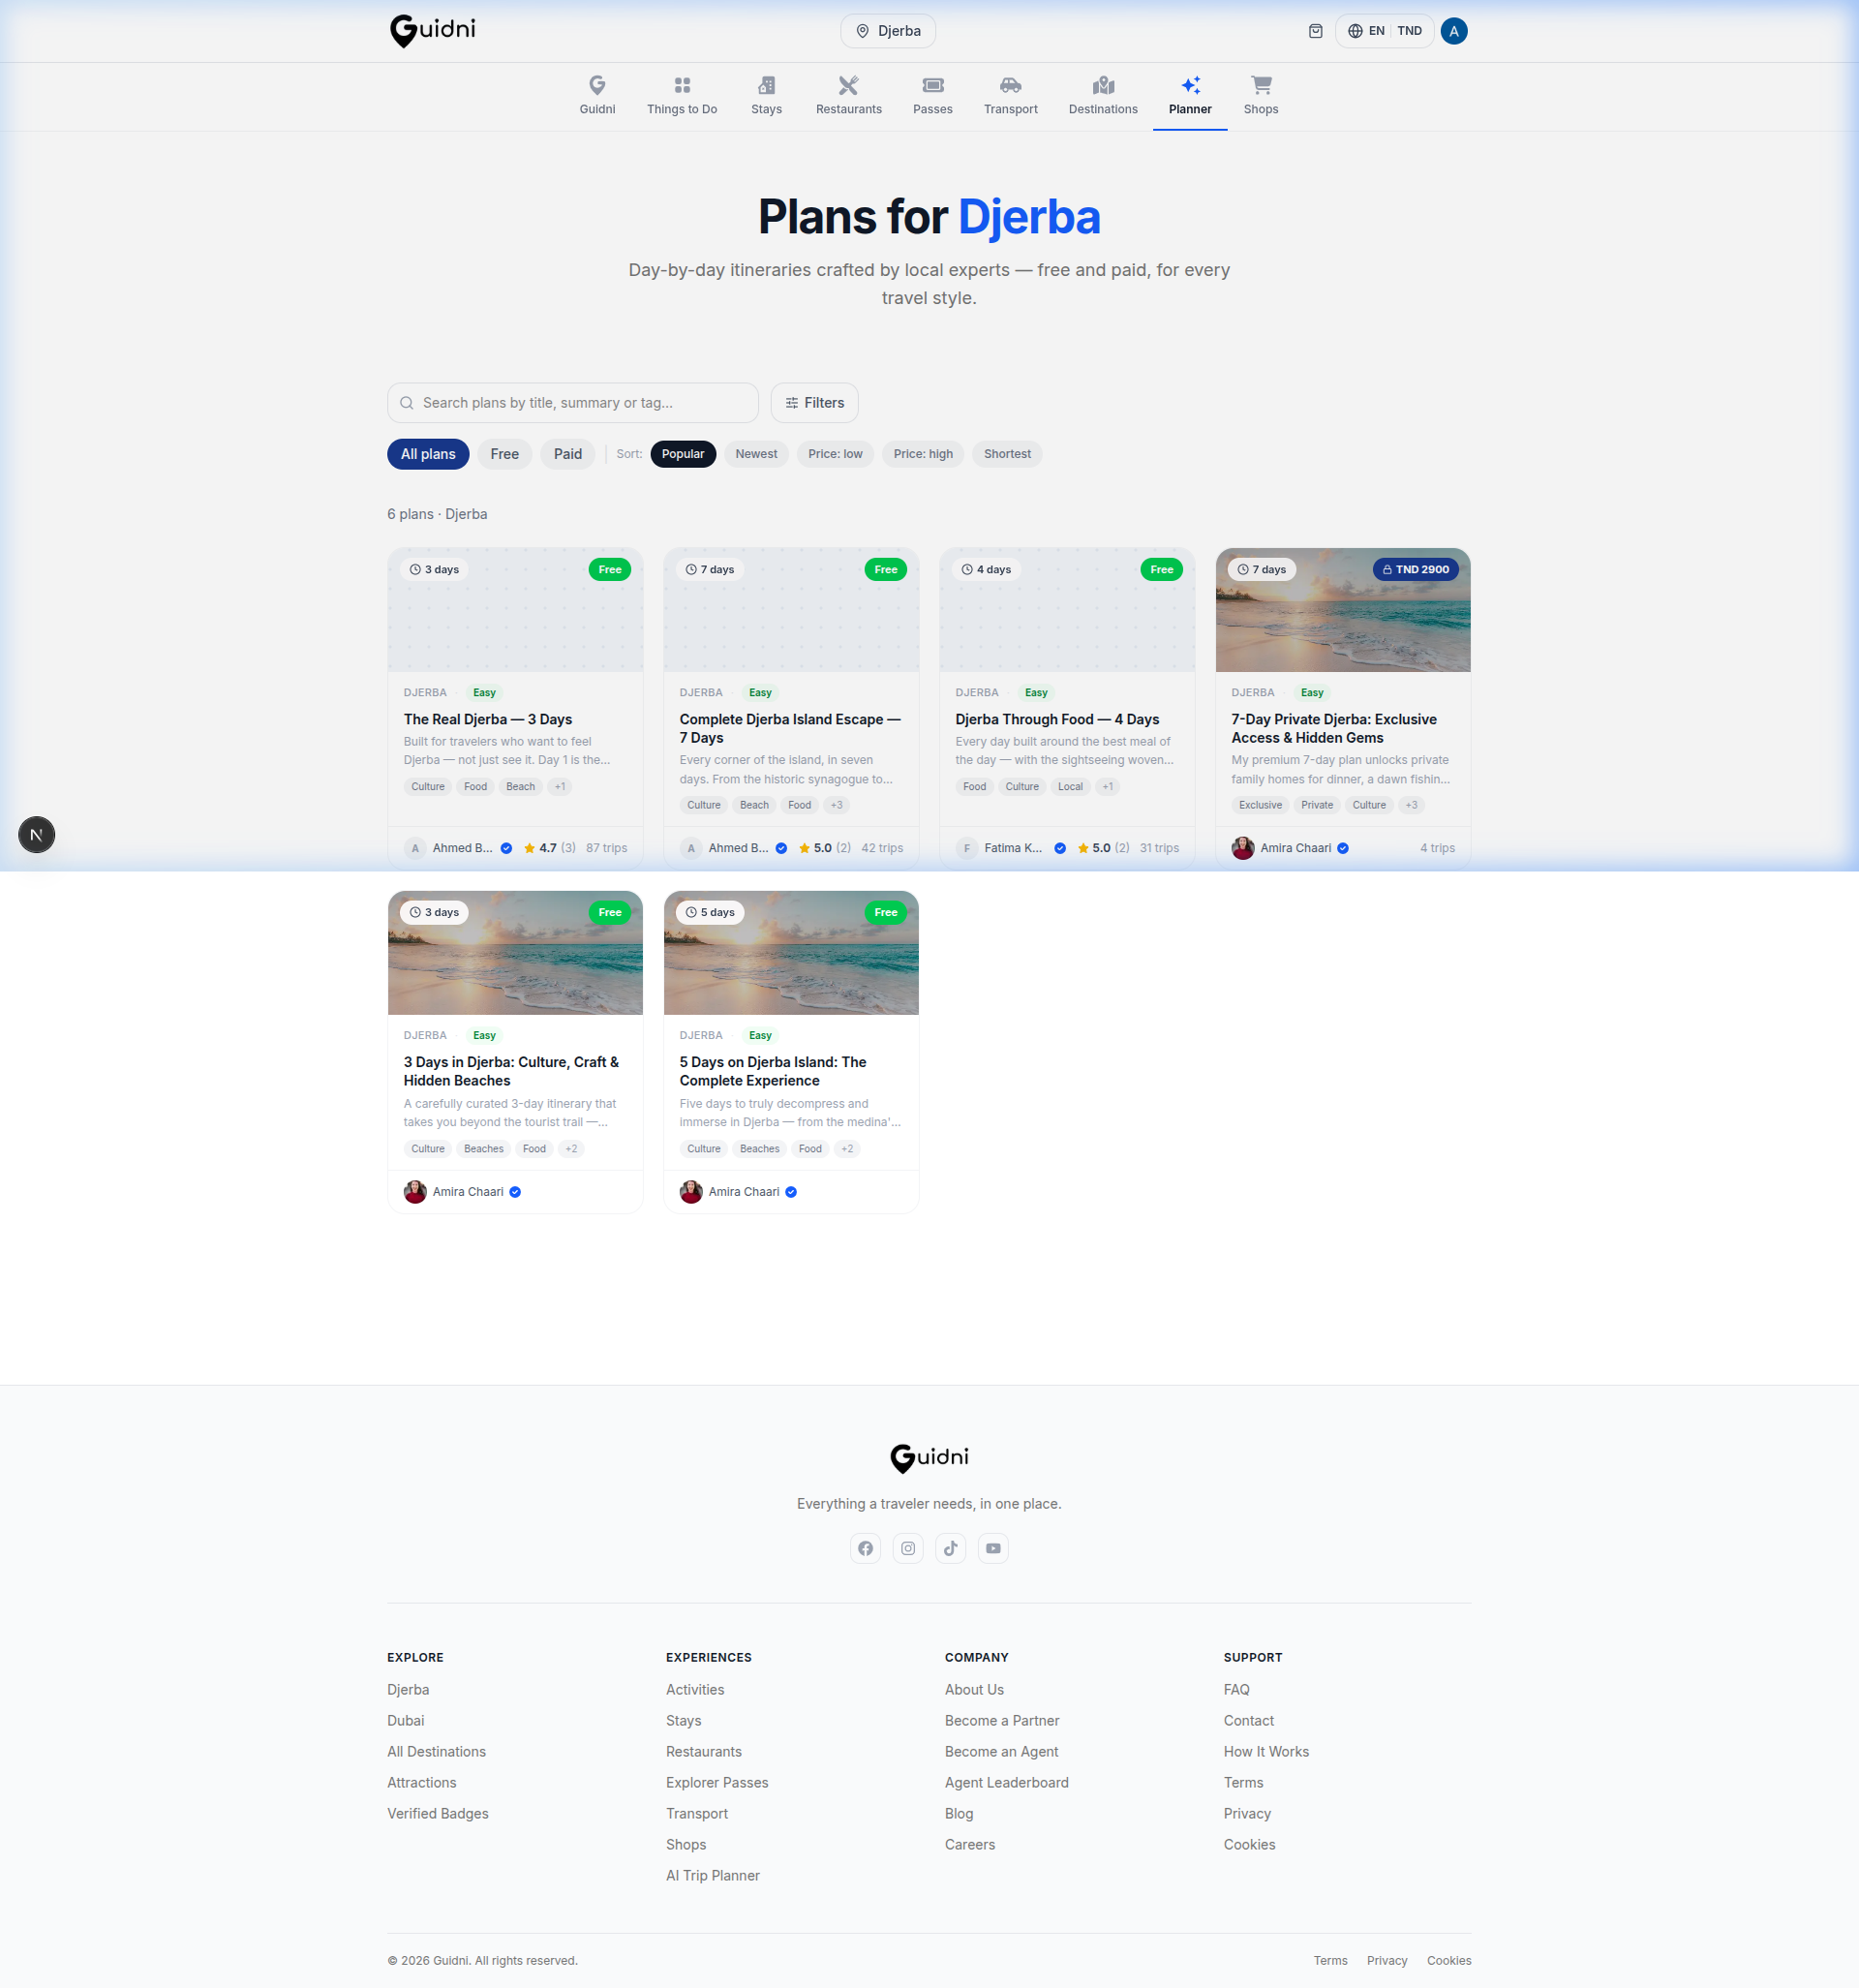
\includegraphics[width=\textwidth]{diagrams/screen_A4_plan_output_full.png}
    \caption{Exemple complet de plan de voyage généré (5 jours, famille)}
    \label{fig:A2_plan}
\end{figure}

\begin{figure}[H]
    \centering
    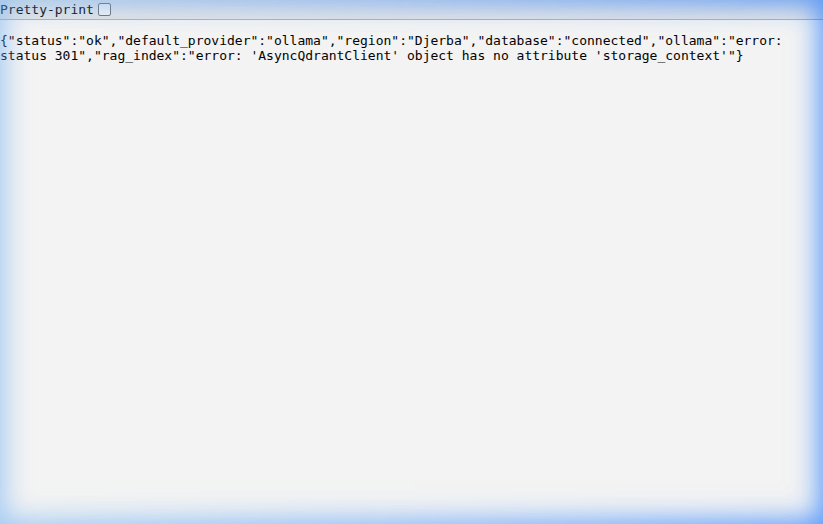
\includegraphics[width=\textwidth]{diagrams/screen_A4_health_check.png}
    \caption{Réponse complète de l'endpoint /health}
    \label{fig:A3_health}
\end{figure}

\begin{figure}[H]
    \centering
    
\includegraphics[width=\textwidth]{diagrams/screen_A4_admin_rebuild.png}
    \caption{Endpoint /admin/rebuild-index après reconstruction complète de l'index RAG}
    \label{fig:A4_rebuild}
\end{figure}

\begin{figure}[H]
    \centering
    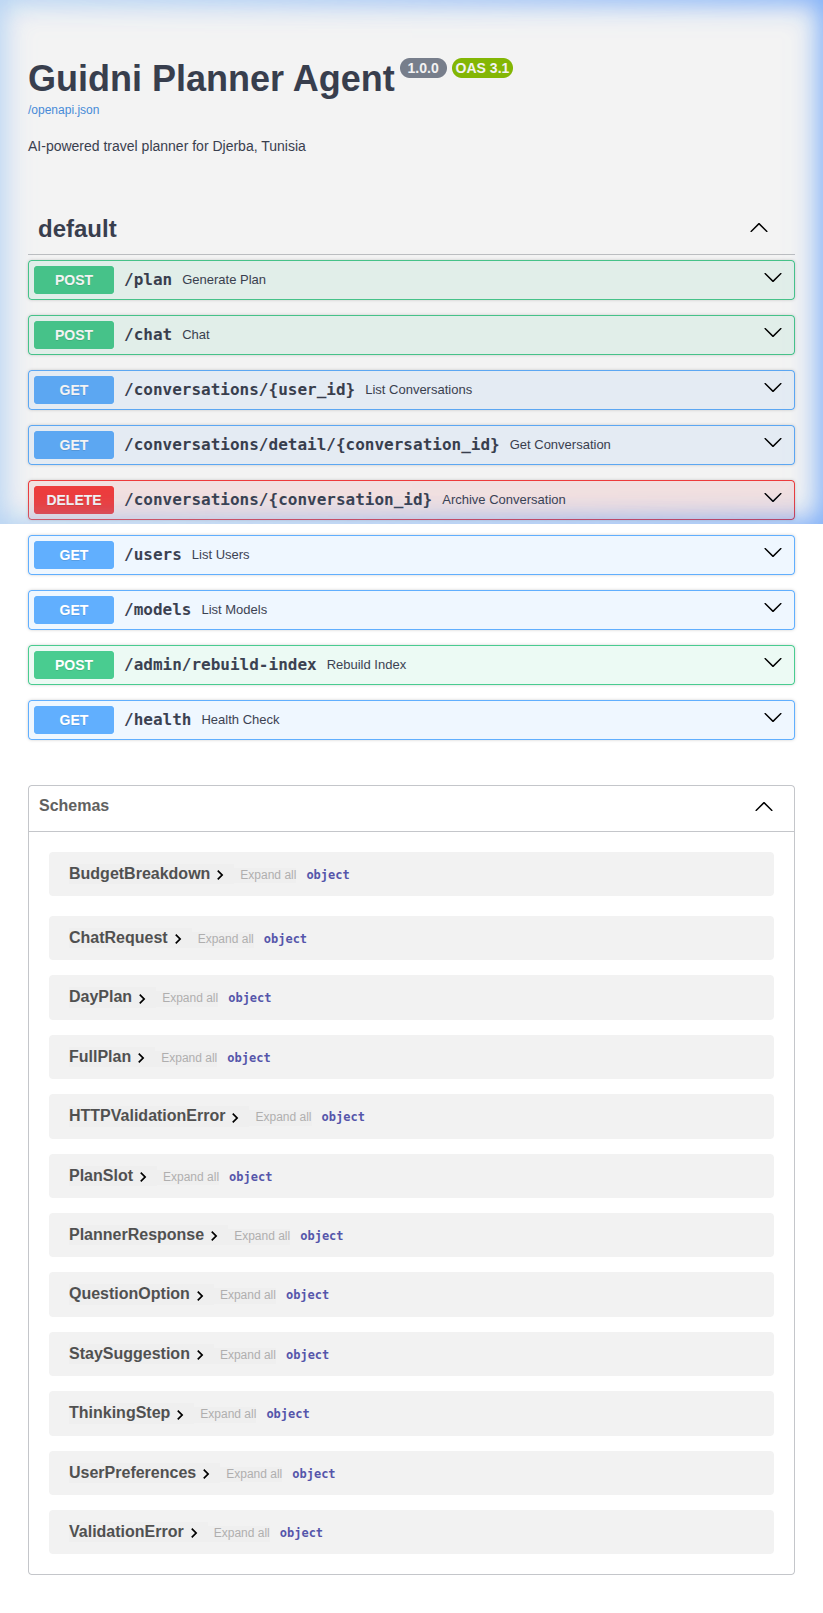
\includegraphics[width=\textwidth]{diagrams/screen_A4_api_docs.png}
    \caption{Documentation OpenAPI auto-générée par FastAPI (/docs)}
    \label{fig:A5_docs}
\end{figure}

\begin{figure}[H]
    \centering
    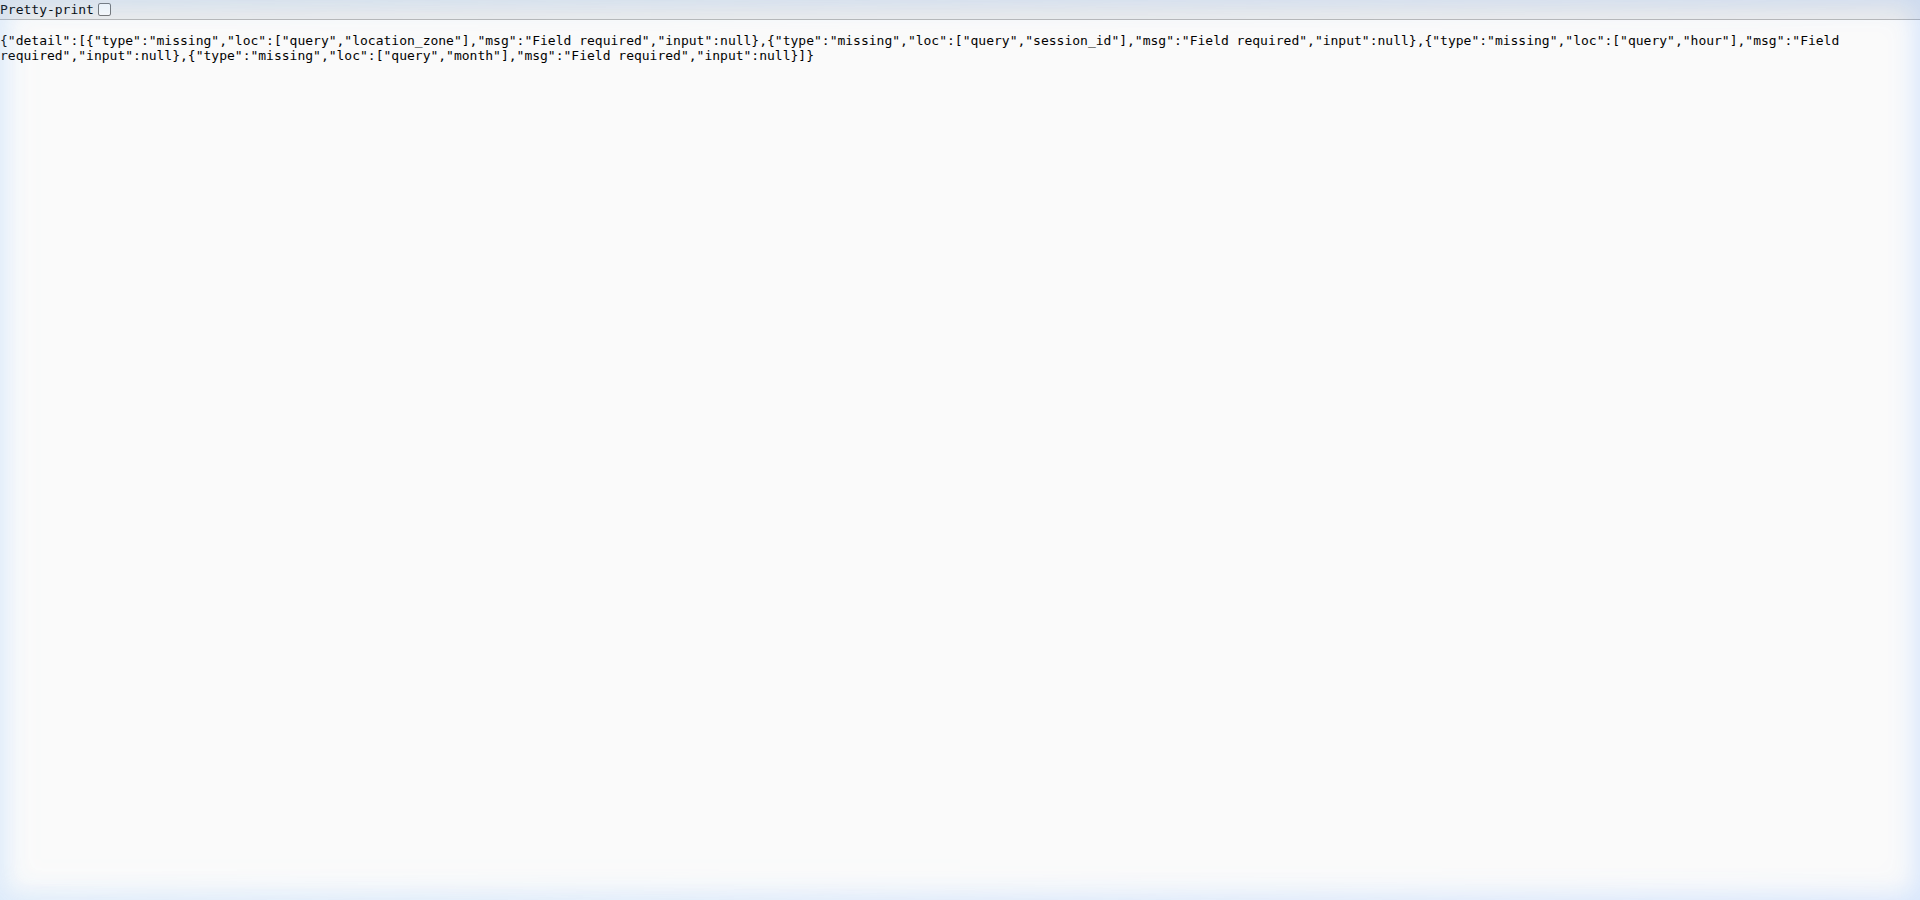
\includegraphics[width=\textwidth]{diagrams/screen_A4_recommendations_response.png}
    \caption{Exemple de réponse de l'API /api/recommend/feed avec paramètres $\alpha$ et $\beta$ exposés pour le diagnostic}
    \label{fig:A6_scores}
\end{figure}


\end{document}
